% Options for packages loaded elsewhere
\PassOptionsToPackage{unicode}{hyperref}
\PassOptionsToPackage{hyphens}{url}
%
\documentclass[
]{article}
\usepackage{amsmath,amssymb}
\usepackage{lmodern}
\usepackage{ifxetex,ifluatex}
\ifnum 0\ifxetex 1\fi\ifluatex 1\fi=0 % if pdftex
  \usepackage[T1]{fontenc}
  \usepackage[utf8]{inputenc}
  \usepackage{textcomp} % provide euro and other symbols
\else % if luatex or xetex
  \usepackage{unicode-math}
  \defaultfontfeatures{Scale=MatchLowercase}
  \defaultfontfeatures[\rmfamily]{Ligatures=TeX,Scale=1}
\fi
% Use upquote if available, for straight quotes in verbatim environments
\IfFileExists{upquote.sty}{\usepackage{upquote}}{}
\IfFileExists{microtype.sty}{% use microtype if available
  \usepackage[]{microtype}
  \UseMicrotypeSet[protrusion]{basicmath} % disable protrusion for tt fonts
}{}
\makeatletter
\@ifundefined{KOMAClassName}{% if non-KOMA class
  \IfFileExists{parskip.sty}{%
    \usepackage{parskip}
  }{% else
    \setlength{\parindent}{0pt}
    \setlength{\parskip}{6pt plus 2pt minus 1pt}}
}{% if KOMA class
  \KOMAoptions{parskip=half}}
\makeatother
\usepackage{xcolor}
\IfFileExists{xurl.sty}{\usepackage{xurl}}{} % add URL line breaks if available
\IfFileExists{bookmark.sty}{\usepackage{bookmark}}{\usepackage{hyperref}}
\hypersetup{
  pdftitle={Visualizing Probability Distributions with ggplot},
  pdfauthor={Ben Wallace},
  hidelinks,
  pdfcreator={LaTeX via pandoc}}
\urlstyle{same} % disable monospaced font for URLs
\usepackage[margin=1in]{geometry}
\usepackage{color}
\usepackage{fancyvrb}
\newcommand{\VerbBar}{|}
\newcommand{\VERB}{\Verb[commandchars=\\\{\}]}
\DefineVerbatimEnvironment{Highlighting}{Verbatim}{commandchars=\\\{\}}
% Add ',fontsize=\small' for more characters per line
\usepackage{framed}
\definecolor{shadecolor}{RGB}{248,248,248}
\newenvironment{Shaded}{\begin{snugshade}}{\end{snugshade}}
\newcommand{\AlertTok}[1]{\textcolor[rgb]{0.94,0.16,0.16}{#1}}
\newcommand{\AnnotationTok}[1]{\textcolor[rgb]{0.56,0.35,0.01}{\textbf{\textit{#1}}}}
\newcommand{\AttributeTok}[1]{\textcolor[rgb]{0.77,0.63,0.00}{#1}}
\newcommand{\BaseNTok}[1]{\textcolor[rgb]{0.00,0.00,0.81}{#1}}
\newcommand{\BuiltInTok}[1]{#1}
\newcommand{\CharTok}[1]{\textcolor[rgb]{0.31,0.60,0.02}{#1}}
\newcommand{\CommentTok}[1]{\textcolor[rgb]{0.56,0.35,0.01}{\textit{#1}}}
\newcommand{\CommentVarTok}[1]{\textcolor[rgb]{0.56,0.35,0.01}{\textbf{\textit{#1}}}}
\newcommand{\ConstantTok}[1]{\textcolor[rgb]{0.00,0.00,0.00}{#1}}
\newcommand{\ControlFlowTok}[1]{\textcolor[rgb]{0.13,0.29,0.53}{\textbf{#1}}}
\newcommand{\DataTypeTok}[1]{\textcolor[rgb]{0.13,0.29,0.53}{#1}}
\newcommand{\DecValTok}[1]{\textcolor[rgb]{0.00,0.00,0.81}{#1}}
\newcommand{\DocumentationTok}[1]{\textcolor[rgb]{0.56,0.35,0.01}{\textbf{\textit{#1}}}}
\newcommand{\ErrorTok}[1]{\textcolor[rgb]{0.64,0.00,0.00}{\textbf{#1}}}
\newcommand{\ExtensionTok}[1]{#1}
\newcommand{\FloatTok}[1]{\textcolor[rgb]{0.00,0.00,0.81}{#1}}
\newcommand{\FunctionTok}[1]{\textcolor[rgb]{0.00,0.00,0.00}{#1}}
\newcommand{\ImportTok}[1]{#1}
\newcommand{\InformationTok}[1]{\textcolor[rgb]{0.56,0.35,0.01}{\textbf{\textit{#1}}}}
\newcommand{\KeywordTok}[1]{\textcolor[rgb]{0.13,0.29,0.53}{\textbf{#1}}}
\newcommand{\NormalTok}[1]{#1}
\newcommand{\OperatorTok}[1]{\textcolor[rgb]{0.81,0.36,0.00}{\textbf{#1}}}
\newcommand{\OtherTok}[1]{\textcolor[rgb]{0.56,0.35,0.01}{#1}}
\newcommand{\PreprocessorTok}[1]{\textcolor[rgb]{0.56,0.35,0.01}{\textit{#1}}}
\newcommand{\RegionMarkerTok}[1]{#1}
\newcommand{\SpecialCharTok}[1]{\textcolor[rgb]{0.00,0.00,0.00}{#1}}
\newcommand{\SpecialStringTok}[1]{\textcolor[rgb]{0.31,0.60,0.02}{#1}}
\newcommand{\StringTok}[1]{\textcolor[rgb]{0.31,0.60,0.02}{#1}}
\newcommand{\VariableTok}[1]{\textcolor[rgb]{0.00,0.00,0.00}{#1}}
\newcommand{\VerbatimStringTok}[1]{\textcolor[rgb]{0.31,0.60,0.02}{#1}}
\newcommand{\WarningTok}[1]{\textcolor[rgb]{0.56,0.35,0.01}{\textbf{\textit{#1}}}}
\usepackage{longtable,booktabs,array}
\usepackage{calc} % for calculating minipage widths
% Correct order of tables after \paragraph or \subparagraph
\usepackage{etoolbox}
\makeatletter
\patchcmd\longtable{\par}{\if@noskipsec\mbox{}\fi\par}{}{}
\makeatother
% Allow footnotes in longtable head/foot
\IfFileExists{footnotehyper.sty}{\usepackage{footnotehyper}}{\usepackage{footnote}}
\makesavenoteenv{longtable}
\usepackage{graphicx}
\makeatletter
\def\maxwidth{\ifdim\Gin@nat@width>\linewidth\linewidth\else\Gin@nat@width\fi}
\def\maxheight{\ifdim\Gin@nat@height>\textheight\textheight\else\Gin@nat@height\fi}
\makeatother
% Scale images if necessary, so that they will not overflow the page
% margins by default, and it is still possible to overwrite the defaults
% using explicit options in \includegraphics[width, height, ...]{}
\setkeys{Gin}{width=\maxwidth,height=\maxheight,keepaspectratio}
% Set default figure placement to htbp
\makeatletter
\def\fps@figure{htbp}
\makeatother
\setlength{\emergencystretch}{3em} % prevent overfull lines
\providecommand{\tightlist}{%
  \setlength{\itemsep}{0pt}\setlength{\parskip}{0pt}}
\setcounter{secnumdepth}{5}
\usepackage{booktabs}
\usepackage{amsthm}
\makeatletter
\def\thm@space@setup{%
  \thm@preskip=8pt plus 2pt minus 4pt
  \thm@postskip=\thm@preskip
}
\makeatother

%% New Commands

\newcommand{\smspace}{\hspace{0.2}}}
\newcommand{\medspace}{\hspace{0.7}}}

\ifluatex
  \usepackage{selnolig}  % disable illegal ligatures
\fi
\usepackage[]{natbib}
\bibliographystyle{apalike}

\title{Visualizing Probability Distributions with ggplot}
\author{Ben Wallace}
\date{2021-08-11}

\begin{document}
\maketitle

{
\setcounter{tocdepth}{2}
\tableofcontents
}
\hypertarget{introduction}{%
\section{Introduction}\label{introduction}}

This is a guide to understanding and visualizing several important discrete and continuous distributions in the statistics world. We will use several R packages in the process.

\begin{itemize}
\item
  \texttt{stats} (installed by default in RStudio) to retrieve statistical distributions.
\item
  \texttt{tidyverse} to coerce data into \href{https://r4ds.had.co.nz/tibbles.html}{tidy} format and produce visualizations with \texttt{ggplot}.
\end{itemize}

\begin{Shaded}
\begin{Highlighting}[]
\FunctionTok{install.packages}\NormalTok{(}\StringTok{"tidyverse"}\NormalTok{) }\CommentTok{\# Includes both tibble and ggplot2 packages}
\CommentTok{\# or the development version}
\CommentTok{\# devtools::install\_github("tidyverse")}
\end{Highlighting}
\end{Shaded}

I created the book primarily for those that are new to statistics and/or data science and are somewhat familiar with the R language. If you would like a more comprehensive introduction to R, I recommend both of these free and accessible books:

\begin{enumerate}
\def\labelenumi{\arabic{enumi}.}
\item
  \href{https://r4ds.had.co.nz/}{R for Data Science}
\item
  \href{https://learningstatisticswithr.com/}{Learning Statistics with R}
\end{enumerate}

I find it helpful to begin this guide with an overview of the function \texttt{ggplot}, which will be the first chapter. This includes an important conceptual basis for aesthetics, geometries, mappings, and scales.The lessons learned in ggplot chapter will then be applied to the remainder of the book. In each chapter, we will introduce a statistical distribution and use ggplot to better visualize our concepts.

\begin{enumerate}
\def\labelenumi{\arabic{enumi}.}
\item
  \textbf{Basics of ggplot}: Geometries and Aesthetic Mappings, Altering Aesthetics and Scales.
\item
  \textbf{Intro to Distribution Theory}: Uniform Distribution.
\item
  \textbf{Discrete Distributions}: Geometric, Binomial, Negative Binomial, Poisson Distributions.
\item
  \textbf{From Discrete to Continuous Cases}: Normal Approximation and Demoivre's Problem, Normal Distribution.
\item
  \textbf{Other Continuous Distributions}: Student's t, Exponential, Gamma, Chi-square Distributions.
\end{enumerate}

We will also go over several important functions from the \texttt{stats} package including

\begin{itemize}
\item
  ``d'' functions, which return a vector of \textbf{densities}.
\item
  ``p'' functions, which give us a cumulative \textbf{probability} of the distribution (also known as a distribution function).
\item
  ``q'' functions returns a probability corresponding to a given \textbf{quantile}.
\item
  and finally, ``r'' functions generate \textbf{random} values from a given distribution.
\end{itemize}

\hypertarget{ggplot}{%
\section{Basic Concepts of ggplot}\label{ggplot}}

A visualization can be anything. It can be a drawing, a photograph, a sculpture, a well-decorated cake\ldots{} you get the idea. However, data scientists and statisticians are often not very skilled at all of these art forms, so they are limited to their tools at hand: functions, code, and geometries.

This leads us to data visualizations. What separates a data visualization from a drawing are the tools used to construct it. In this guide, our blank canvas is a function called \texttt{ggplot}.

\begin{Shaded}
\begin{Highlighting}[]
\FunctionTok{library}\NormalTok{(tidyverse)}
\FunctionTok{ggplot}\NormalTok{()}
\end{Highlighting}
\end{Shaded}

\begin{figure}

{\centering 
\includegraphics[width=0.8\linewidth]{famousdistrib_files/figure-latex/empty-plot-1} 

}

\caption{An empty plot}\label{fig:empty-plot}
\end{figure}

\hypertarget{geometries-and-aesthetic-mappings}{%
\subsection{Geometries and Aesthetic Mappings}\label{geometries-and-aesthetic-mappings}}

Every time that we want to visualize something, we must use this function. The stuff that fills up this space are called \textbf{geometries}. Here are just a few that ggplot has available to us.

\begin{itemize}
\tightlist
\item
  \texttt{geom\_rect} produces rectangles.
\item
  \texttt{geom\_point} creates dots.
\item
  \texttt{geom\_line} draws lines.
\item
  \texttt{geom\_bar} makes a barplot.
\item
  \texttt{geom\_function} uses functions to draw a continuous curve.
\end{itemize}

If the geometries are the shapes on our ggplot canvas, how do we put them on there? This is where aesthetics and mapping come in. When we call the function \texttt{ggplot} we need to connect our data to aesthetic mappings which are then applied to various geometries.

But where do we use aesthetics mappings? The \texttt{mapping} argument in the \texttt{ggplot} and \texttt{geom} functions are what connect variables from our dataset. Lets look at a dataset of Marvel superheroes and apply the following aesthetics:

Years since joining Marvel → x

Appearances → y

Gender → color

Now we will use the \texttt{aes} function to define our mappings for a simple scatterplot. We will also use the \texttt{labs} function to label our axes and title and an additional \texttt{size} argument to make our points larger.

\begin{Shaded}
\begin{Highlighting}[]
\FunctionTok{ggplot}\NormalTok{(}\AttributeTok{data =}\NormalTok{ avengers, }\AttributeTok{mapping =} \FunctionTok{aes}\NormalTok{(}\AttributeTok{x =}\NormalTok{ years\_since\_joining,}
                                      \AttributeTok{y =}\NormalTok{ appearances,}
                                      \AttributeTok{color =}\NormalTok{ gender)) }\SpecialCharTok{+}
  \FunctionTok{geom\_point}\NormalTok{(}\AttributeTok{size =} \DecValTok{5}\NormalTok{) }\SpecialCharTok{+}
  \FunctionTok{labs}\NormalTok{(}\AttributeTok{title =} \StringTok{"\textquotesingle{}Age\textquotesingle{} of Superheroes and Appearances"}\NormalTok{,}
       \AttributeTok{x =} \StringTok{"Years since Joining Marvel"}\NormalTok{,}
       \AttributeTok{y =} \StringTok{"Appearances"}\NormalTok{)}
\end{Highlighting}
\end{Shaded}

\begin{figure}

{\centering 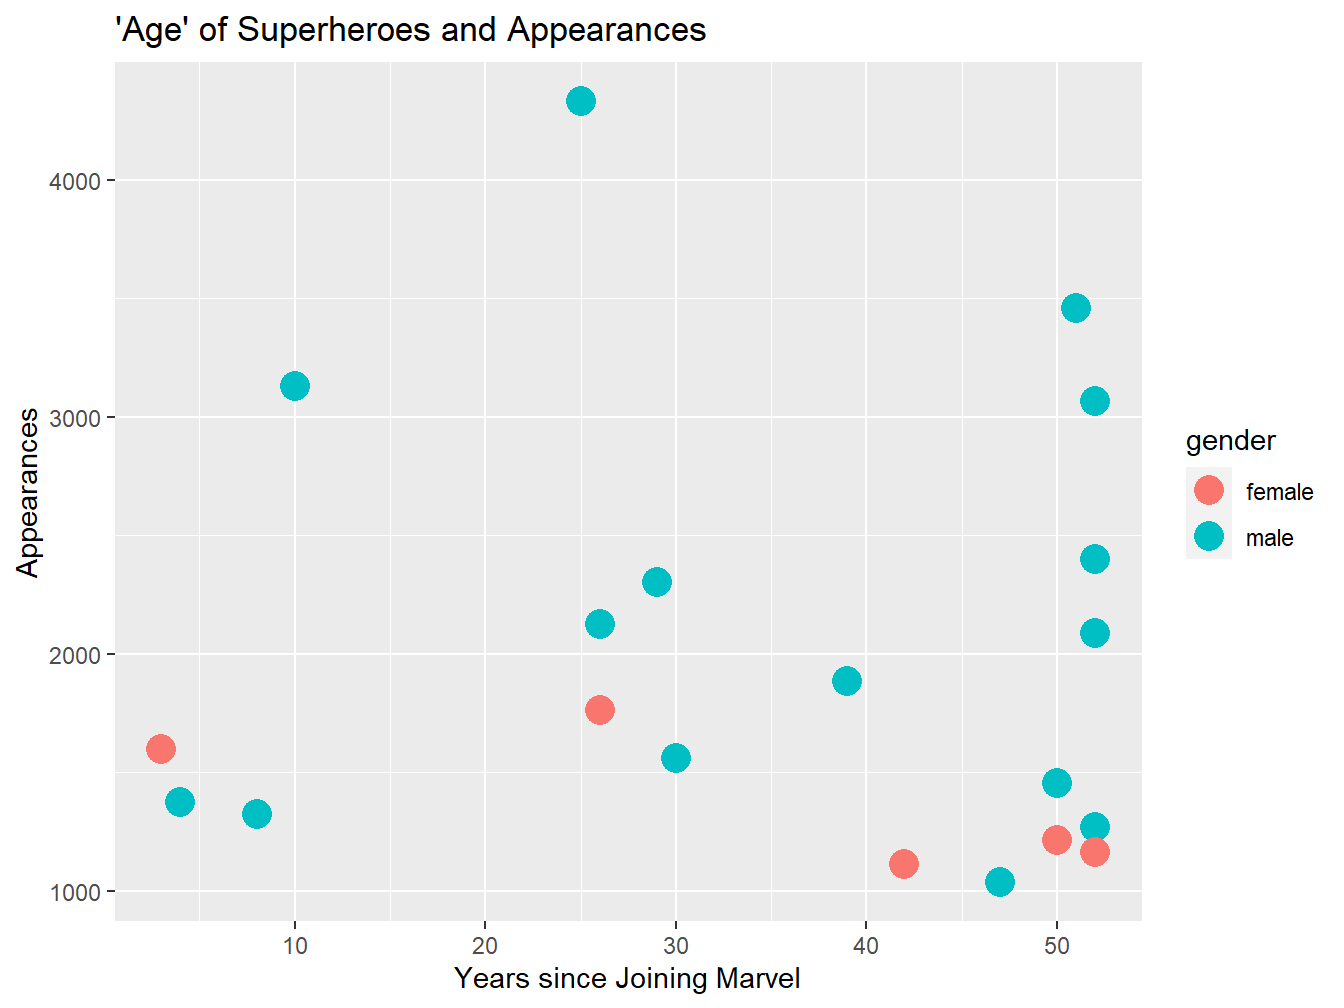
\includegraphics[width=0.8\linewidth]{famousdistrib_files/figure-latex/avengers-plot-1} 

}

\caption{Basic Avengers scatterplot}\label{fig:avengers-plot}
\end{figure}

We used two arguments in the ggplot function: data and mapping. Next, we added the geometry \texttt{geom\_point} using a plus sign (+). The aesthetic mapping in the ggplot function are then passed onto \texttt{geom\_point}.

Even though we must include data and mappings to produce a visualization, we do not always have to name the arguments themselves. For instance, we could simply write:

\begin{Shaded}
\begin{Highlighting}[]
\FunctionTok{ggplot}\NormalTok{(avengers, }\FunctionTok{aes}\NormalTok{(}\AttributeTok{x =}\NormalTok{ years\_since\_joining,}
                     \AttributeTok{y =}\NormalTok{ appearances,}
                     \AttributeTok{color =}\NormalTok{ gender)) }\SpecialCharTok{+}
  \FunctionTok{geom\_point}\NormalTok{()}
\end{Highlighting}
\end{Shaded}

Aesthetic mappings can also produce different geometries by simply changing the function. For example, instead of using \texttt{geom\_point} we can use \texttt{geom\_rect} to draw rectangles or squares.

\begin{Shaded}
\begin{Highlighting}[]
\FunctionTok{ggplot}\NormalTok{(avengers, }\FunctionTok{aes}\NormalTok{(}\AttributeTok{x =}\NormalTok{ years\_since\_joining,}
                     \AttributeTok{y =}\NormalTok{ appearances,}
                     \AttributeTok{fill =}\NormalTok{ gender)) }\SpecialCharTok{+}
  \FunctionTok{geom\_rect}\NormalTok{(}\FunctionTok{aes}\NormalTok{(}\AttributeTok{xmin =}\NormalTok{ years\_since\_joining }\SpecialCharTok{{-}} \DecValTok{1}\NormalTok{,}
                \AttributeTok{xmax =}\NormalTok{ years\_since\_joining }\SpecialCharTok{+} \DecValTok{1}\NormalTok{,}
                \AttributeTok{ymin =}\NormalTok{ appearances }\SpecialCharTok{{-}} \DecValTok{100}\NormalTok{,}
                \AttributeTok{ymax =}\NormalTok{ appearances }\SpecialCharTok{+} \DecValTok{100}\NormalTok{)) }\SpecialCharTok{+}
    \FunctionTok{labs}\NormalTok{(}\AttributeTok{title =} \StringTok{"\textquotesingle{}Age\textquotesingle{} of Superheroes and Appearances"}\NormalTok{,}
       \AttributeTok{x =} \StringTok{"Years since Joining Marvel"}\NormalTok{,}
       \AttributeTok{y =} \StringTok{"Appearances"}\NormalTok{)}
\end{Highlighting}
\end{Shaded}

\begin{figure}

{\centering 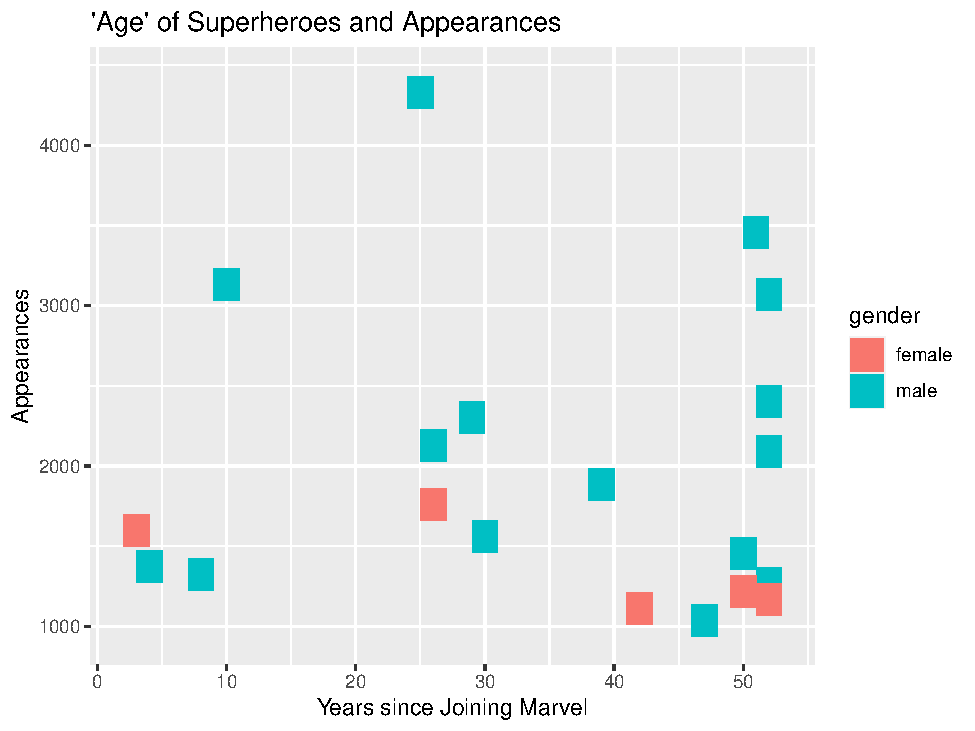
\includegraphics[width=0.8\linewidth]{famousdistrib_files/figure-latex/avengersplot-rect-1} 

}

\caption{Avengers scatterplot with rectangles}\label{fig:avengersplot-rect}
\end{figure}

Notice in Figure \ref{fig:avengersplot-rect} that the \texttt{geom\_rect} geometry requires aesthetic mappings beyond those in \texttt{geom\_point}, including the minimums and maximums for x and y. The color aesthetic of \texttt{geom\_point} turns to fill in \texttt{geom\_rect} since the rectangles are not points; they are shapes with empty space.

So far we have established that aesthetics can be passed onto different geometries.

Figure \ref{fig:ggplot-diagram} recaps where we are at now.

\begin{figure}

{\centering 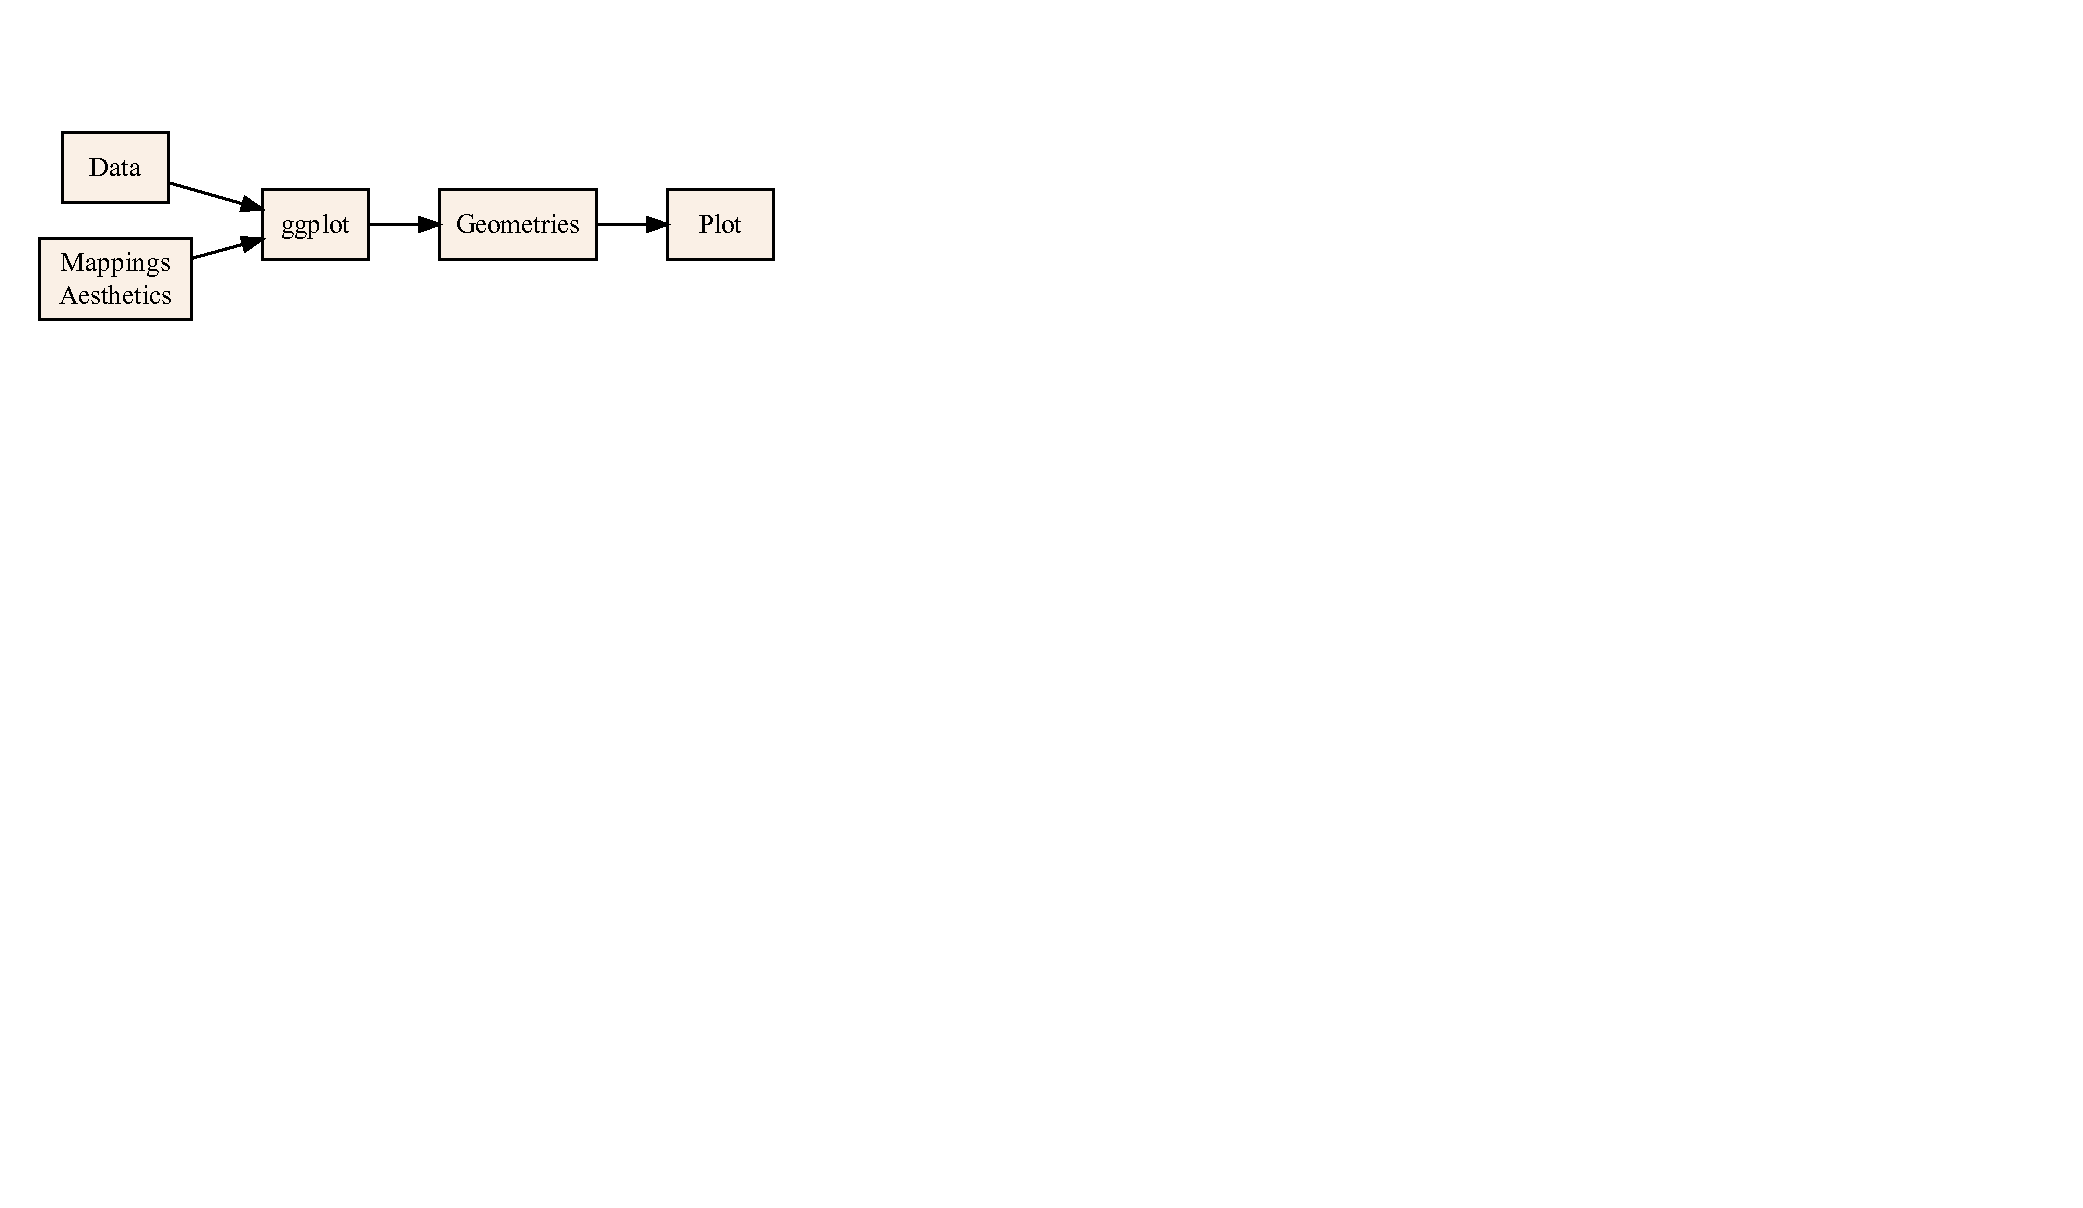
\includegraphics[width=0.8\linewidth]{famousdistrib_files/figure-latex/ggplot-diagram-1} 

}

\caption{ggplot diagram}\label{fig:ggplot-diagram}
\end{figure}

Generally, we want to provide mappings to the ggplot function so that they pass to all of our geometries. Including them in every line of code would be repetitive.

\begin{Shaded}
\begin{Highlighting}[]
\CommentTok{\# Don\textquotesingle{}t do this!}
\FunctionTok{ggplot}\NormalTok{(avengers, }\FunctionTok{aes}\NormalTok{(}\AttributeTok{x =}\NormalTok{ years\_since\_joining,}
                     \AttributeTok{y =}\NormalTok{ appearances,}
                     \AttributeTok{color =}\NormalTok{ gender)) }\SpecialCharTok{+}
  \FunctionTok{geom\_point}\NormalTok{(}\FunctionTok{aes}\NormalTok{(}\AttributeTok{x =}\NormalTok{ years\_since\_joining,}
                 \AttributeTok{y =}\NormalTok{ appearances,}
                 \AttributeTok{color =}\NormalTok{ gender))}

\CommentTok{\# Do this instead!}
\FunctionTok{ggplot}\NormalTok{(avengers, }\FunctionTok{aes}\NormalTok{(}\AttributeTok{x =}\NormalTok{ years\_since\_joining,}
                     \AttributeTok{y =}\NormalTok{ appearances,}
                     \AttributeTok{color =}\NormalTok{ gender)) }\SpecialCharTok{+}
  \FunctionTok{geom\_point}\NormalTok{()}
\end{Highlighting}
\end{Shaded}

But there are plenty of instances in which we wouldn't want to keep our aesthetics limited to the ggplot function line--for example, plots with two different groups or those with different scales on the y axis (although it is not generally recommended to have multiple scales on an axis since it is confusing). Let's return to the Avengers plot but keep the \texttt{color} argument in \texttt{geom\_point} so that the color of our text doesn't differ by gender.

\begin{Shaded}
\begin{Highlighting}[]
\FunctionTok{ggplot}\NormalTok{(avengers, }\FunctionTok{aes}\NormalTok{(}\AttributeTok{x =}\NormalTok{ years\_since\_joining, }\AttributeTok{y =}\NormalTok{ appearances)) }\SpecialCharTok{+}
  \FunctionTok{geom\_point}\NormalTok{(}\FunctionTok{aes}\NormalTok{(}\AttributeTok{color =}\NormalTok{ gender), }\AttributeTok{size =} \DecValTok{5}\NormalTok{) }\SpecialCharTok{+}
  \FunctionTok{geom\_text}\NormalTok{(}\FunctionTok{aes}\NormalTok{(}\AttributeTok{label =}\NormalTok{ name\_alias), }\AttributeTok{size =} \DecValTok{3}\NormalTok{) }\SpecialCharTok{+}
  \FunctionTok{labs}\NormalTok{(}\AttributeTok{title =} \StringTok{"\textquotesingle{}Age\textquotesingle{} of Superheroes and Appearances"}\NormalTok{,}
       \AttributeTok{x =} \StringTok{"Years since Joining Marvel"}\NormalTok{,}
       \AttributeTok{y =} \StringTok{"Appearances"}\NormalTok{)}
\end{Highlighting}
\end{Shaded}

\begin{figure}

{\centering 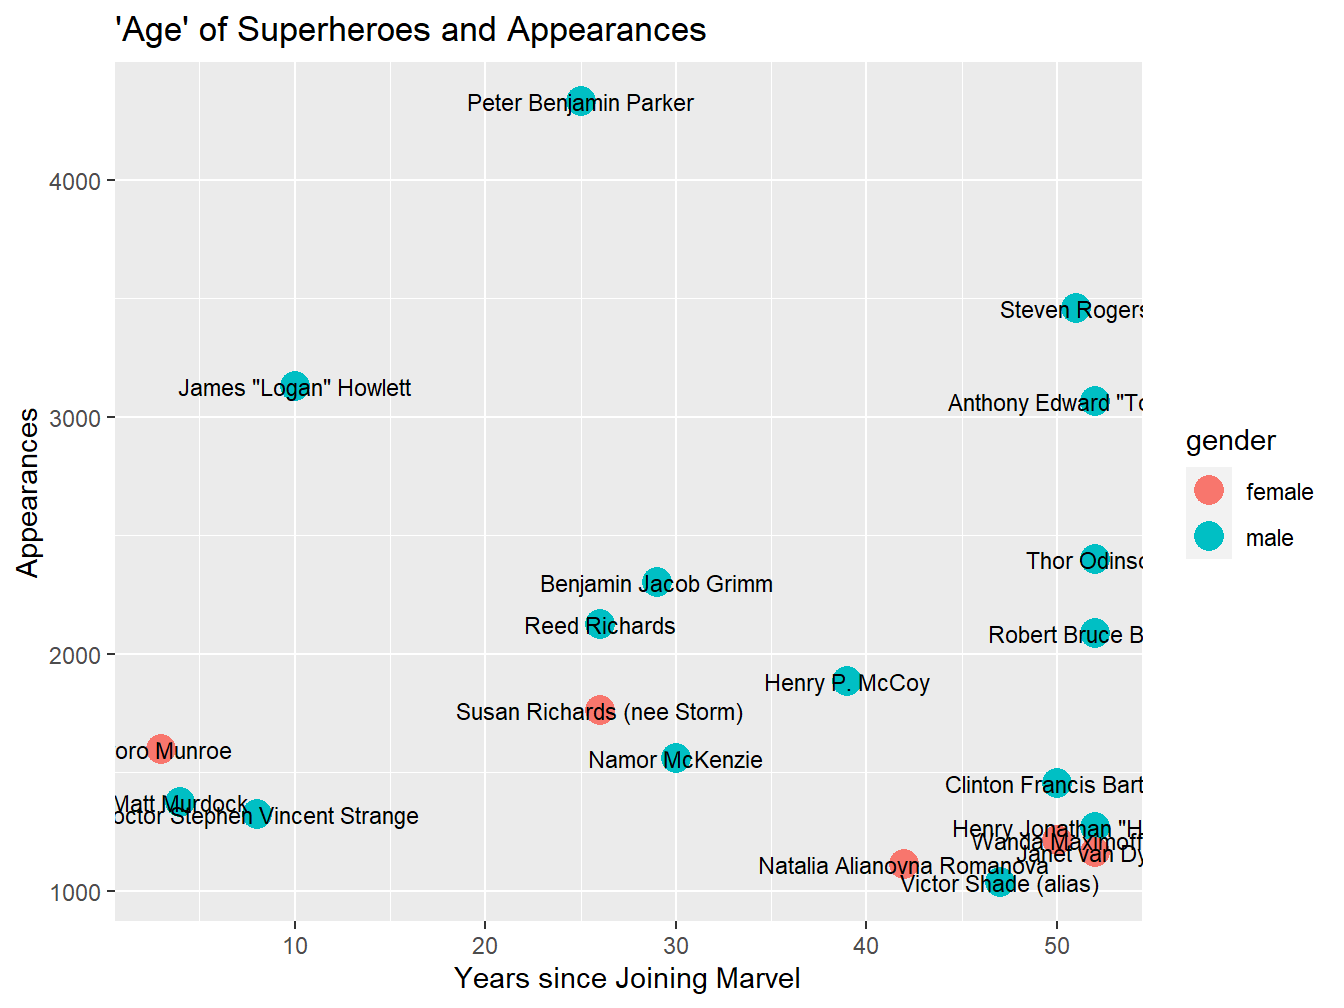
\includegraphics[width=0.8\linewidth]{famousdistrib_files/figure-latex/avengersplot-gender-1} 

}

\caption{Avengers scatterplot with unique color and label aesthetic assignments}\label{fig:avengersplot-gender}
\end{figure}

Figure \ref{fig:avengersplot-gender} doesn't look pretty but you get the idea. A general rule to follow with data visualizations is to avoid mapping one aesthetic to multiple variables. For instance, a plot in which the color is used to illustrate both an Avenger's gender and their name would be confusing.

\begin{Shaded}
\begin{Highlighting}[]
\CommentTok{\# Don\textquotesingle{}t do this!}
\FunctionTok{ggplot}\NormalTok{(avengers, }\FunctionTok{aes}\NormalTok{(}\AttributeTok{x =}\NormalTok{ years\_since\_joining, }\AttributeTok{y =}\NormalTok{ appearances)) }\SpecialCharTok{+}
  \FunctionTok{geom\_point}\NormalTok{(}\FunctionTok{aes}\NormalTok{(}\AttributeTok{color =}\NormalTok{ gender), }\AttributeTok{size =} \DecValTok{5}\NormalTok{) }\SpecialCharTok{+}
  \FunctionTok{geom\_text}\NormalTok{(}\FunctionTok{aes}\NormalTok{(}\AttributeTok{color =}\NormalTok{ name\_alias, }\AttributeTok{label =}\NormalTok{ name\_alias), }\AttributeTok{size =} \DecValTok{3}\NormalTok{) }\SpecialCharTok{+}
  \FunctionTok{labs}\NormalTok{(}\AttributeTok{title =} \StringTok{"\textquotesingle{}Age\textquotesingle{} of Superheroes and Appearances"}\NormalTok{,}
       \AttributeTok{x =} \StringTok{"Years since Joining Marvel"}\NormalTok{,}
       \AttributeTok{y =} \StringTok{"Appearances"}\NormalTok{)}
\end{Highlighting}
\end{Shaded}

\begin{figure}

{\centering 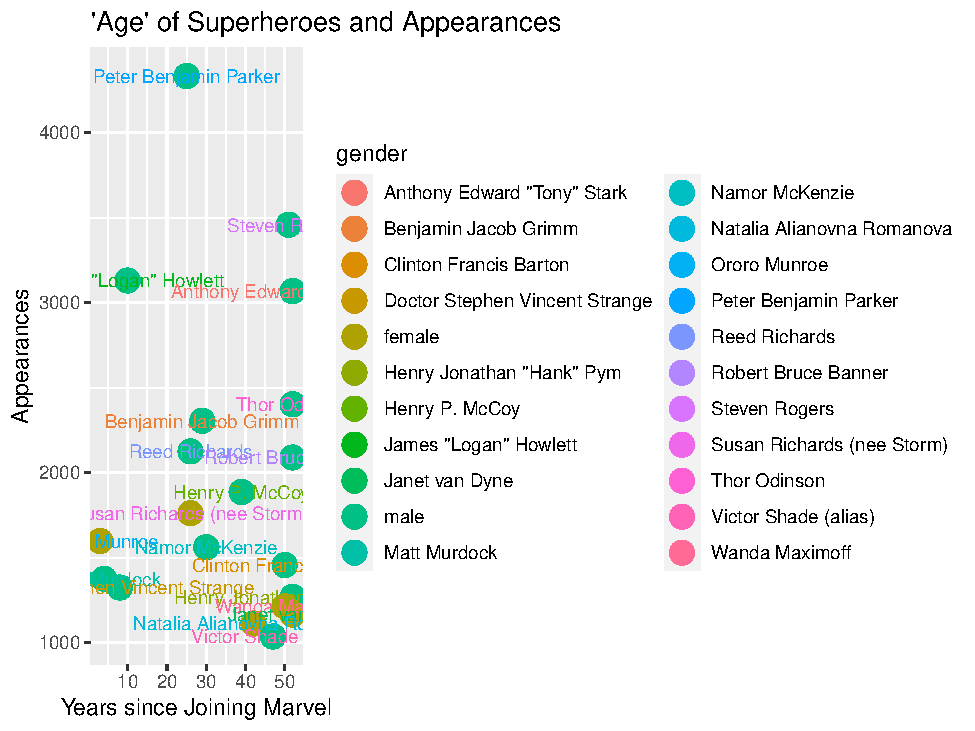
\includegraphics[width=0.8\linewidth]{famousdistrib_files/figure-latex/avengersplot-wrong-1} 

}

\caption{Incorrect Aesthetic Mapping}\label{fig:avengersplot-wrong}
\end{figure}

Sadly, Steve Rogers is not a gender and neither are the other Avenger names in the legend. This is why we should not map one aesthetic to more than one variable.

\hypertarget{altering-aesthetics-and-scalings}{%
\subsection{Altering Aesthetics and Scalings}\label{altering-aesthetics-and-scalings}}

Now, let's introduce a way to change our aesthetics further. There are some arguments within geom functions that allow us to do this. For instance, you might have noticed that I used \texttt{size} to make points and labels larger in the previous plots. We can also use \texttt{color} or \texttt{fill} to make adjustments to our geoms.

\begin{Shaded}
\begin{Highlighting}[]
\FunctionTok{ggplot}\NormalTok{(avengers, }\FunctionTok{aes}\NormalTok{(}\AttributeTok{x =}\NormalTok{ years\_since\_joining,}
                     \AttributeTok{y =}\NormalTok{ appearances)) }\SpecialCharTok{+}
  \FunctionTok{geom\_point}\NormalTok{(}\AttributeTok{color =} \StringTok{"tomato"}\NormalTok{, }\AttributeTok{size =} \DecValTok{5}\NormalTok{)}
\end{Highlighting}
\end{Shaded}

\begin{figure}

{\centering 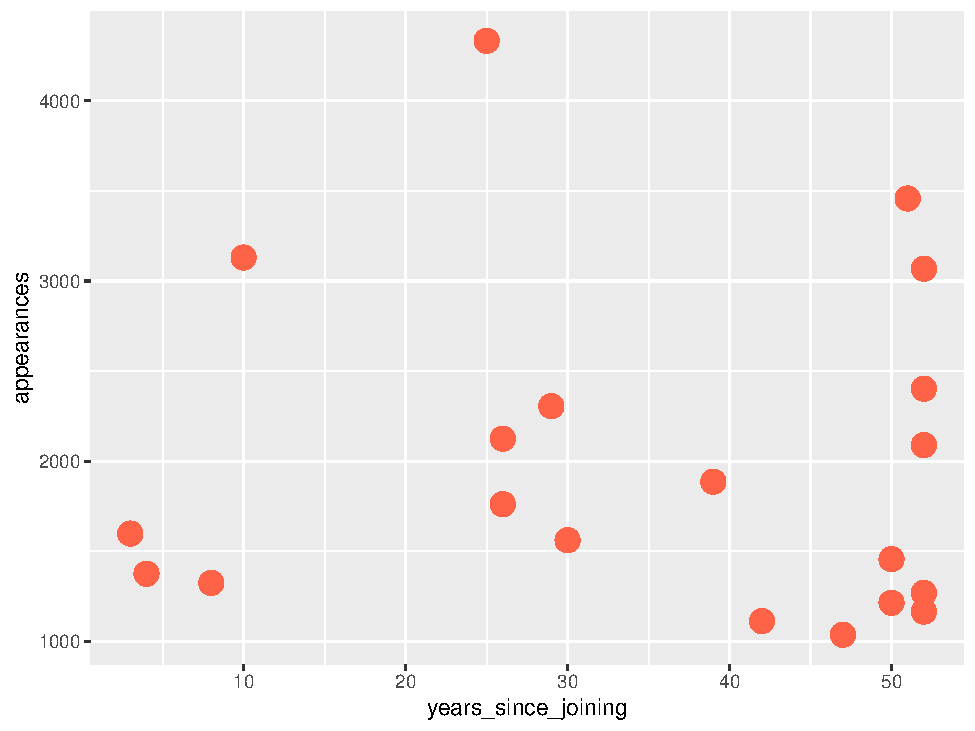
\includegraphics[width=0.8\linewidth]{famousdistrib_files/figure-latex/avengersplot-red-1} 

}

\caption{Avengers scatterplot in red!}\label{fig:avengersplot-red}
\end{figure}

But previously we have related color with an Avenger's gender. ggplot uses some default colors to differentiate male and female Avengers but we can change this further with \textbf{scales}. Every scale function has three components:

\begin{enumerate}
\def\labelenumi{\arabic{enumi}.}
\tightlist
\item
  \texttt{scale\_}
\item
  The name of the aesthetic we are scaling. In this case, \texttt{color}.
\item
  A method of applying the scale. In this case, we'll use \texttt{manual}.
\end{enumerate}

So to combine all of the previous steps together, we would call the function\texttt{scale\_color\_manual} to directly alter the colors of our aesthetic related to gender.

\begin{Shaded}
\begin{Highlighting}[]
\FunctionTok{ggplot}\NormalTok{(avengers, }\FunctionTok{aes}\NormalTok{(}\AttributeTok{x =}\NormalTok{ years\_since\_joining,}
                     \AttributeTok{y =}\NormalTok{ appearances,}
                     \AttributeTok{color =}\NormalTok{ gender)) }\SpecialCharTok{+}
  \FunctionTok{geom\_point}\NormalTok{(}\AttributeTok{size =} \DecValTok{5}\NormalTok{) }\SpecialCharTok{+}
  \FunctionTok{scale\_color\_manual}\NormalTok{(}\AttributeTok{values =} \FunctionTok{c}\NormalTok{(}\StringTok{"Tomato"}\NormalTok{, }\StringTok{"Navy"}\NormalTok{))}
\end{Highlighting}
\end{Shaded}

\textbackslash begin\{figure\}

\{\centering 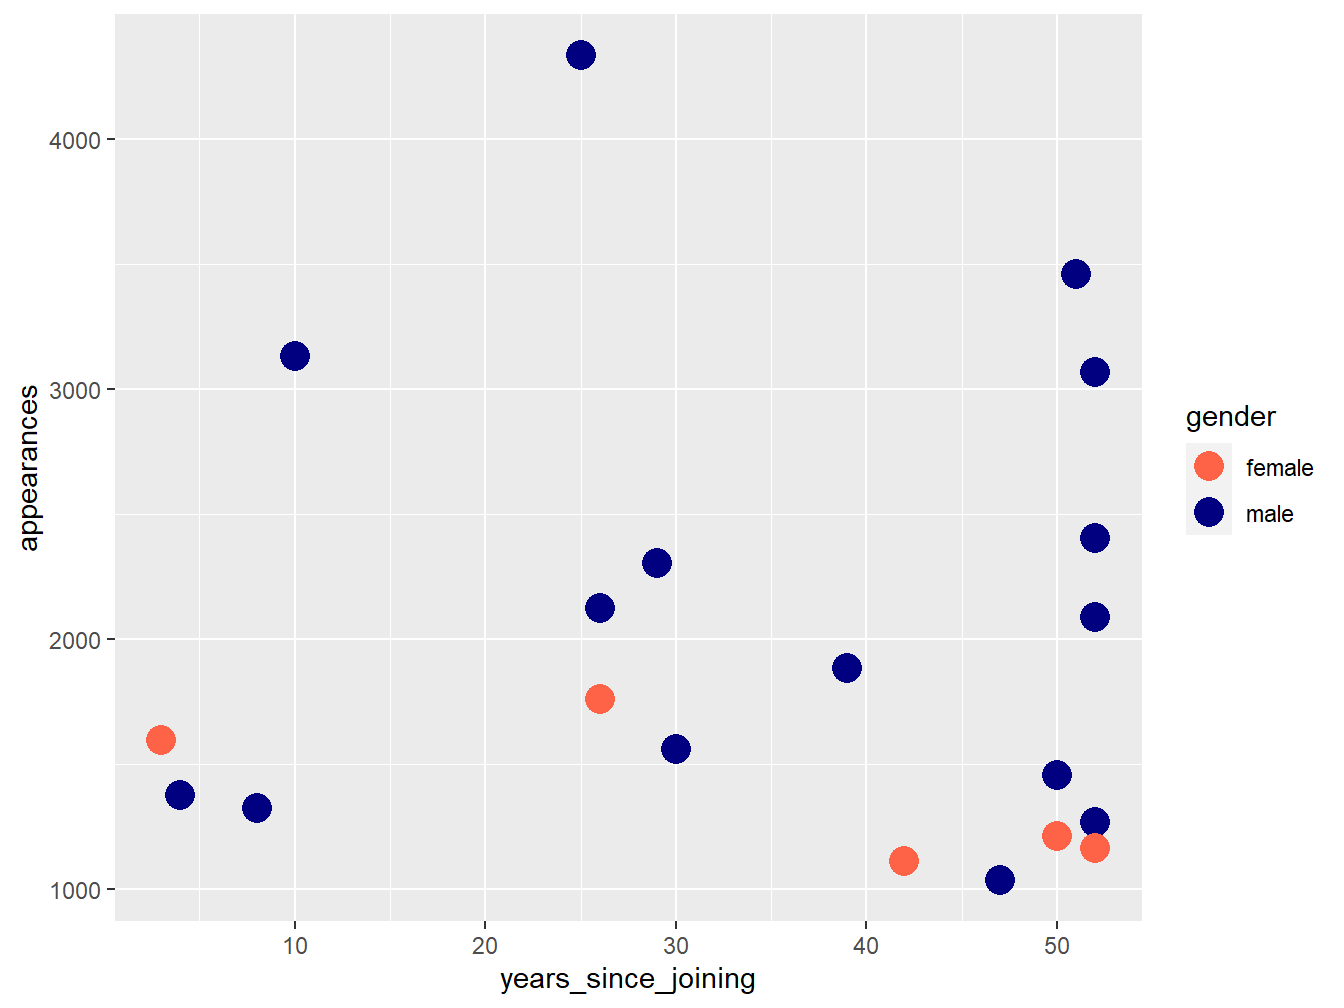
\includegraphics[width=0.8\linewidth]{famousdistrib_files/figure-latex/avengersplot-scale-1}

\}

\textbackslash caption\{Avengers scatterplot using \texttt{scale\_color\_manual}\}\label{fig:avengersplot-scale}
\textbackslash end\{figure\}

We've not only learned about the gender gap in the Marvel universe but also how to apply scales to our aesthetics! There are a number of scales that we can use further. For example, \texttt{scale\_alpha\_binned} allows us to alter the transparency of points after providing a \texttt{range} between 0-1. The \texttt{breaks} argument separates our observations into different groups.

\begin{Shaded}
\begin{Highlighting}[]
\FunctionTok{ggplot}\NormalTok{(avengers, }\FunctionTok{aes}\NormalTok{(}\AttributeTok{x =}\NormalTok{ years\_since\_joining,}
                     \AttributeTok{y =}\NormalTok{ appearances,}
                     \AttributeTok{alpha =}\NormalTok{ appearances)) }\SpecialCharTok{+}
  \FunctionTok{geom\_point}\NormalTok{(}\AttributeTok{size =} \DecValTok{5}\NormalTok{) }\SpecialCharTok{+}
  \FunctionTok{scale\_alpha\_continuous}\NormalTok{(}\AttributeTok{range =} \FunctionTok{c}\NormalTok{(}\FloatTok{0.2}\NormalTok{, }\DecValTok{1}\NormalTok{),}
                         \AttributeTok{breaks =} \FunctionTok{c}\NormalTok{(}\DecValTok{2000}\NormalTok{, }\DecValTok{3000}\NormalTok{, }\DecValTok{4000}\NormalTok{))}
\end{Highlighting}
\end{Shaded}

\textbackslash begin\{figure\}

\{\centering 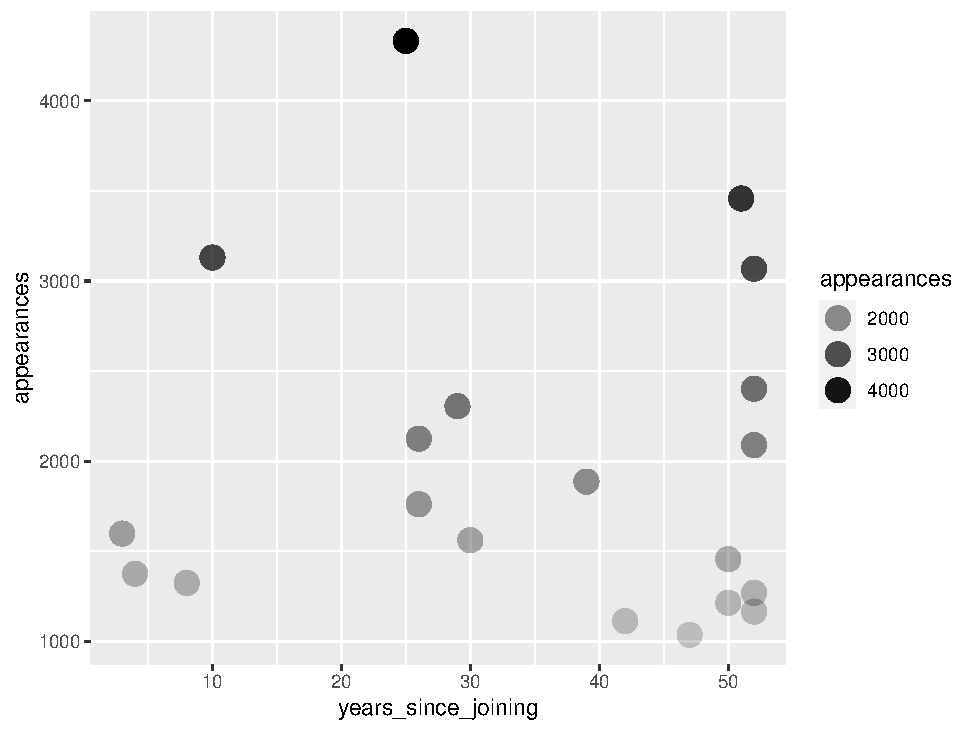
\includegraphics[width=0.8\linewidth]{famousdistrib_files/figure-latex/avengersplot-alpha-1}

\}

\textbackslash caption\{Avengers scatterplot with \texttt{scale\_alpha\_continuous}\}\label{fig:avengersplot-alpha}
\textbackslash end\{figure\}

An important fact to remember is that mapping a variable to more than one aesthetic sometimes exaggerate differences in data. In this case, using two aesthetics--y and alpha--for appearance count draws the eye to the Avengers with the most appearances. This is why any data scientist must consider the \href{https://socviz.co/index.html\#preface}{principles of data visualization} and how certain techniques mislead or distort data.

So far, we have learned how to call the \texttt{ggplot} function, apply aesthetic mappings, layer geometries, and alter aesthetics with scales. Any data visualization, regardless of its complexity, follows this formula.

Hopefully this chapter has provided you a some more confidence as you begin producing your own visualizations. However, this is by no means an exhaustive tutorial. To learn more about data visualizations here are some useful resources:

\begin{itemize}
\tightlist
\item
  \href{https://www.amazon.com/gp/product/0596809158/ref=as_li_tf_tl?ie=UTF8\&camp=1789\&creative=9325\&creativeASIN=0596809158\&linkCode=as2\&tag=cooforr09-20}{R Cookbook}
\item
  \href{http://www.cookbook-r.com/}{Cookbook for R}
\item
  \href{https://www.r-graph-gallery.com/index.html}{The R Graph Gallery}
\item
  \href{https://www.rfordatasci.com/}{R for Data Science Online Community}
\end{itemize}

The rest of this guide specifically uses our new visualization tool to learn about the statistical distributions that govern our world. Click on to learn more!

\hypertarget{Distributions}{%
\section{Understanding Distributions}\label{Distributions}}

Every distribution discovered in the probability world is determined by a \textbf{random variable}. These variables are the not the same ones that you were exposed to in algebra or calculus class. Instead, they are used to map random processes, like rolling dice or playing the lottery, to readable notation.

We'll begin with a simple example of this by flipping a coin. Let the random variable X (usually random variables are capital letters) denote this process. It can take two forms, heads or tails. We can use a binary 0 or 1 to show this:

\[X = \{0,1\}\]

You might be asking yourself: ``What does this have to do with probability?'' We begin by defining the random variable so that we can later discover its mathematical attributes, such as its mean or variance, for example.

We can also define the probability that the random variable \(X\) (the coin) takes the form of heads or tails by using probability notation.

\[P(X = x)\]

Where x can equal 0 or 1. We can interpret the statement above as ``the probability that the random variable X equals x.'' So what is that probability? By common sense, we can conclude that the probability that you get heads is \(P(X=1)=1/2\). We can extend this logic to show that \textbf{the sum of probabilities for any random variable is 1}.

\[P(X = 0) + P(X = 1)= 1/2 + 1/2 = 1\]

In other, more complicated probability distributions, we use random variables such as \(X\) to mark these processes without having to explain them each time.

\hypertarget{Uniform}{%
\subsection{Uniform Distribution}\label{Uniform}}

We'll begin our journey with uniform distribution. Given \(a < b\), we can define this distribution's \textbf{density} as:

\[ P(X=x) = \frac{1}{b-a}\quad \textrm{for} \enspace a \leq x \leq b \]

When we refer to densities we are talking about probabilities. The two terms are interchangeable, but the term \textbf{density} emphasizes the finite probability space that a distribution occupies. As mentioned previously, the sum of probabilities for any distribution is 1.

How do we get this equation? Imagine drawing a rectangle in the interval (a,b) with height 1/(b-a) as in Figure \ref{fig:uniform-basic}.

\begin{Shaded}
\begin{Highlighting}[]
\FunctionTok{ggplot}\NormalTok{() }\SpecialCharTok{+}
  \FunctionTok{geom\_rect}\NormalTok{(}\FunctionTok{aes}\NormalTok{(}\AttributeTok{xmin =} \DecValTok{0}\NormalTok{, }\AttributeTok{xmax =} \DecValTok{1}\NormalTok{, }\AttributeTok{ymin =} \DecValTok{0}\NormalTok{, }\AttributeTok{ymax =} \DecValTok{1}\NormalTok{), }
            \AttributeTok{fill =} \ConstantTok{NA}\NormalTok{,}
            \AttributeTok{color =} \StringTok{"black"}\NormalTok{) }\SpecialCharTok{+}
  \FunctionTok{labs}\NormalTok{(}\AttributeTok{x =} \StringTok{"x"}\NormalTok{, }\AttributeTok{y =} \StringTok{"Density"}\NormalTok{) }\SpecialCharTok{+}
  \FunctionTok{scale\_x\_continuous}\NormalTok{(}\AttributeTok{breaks =} \FunctionTok{c}\NormalTok{(}\DecValTok{0}\NormalTok{,}\DecValTok{1}\NormalTok{), }\AttributeTok{labels =} \FunctionTok{c}\NormalTok{(}\StringTok{"a"}\NormalTok{, }\StringTok{"b"}\NormalTok{)) }\SpecialCharTok{+}
  \FunctionTok{scale\_y\_continuous}\NormalTok{(}\AttributeTok{breaks =} \FunctionTok{c}\NormalTok{(}\DecValTok{0}\NormalTok{,}\DecValTok{1}\NormalTok{), }\AttributeTok{labels =} \FunctionTok{c}\NormalTok{(}\StringTok{""}\NormalTok{, }\StringTok{"h"}\NormalTok{))}
\end{Highlighting}
\end{Shaded}

\begin{figure}

{\centering 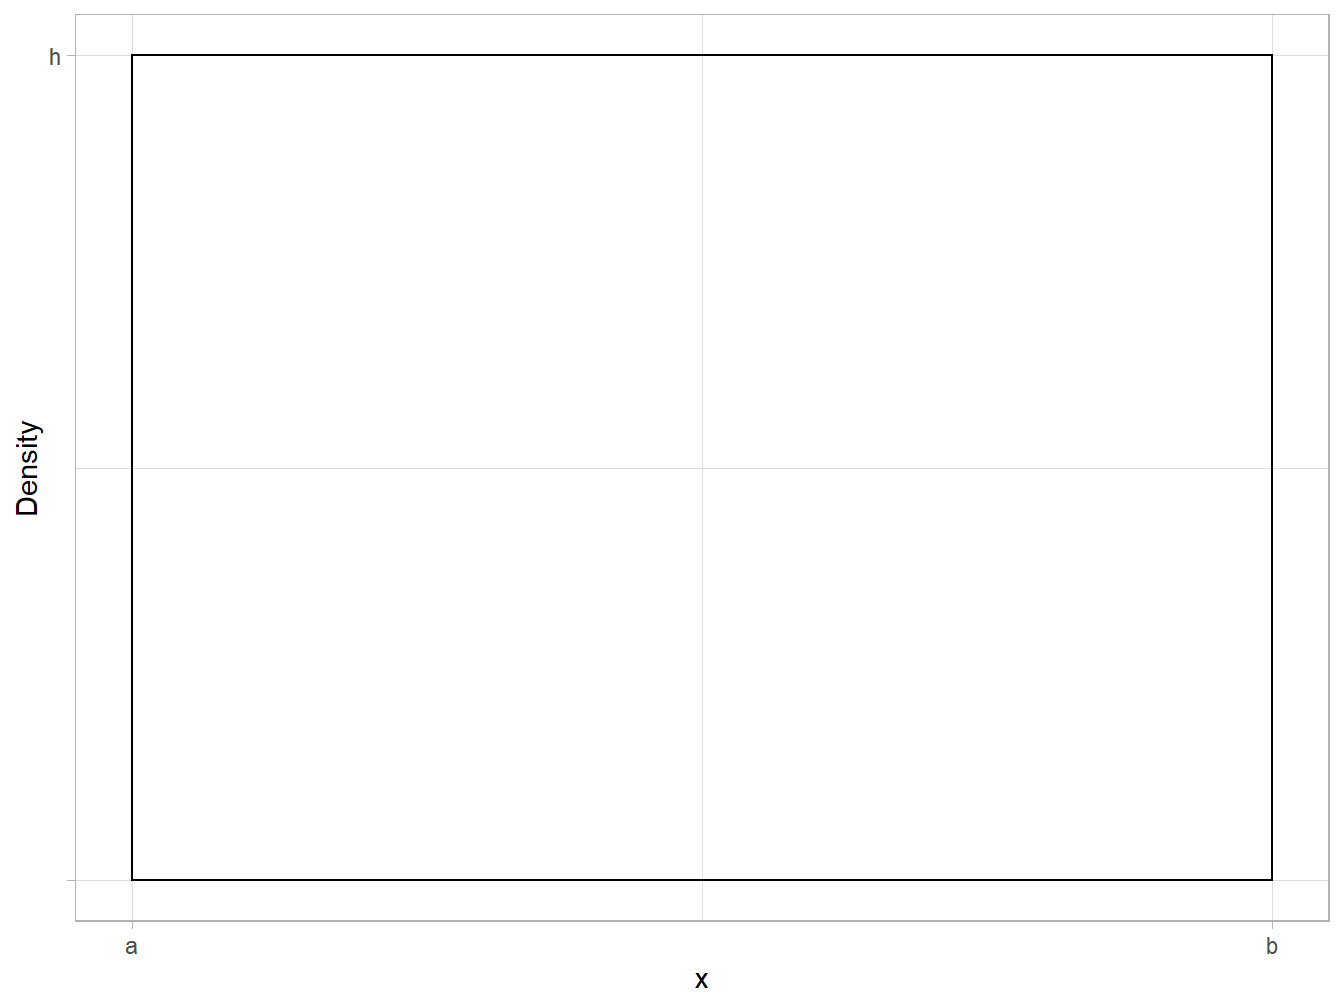
\includegraphics[width=0.8\linewidth]{famousdistrib_files/figure-latex/uniform-basic-1} 

}

\caption{Remember Scales? See if you can understand the code}\label{fig:uniform-basic}
\end{figure}

We have the height as \(\frac{1}{(b-a)}\). We know this since the cumulative area of a distribution must be 1 and the width is b-a. Using the area of a rectangle with h being the height of the uniform distribution.

\[(b-a)h=1\]

For the equation to hold, h must equal 1/(b-a).

Let's define X as a \textbf{discrete} random variable that is uniform on 1 through 10. The term ``discrete'' means that \(X\) can only be integers, and the fact that its probabilities are uniform means that every integer has an equal probability of occurring. Therefore:

\[
\begin{split}
&X=\{1,2,...,10\}\\&P(X=x)=\frac{1}{10-1}=1/9\quad\textrm{for}\quad1\leq x\leq 10 
\end{split}
\]

The first line outlines the random variable X and the numbers that it can take. The second line then calculates the probability of the random variable taking the integers 1-10 as 1/9. In other words, the \textbf{density}, or individual probability, for each of \(1\leq x\leq 10\) is 1/9.

The first \texttt{stats} function we can use with the uniform distribution is \texttt{dunif} which also returns the density at point x in the distribution given left and right bounds. This is quite easy to determine in the uniform distribution because \textbf{every point has the same density of h}- in other words, the height. \texttt{dunif} has 3 arguments.

\begin{enumerate}
\def\labelenumi{\arabic{enumi}.}
\item
  A vector of values to calculate densities for.
\item
  The minimum or \texttt{min} of the distribution.
\item
  The maximum or \texttt{max} of the distribution.
\end{enumerate}

We'll return to our example where the beginning and end of the uniform distribution is at x = 1 and x = 10, respectively. What are the densities at x = 1, 5, and 10?

\begin{Shaded}
\begin{Highlighting}[]
\FunctionTok{dunif}\NormalTok{(}\FunctionTok{c}\NormalTok{(}\DecValTok{1}\NormalTok{, }\DecValTok{5}\NormalTok{, }\DecValTok{10}\NormalTok{), }\AttributeTok{min =} \DecValTok{1}\NormalTok{, }\AttributeTok{max =} \DecValTok{10}\NormalTok{)}
\end{Highlighting}
\end{Shaded}

\begin{verbatim}
## [1] 0.1111111 0.1111111 0.1111111
\end{verbatim}

You are correct if you guessed 1/9 or approximately 0.111! If \(a = 1\), \(b = 10\) then by definition \(h = 1/9\). Thus, as we calculated earlier, every point in the distribution has a density of 1/9.

We can visualize this by drawing a rectangle using \texttt{geom\_rect} and then adding points with \texttt{geom\_point}. Remember that certain geometries require aesthetics beyond x and y.

\begin{Shaded}
\begin{Highlighting}[]
\FunctionTok{ggplot}\NormalTok{() }\SpecialCharTok{+}
  \FunctionTok{geom\_rect}\NormalTok{(}\FunctionTok{aes}\NormalTok{(}\AttributeTok{xmin =} \DecValTok{1}\NormalTok{, }\AttributeTok{xmax =} \DecValTok{10}\NormalTok{, }\AttributeTok{ymin =} \DecValTok{0}\NormalTok{, }\AttributeTok{ymax =} \DecValTok{1}\NormalTok{), }\AttributeTok{fill =} \ConstantTok{NA}\NormalTok{, }
            \AttributeTok{color =} \StringTok{"black"}\NormalTok{) }\SpecialCharTok{+}
  \FunctionTok{labs}\NormalTok{(}\AttributeTok{x =} \StringTok{"x"}\NormalTok{, }\AttributeTok{y =} \StringTok{"Density"}\NormalTok{) }\SpecialCharTok{+}
  \FunctionTok{geom\_point}\NormalTok{(}\FunctionTok{aes}\NormalTok{(}\AttributeTok{x =} \FunctionTok{c}\NormalTok{(}\DecValTok{1}\NormalTok{, }\DecValTok{5}\NormalTok{, }\DecValTok{10}\NormalTok{), }\AttributeTok{y =} \DecValTok{1}\NormalTok{), }\AttributeTok{size =} \DecValTok{5}\NormalTok{, }\AttributeTok{color =} \StringTok{"navy"}\NormalTok{)}
\end{Highlighting}
\end{Shaded}

\begin{figure}

{\centering 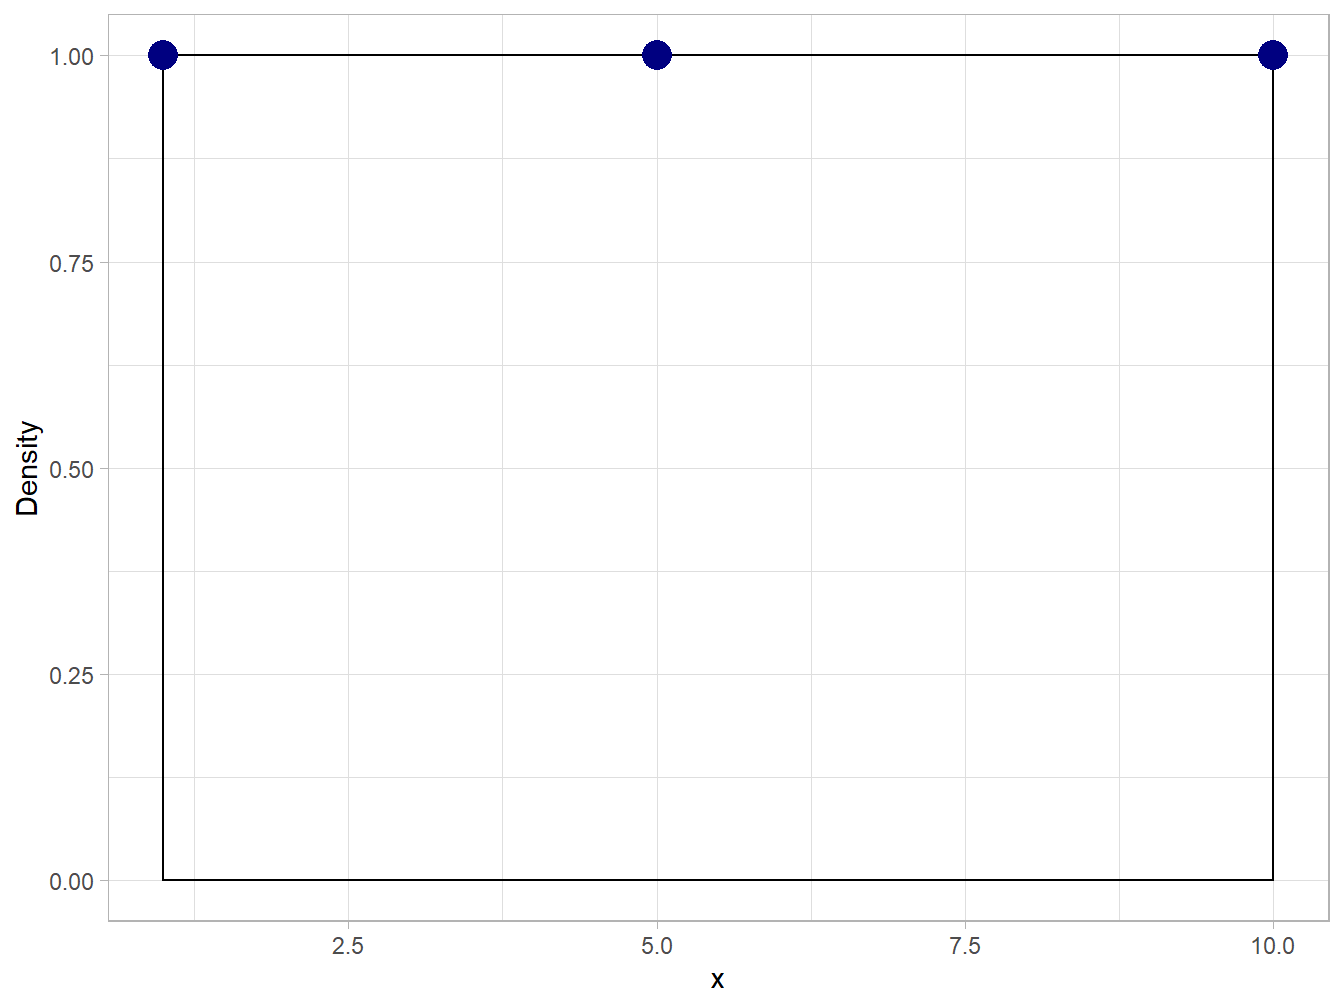
\includegraphics[width=0.8\linewidth]{famousdistrib_files/figure-latex/geomrect-plot-1} 

}

\caption{Uniform distribution with marked densities}\label{fig:geomrect-plot}
\end{figure}

The \texttt{punif()} function helps us find the cumulative density between at the qth quantile. Using a different rectangle with \(a = 0\), \(b = 4\), and \(h = 1/4\), we can find the proportion of the distribution between the minimum of 0 and maximum of 2 by writing the following:

\begin{Shaded}
\begin{Highlighting}[]
\FunctionTok{punif}\NormalTok{(}\DecValTok{2}\NormalTok{, }\DecValTok{0}\NormalTok{, }\DecValTok{4}\NormalTok{, }\AttributeTok{lower.tail =} \ConstantTok{TRUE}\NormalTok{) }\CommentTok{\# Remember: we don\textquotesingle{}t always have to name our arguments if we know the order.}
\end{Highlighting}
\end{Shaded}

\begin{verbatim}
## [1] 0.5
\end{verbatim}

We can similarly write:

\begin{Shaded}
\begin{Highlighting}[]
\FunctionTok{sum}\NormalTok{(}\FunctionTok{dunif}\NormalTok{(}\DecValTok{0}\SpecialCharTok{:}\DecValTok{1}\NormalTok{, }\AttributeTok{min =} \DecValTok{0}\NormalTok{, }\AttributeTok{max =} \DecValTok{4}\NormalTok{)) }\CommentTok{\# Not including 2.}
\end{Highlighting}
\end{Shaded}

\begin{verbatim}
## [1] 0.5
\end{verbatim}

There are three arguments in this function: a vector of quantiles, a minimum, maximum, and a binary \texttt{lower.tail} argument. By default this is set to \texttt{TRUE}.

We can also think about the \texttt{punif()} function as drawing a smaller rectangle from 0 to 2 (if \texttt{lower.tail\ =\ FALSE}) and calculating its area. Below, this is the same as the percent of the total area that the navy rectangle occupies.

\begin{Shaded}
\begin{Highlighting}[]
\FunctionTok{ggplot}\NormalTok{() }\SpecialCharTok{+}
  \FunctionTok{geom\_rect}\NormalTok{(}\FunctionTok{aes}\NormalTok{(}\AttributeTok{xmin =} \DecValTok{0}\NormalTok{, }\AttributeTok{xmax =} \DecValTok{2}\NormalTok{, }\AttributeTok{ymin =} \DecValTok{0}\NormalTok{, }\AttributeTok{ymax =} \DecValTok{1}\SpecialCharTok{/}\DecValTok{4}\NormalTok{),  }\CommentTok{\# Small rectangle}
            \AttributeTok{alpha =}\NormalTok{ .}\DecValTok{2}\NormalTok{, }
            \AttributeTok{fill =} \StringTok{"navy"}\NormalTok{, }
            \AttributeTok{color =} \StringTok{"navy"}\NormalTok{, }
            \AttributeTok{linetype =} \StringTok{"dashed"}\NormalTok{) }\SpecialCharTok{+}
    \FunctionTok{geom\_rect}\NormalTok{(}\FunctionTok{aes}\NormalTok{(}\AttributeTok{xmin =} \DecValTok{0}\NormalTok{, }\AttributeTok{xmax =} \DecValTok{4}\NormalTok{, }\AttributeTok{ymin =} \DecValTok{0}\NormalTok{, }\AttributeTok{ymax =} \DecValTok{1}\SpecialCharTok{/}\DecValTok{4}\NormalTok{), }\CommentTok{\# Large rectangle}
              \AttributeTok{fill =} \ConstantTok{NA}\NormalTok{, }
              \AttributeTok{color =} \StringTok{"black"}\NormalTok{) }\SpecialCharTok{+}
  \FunctionTok{labs}\NormalTok{(}\AttributeTok{x =} \StringTok{"x"}\NormalTok{, }\AttributeTok{y =} \StringTok{"Density"}\NormalTok{)}
\end{Highlighting}
\end{Shaded}

\begin{figure}

{\centering 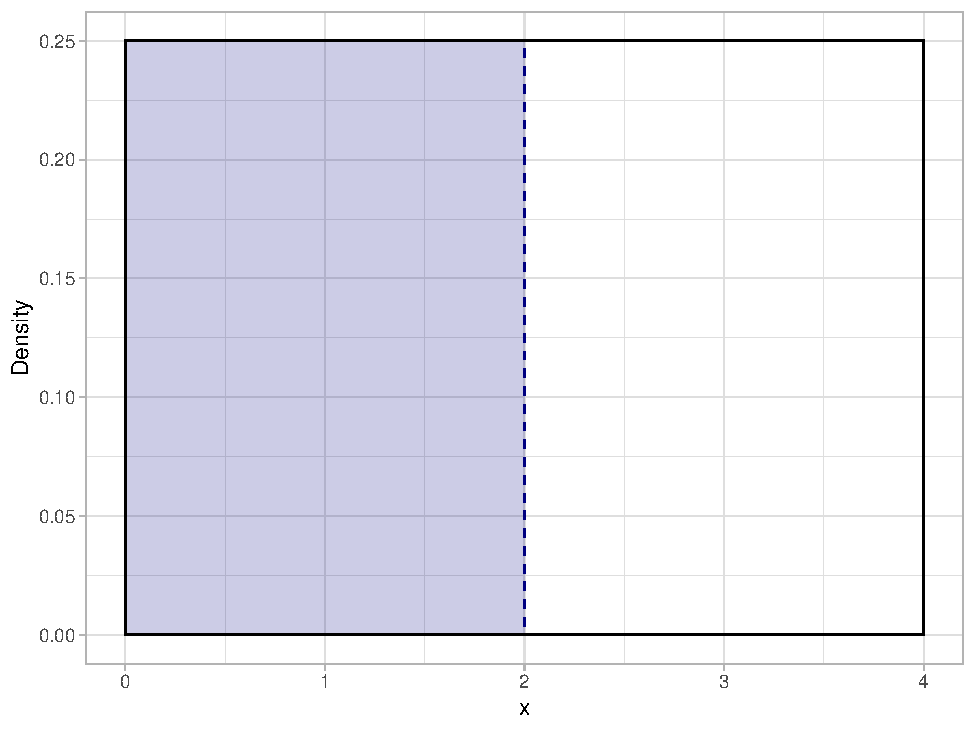
\includegraphics[width=0.8\linewidth]{famousdistrib_files/figure-latex/punif-plot-1} 

}

\caption{Uniform distribution with cumulative density marked}\label{fig:punif-plot}
\end{figure}

\[ area \hspace{0.2 cm}= \hspace{0.2 cm}base \hspace{0.2cm} * \hspace{0.2 cm}height\]

\[area = 2*0.25=0.5\]

Now we will consider the opposite scenario where we want to find the x-value that corresponds with the 50th percentile of our distribution. This is the purpose of \texttt{qunif()}. We already know from using the distribution function \texttt{punif()} that this is 2.

\begin{Shaded}
\begin{Highlighting}[]
\FunctionTok{qunif}\NormalTok{(}\FloatTok{0.5}\NormalTok{, }\DecValTok{0}\NormalTok{, }\DecValTok{4}\NormalTok{) }\CommentTok{\#lower.tail is also set to TRUE by default}
\end{Highlighting}
\end{Shaded}

\begin{verbatim}
## [1] 2
\end{verbatim}

The last function \texttt{runif()} generates random deviates within the distribution. There are three arguments in this function:

\begin{itemize}
\item
  n, the number of deviates we want to produce
\item
  min, the left bound of the uniform distribution
\item
  max, the right bound of the uniform distribution
\end{itemize}

We'll use the \texttt{round()} function to round them to the hundredths place.

\begin{Shaded}
\begin{Highlighting}[]
\CommentTok{\# Create object of deviates}

\NormalTok{unif\_dev }\OtherTok{\textless{}{-}} \FunctionTok{round}\NormalTok{(}\FunctionTok{runif}\NormalTok{(}\DecValTok{10}\NormalTok{, }\AttributeTok{min =} \DecValTok{0}\NormalTok{, }\AttributeTok{max =} \DecValTok{4}\NormalTok{), }\AttributeTok{digits =} \DecValTok{2}\NormalTok{)}

\CommentTok{\# Plot}

\FunctionTok{ggplot}\NormalTok{() }\SpecialCharTok{+}
  \FunctionTok{geom\_rect}\NormalTok{(}\FunctionTok{aes}\NormalTok{(}\AttributeTok{xmin =} \DecValTok{0}\NormalTok{, }\AttributeTok{xmax =} \DecValTok{4}\NormalTok{, }\AttributeTok{ymin =} \DecValTok{0}\NormalTok{, }\AttributeTok{ymax =} \DecValTok{1}\SpecialCharTok{/}\DecValTok{4}\NormalTok{), }
            \AttributeTok{fill =} \ConstantTok{NA}\NormalTok{,}
            \AttributeTok{color =} \StringTok{"black"}\NormalTok{) }\SpecialCharTok{+}
  \FunctionTok{geom\_point}\NormalTok{(}\FunctionTok{aes}\NormalTok{(}\AttributeTok{x =}\NormalTok{ unif\_dev, }\AttributeTok{y =} \DecValTok{1}\SpecialCharTok{/}\DecValTok{4}\NormalTok{), }\AttributeTok{size =} \DecValTok{5}\NormalTok{, }\AttributeTok{color =} \StringTok{"navy"}\NormalTok{) }\SpecialCharTok{+} \CommentTok{\# Plot deviates}
  \FunctionTok{labs}\NormalTok{(}\AttributeTok{x =} \StringTok{"x"}\NormalTok{, }\AttributeTok{y =} \StringTok{"Density"}\NormalTok{) }\SpecialCharTok{+}
  \FunctionTok{scale\_x\_continuous}\NormalTok{(}\AttributeTok{breaks =} \FunctionTok{seq}\NormalTok{(}\DecValTok{0}\NormalTok{, }\DecValTok{4}\NormalTok{, }\AttributeTok{by =} \DecValTok{1}\NormalTok{), }\AttributeTok{labels =} \FunctionTok{seq}\NormalTok{(}\DecValTok{0}\NormalTok{, }\DecValTok{4}\NormalTok{, }\AttributeTok{by =} \DecValTok{1}\NormalTok{))}
\end{Highlighting}
\end{Shaded}

\begin{figure}

{\centering 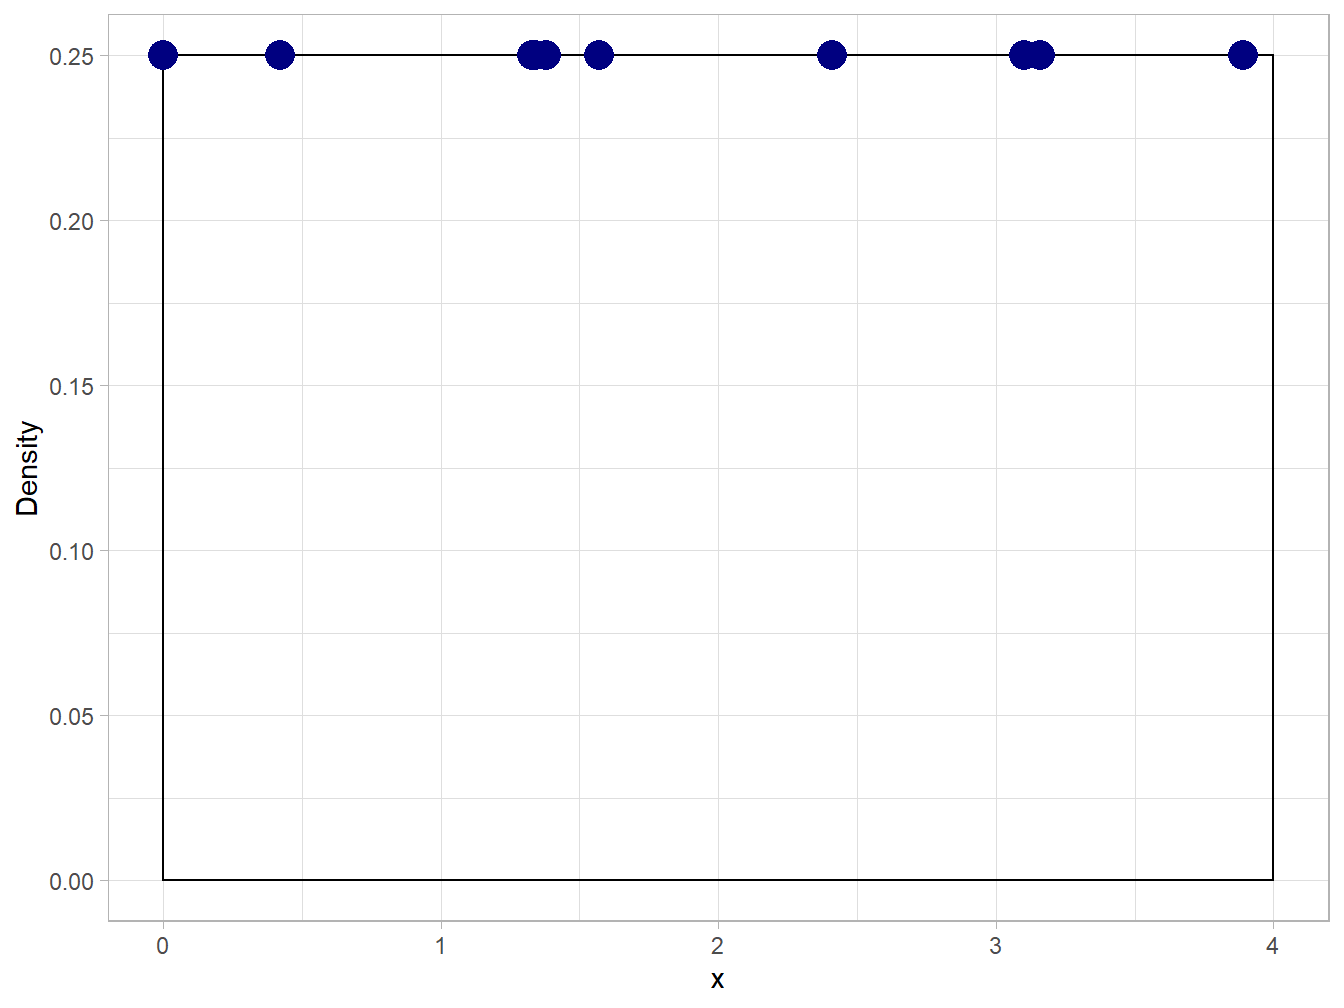
\includegraphics[width=0.8\linewidth]{famousdistrib_files/figure-latex/uniform-deviates-1} 

}

\caption{Uniform distribution with random deviates}\label{fig:uniform-deviates}
\end{figure}

The fact that the deviates appeared on non-integer values (i.e.~those that would normally be represented by fractions or decimals) reveals that the uniform distribution is not always discrete. In this case, as well as others later in this guide, distributions are labeled \textbf{continuous}. As we investigate several other types of distributions, we'll start with the discrete cases and then transition to the continuous ones.

\hypertarget{Discrete}{%
\section{Other Discrete Distributions}\label{Discrete}}

\hypertarget{Geometric}{%
\subsection{Geometric Distribution}\label{Geometric}}

For the next distribution, imagine a basketball player that is not particularly good. Whenever he takes a free throw, there is a 10\% probability that he makes it. How many free throws can we expect him to shoot before he makes one?

The geometric distribution helps us answer this question. We can think of this as a spread of \(N\) trials required to reach a probability \(p\) in the following equation.

\[P(N = n) = (1-p)^{n} p \hspace{0.7cm}for\hspace{0.2cm} n=0,1,...,\infty\]

Since trials can only be measured in integers, the geometric distribution is another \textbf{discrete} distribution.

Although there is a more in-depth proof, the formula for this distribution is already quite intuitive. First, the geometric distribution needs \(n\) failures and one success for \(N to equal n\). Likewise, if the probability of a success is represented by \(p\), the probability of a failure must be \(1-p\).

When can we use a geometric distribution, and does it apply to the free throw example? In order to model a random process with the geometric distribution, it must meet the following assumptions:

\begin{enumerate}
\def\labelenumi{\arabic{enumi}.}
\item
  Every ``trial'' must be independent of each other. In other words, the outcome of one trial does not have any bearing on other outcomes.
\item
  There are only ``successes'' and ``failures.'' If a response has more than two outcomes, we should not use the geometric distribution.
\item
  The probability of ``success'' remains consistent for each trial.
\end{enumerate}

It is possible that these assumptions may not be fully met in our case study. For example, does the basketball player get tired over time, which would decrease their probability of a successful free throw? This would violate the third assumption.

The geometric distribution has a mean or expected value of \(\frac{1-p}{p}\). This means that if we had many similar basketball players shoot free throws, their long run average ``failures'' would be (\(\frac{1-0.1}{0.1}=9\)), i.e.~their average ``successful'' free throw would be on shot 10.

\begin{center}\rule{0.5\linewidth}{0.5pt}\end{center}

Now that we have found the long run mean of the geometric distribution, let's see how we can visualize the first thirty shots that the basketball player takes. Again, we'll use a d or density function (in this case called \texttt{dgeom}) to produce the individual densities for each of the shots in the total distribution. \texttt{dgeom} has 3 arguments.

\begin{enumerate}
\def\labelenumi{\arabic{enumi}.}
\item
  A vector of integers in order to return their corresponding densities. We can imagine this as the probability of \(x\) failures before the first success. Here, we'll use \texttt{0:30} to represent the integers 0, 1, 2, \ldots{} , 29, 30.
\item
  The \texttt{prob} or probability of a successful free throw.
\item
  An optional \texttt{log} argument.
\end{enumerate}

\begin{Shaded}
\begin{Highlighting}[]
\CommentTok{\# Create a data frame with the first 30 values, incremented by 1, as well as a geometric distribution.}
\NormalTok{dgeom\_df }\OtherTok{\textless{}{-}} \FunctionTok{tibble}\NormalTok{(}\AttributeTok{failures =} \DecValTok{0}\SpecialCharTok{:}\DecValTok{30}\NormalTok{,}
                   \AttributeTok{density =} \FunctionTok{dgeom}\NormalTok{(}\AttributeTok{x =} \DecValTok{0}\SpecialCharTok{:}\DecValTok{30}\NormalTok{, }\AttributeTok{prob =} \FloatTok{0.1}\NormalTok{, }\AttributeTok{log =} \ConstantTok{FALSE}\NormalTok{))}

\CommentTok{\# Create plot}
\FunctionTok{ggplot}\NormalTok{(dgeom\_df) }\SpecialCharTok{+}
  \FunctionTok{geom\_bar}\NormalTok{(}\FunctionTok{aes}\NormalTok{(}\AttributeTok{x =}\NormalTok{ failures, }\AttributeTok{y =}\NormalTok{ density), }\AttributeTok{stat =} \StringTok{"identity"}\NormalTok{) }\SpecialCharTok{+}
  \FunctionTok{labs}\NormalTok{(}\AttributeTok{x =} \StringTok{"Missed Shots"}\NormalTok{, }\AttributeTok{y =} \StringTok{"Density"}\NormalTok{)}
\end{Highlighting}
\end{Shaded}

\begin{figure}

{\centering 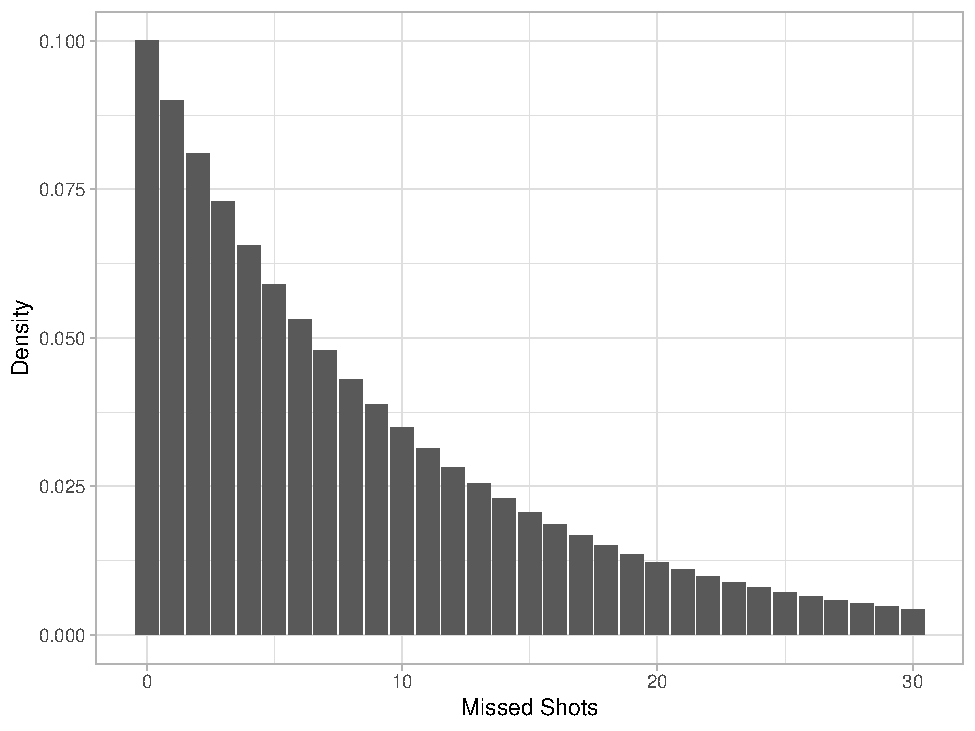
\includegraphics[width=0.8\linewidth]{famousdistrib_files/figure-latex/geom-plot-1} 

}

\caption{Histogram of basketball player's shot probabilities}\label{fig:geom-plot}
\end{figure}

Each ith value on the x axis and its corresponding jth y value can be conceptualized as ``There is a j probability that the basketball player had i failures before his first successful free throw.''

As suggested in the plot above, the probability that a shot is the first success approaches 0 as the observation number approaches infinity.

Now let's talk about the \texttt{stat} argument in \texttt{geom\_bar}. By default, this is set to \texttt{"count"}. This means that the height of an x-value's bar is determined by the number of times that it appears in a dataset. By changing this argument to \texttt{"identity}", ggplot looks for a corresponding y aesthetic to determine the height of the bar.

If we don't alter the behavior of \texttt{geom\_bar} we would get a plot that looks like this:

\begin{Shaded}
\begin{Highlighting}[]
\CommentTok{\# Don\textquotesingle{}t do this!}
\FunctionTok{ggplot}\NormalTok{(dgeom\_df) }\SpecialCharTok{+}
  \FunctionTok{geom\_bar}\NormalTok{(}\FunctionTok{aes}\NormalTok{(}\AttributeTok{x =}\NormalTok{ failures)) }\SpecialCharTok{+}
  \FunctionTok{labs}\NormalTok{(}\AttributeTok{x =} \StringTok{"Missed Shots"}\NormalTok{, }\AttributeTok{y =} \StringTok{"Density"}\NormalTok{)}
\end{Highlighting}
\end{Shaded}

\textbackslash begin\{figure\}

\{\centering 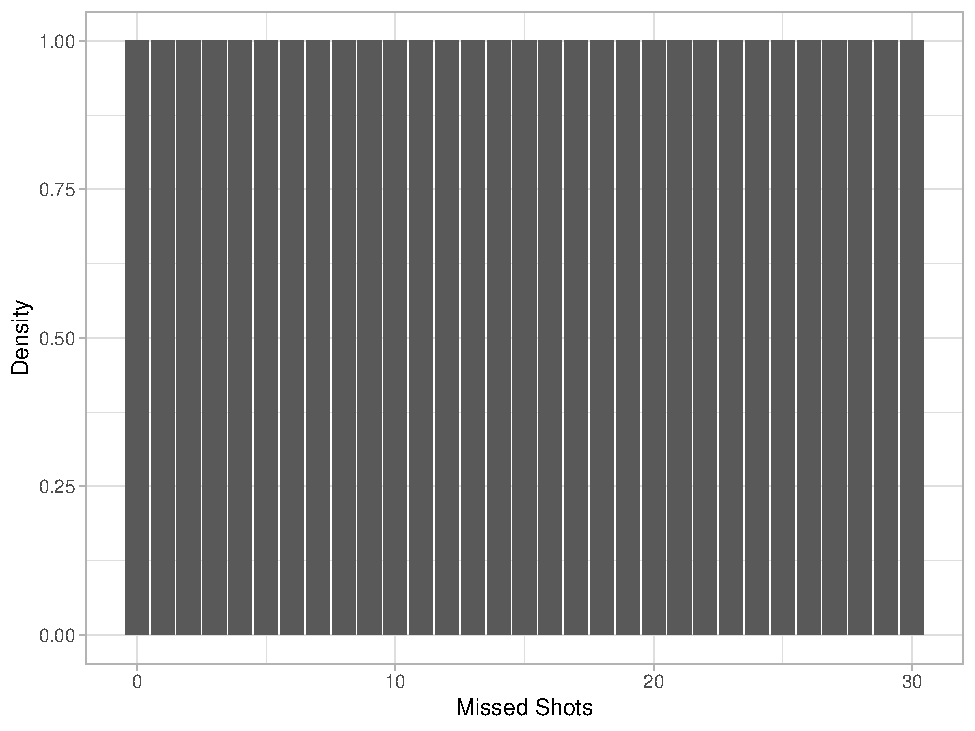
\includegraphics[width=0.8\linewidth]{famousdistrib_files/figure-latex/geomplot-incorrect-1}

\}

\textbackslash caption\{Incorrect geom\_bar plot\}\label{fig:geomplot-incorrect}
\textbackslash end\{figure\}

\begin{center}\rule{0.5\linewidth}{0.5pt}\end{center}

To calculate the probability of a range of outcomes we can use the function \texttt{pgeom}. For example, how likely is it that the player can make a free throw in 9 or fewer shots? To find this, we'll plug in \(q = 8\).

\begin{Shaded}
\begin{Highlighting}[]
\CommentTok{\# Create a cumulative density function}
\FunctionTok{pgeom}\NormalTok{(}\DecValTok{8}\NormalTok{, }\FloatTok{0.1}\NormalTok{)}
\end{Highlighting}
\end{Shaded}

\begin{verbatim}
## [1] 0.6125795
\end{verbatim}

We plug in \(q=8\) instead of \(q=9\) because the first argument of function requires the number of failures until the first success. In other words, the value that \texttt{pgeom} returns can be thought of as the probability that we have less than or equal to 8 failures before the first successful free throw.

When using a ``p'' or distribution function with \texttt{lower.tail\ =\ TRUE}, the first argument is our right bound. If we change to \texttt{lower.tail\ =\ FALSE}, the first argument becomes our left bound.

We can think of our calculation above as the same as finding the area of the binomial distribution from 0 to 8--i.e.~the total area of the first nine rectangles. We will fill the first nine bars blue and the rest gray.

\begin{Shaded}
\begin{Highlighting}[]
\FunctionTok{ggplot}\NormalTok{(dgeom\_df) }\SpecialCharTok{+} \CommentTok{\# Insert the vector of densities into the data argument}
  \FunctionTok{geom\_bar}\NormalTok{(}\FunctionTok{aes}\NormalTok{(}\AttributeTok{x =}\NormalTok{ failures, }\AttributeTok{y =}\NormalTok{ density),}
           \AttributeTok{stat =} \StringTok{"identity"}\NormalTok{,}
           \AttributeTok{fill =} \FunctionTok{ifelse}\NormalTok{(dgeom\_df}\SpecialCharTok{$}\NormalTok{failures }\SpecialCharTok{\textless{}=} \DecValTok{8}\NormalTok{, }\StringTok{"skyblue1"}\NormalTok{, }\StringTok{"grey35"}\NormalTok{)) }\SpecialCharTok{+}
  \FunctionTok{labs}\NormalTok{(}\AttributeTok{x =} \StringTok{"Missed Shots"}\NormalTok{, }\AttributeTok{y =} \StringTok{"Density"}\NormalTok{)}
\end{Highlighting}
\end{Shaded}

\begin{figure}

{\centering 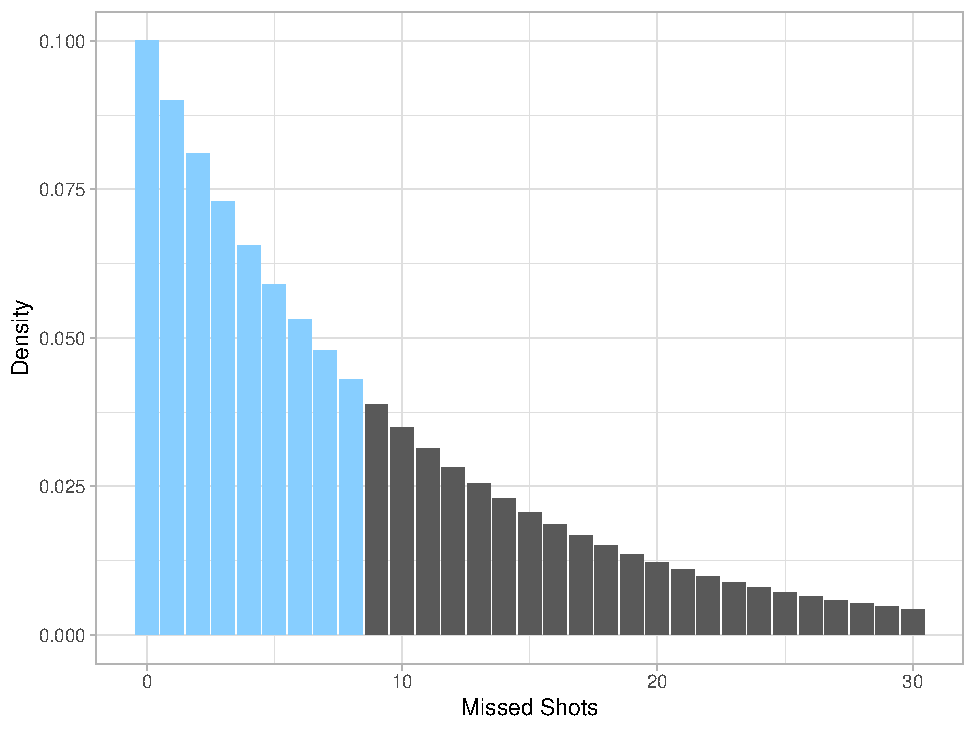
\includegraphics[width=0.8\linewidth]{famousdistrib_files/figure-latex/pgeom-plot-1} 

}

\caption{Basketball plot highlighting area of first 9 failures}\label{fig:pgeom-plot}
\end{figure}

Here are a few things to remember from the code above before we move on.

-The \texttt{ifelse} function is in base R and allows us to set a condition for the fill aesthetic of our bar plot. We are essentially telling ggplot to fill each bar blue if the \texttt{shot\_num} is less than or equal to 9. Otherwise, fill the rest of the bars gray.

-By default, the \texttt{lower.tail} argument is set to \texttt{TRUE}, meaning that we are finding the area of the distribution from the first shot to the ninth shot. However, if we set the \texttt{lower.tail} argument to \texttt{FALSE}, we will get the area of the distribution after the eighth shot.

\begin{Shaded}
\begin{Highlighting}[]
\FunctionTok{pgeom}\NormalTok{(}\DecValTok{8}\NormalTok{, }\AttributeTok{prob =} \FloatTok{0.1}\NormalTok{, }\AttributeTok{lower.tail =} \ConstantTok{FALSE}\NormalTok{)}
\end{Highlighting}
\end{Shaded}

\begin{verbatim}
## [1] 0.3874205
\end{verbatim}

\begin{Shaded}
\begin{Highlighting}[]
\CommentTok{\# As represented on a bar plot}
\FunctionTok{ggplot}\NormalTok{(dgeom\_df) }\SpecialCharTok{+}
  \FunctionTok{geom\_bar}\NormalTok{(}\FunctionTok{aes}\NormalTok{(}\AttributeTok{x =}\NormalTok{ failures, }\AttributeTok{y =}\NormalTok{ density),}
           \AttributeTok{stat =} \StringTok{"identity"}\NormalTok{,}
           \AttributeTok{fill =} \FunctionTok{ifelse}\NormalTok{(dgeom\_df}\SpecialCharTok{$}\NormalTok{failures }\SpecialCharTok{\textgreater{}} \DecValTok{8}\NormalTok{, }\StringTok{"skyblue1"}\NormalTok{, }\StringTok{"grey35"}\NormalTok{)) }\SpecialCharTok{+}
  \FunctionTok{labs}\NormalTok{(}\AttributeTok{x =} \StringTok{"Missed Shots"}\NormalTok{, }\AttributeTok{y =} \StringTok{"Density"}\NormalTok{)}
\end{Highlighting}
\end{Shaded}

\begin{figure}

{\centering 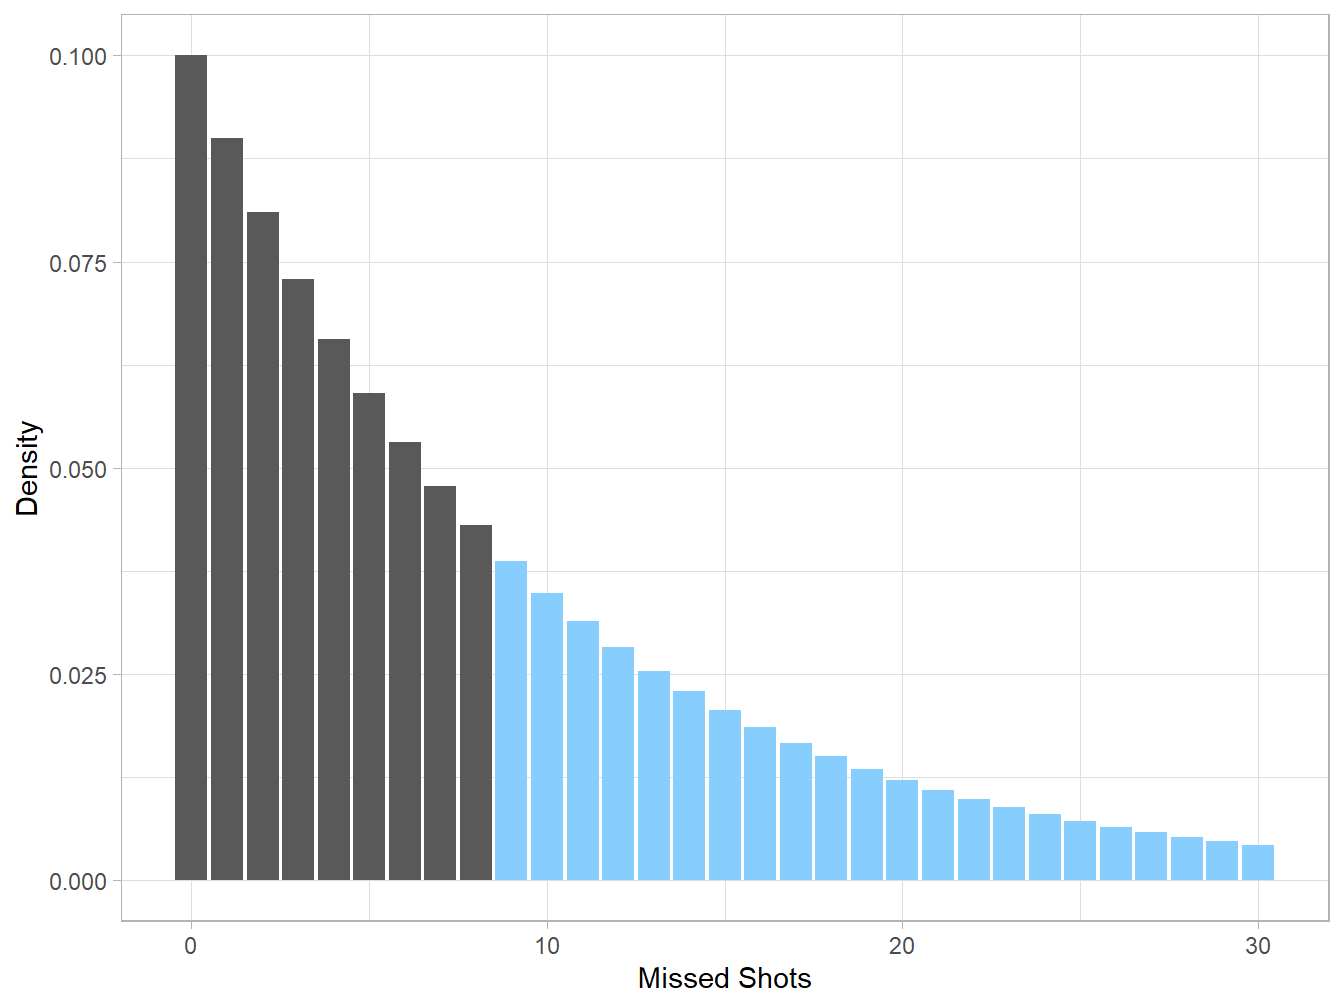
\includegraphics[width=0.8\linewidth]{famousdistrib_files/figure-latex/pgeomupper-plot-1} 

}

\caption{Basketball plot highlighting area after 8th failed shot}\label{fig:pgeomupper-plot}
\end{figure}

\begin{center}\rule{0.5\linewidth}{0.5pt}\end{center}

The \texttt{qgeom} function can be thought of as the inverse of \texttt{pgeom}. Because of this, we enter in a cumulative density (value from 0-1) into the function and it returns the shot number in which we would expect to reach that cumulative density, from left to right on a number line.

Like \texttt{pgeom}, keep in mind that \texttt{lower.tail} is set to \texttt{TRUE} by default.

By what shot can we begin expecting the player have already made a free throw? To answer this question, we will enter 50\% as a cumulative density.

\begin{Shaded}
\begin{Highlighting}[]
\FunctionTok{qgeom}\NormalTok{(}\FloatTok{0.5}\NormalTok{, }\AttributeTok{prob =} \FloatTok{0.1}\NormalTok{)}
\end{Highlighting}
\end{Shaded}

\begin{verbatim}
## [1] 6
\end{verbatim}

\begin{Shaded}
\begin{Highlighting}[]
\NormalTok{dgeom\_df }\OtherTok{\textless{}{-}}\NormalTok{ dgeom\_df }\SpecialCharTok{\%\textgreater{}\%}
  \FunctionTok{mutate}\NormalTok{(}\AttributeTok{cume\_dist =} \FunctionTok{cumsum}\NormalTok{(density))}

\FunctionTok{ggplot}\NormalTok{(dgeom\_df) }\SpecialCharTok{+}
  \FunctionTok{geom\_bar}\NormalTok{(}\FunctionTok{aes}\NormalTok{(}\AttributeTok{x =}\NormalTok{ failures, }\AttributeTok{y =}\NormalTok{ density),}
           \AttributeTok{stat =} \StringTok{"identity"}\NormalTok{,}
           \AttributeTok{fill =} \FunctionTok{ifelse}\NormalTok{(dgeom\_df}\SpecialCharTok{$}\NormalTok{cume\_dist }\SpecialCharTok{\textless{}=}\NormalTok{.}\DecValTok{5}\NormalTok{, }\StringTok{"skyblue1"}\NormalTok{, }\StringTok{"grey35"}\NormalTok{)) }\SpecialCharTok{+}
  \FunctionTok{labs}\NormalTok{(}\AttributeTok{x =} \StringTok{"Missed Shots"}\NormalTok{, }\AttributeTok{y =} \StringTok{"Density"}\NormalTok{)}
\end{Highlighting}
\end{Shaded}

\textbackslash begin\{figure\}

\{\centering 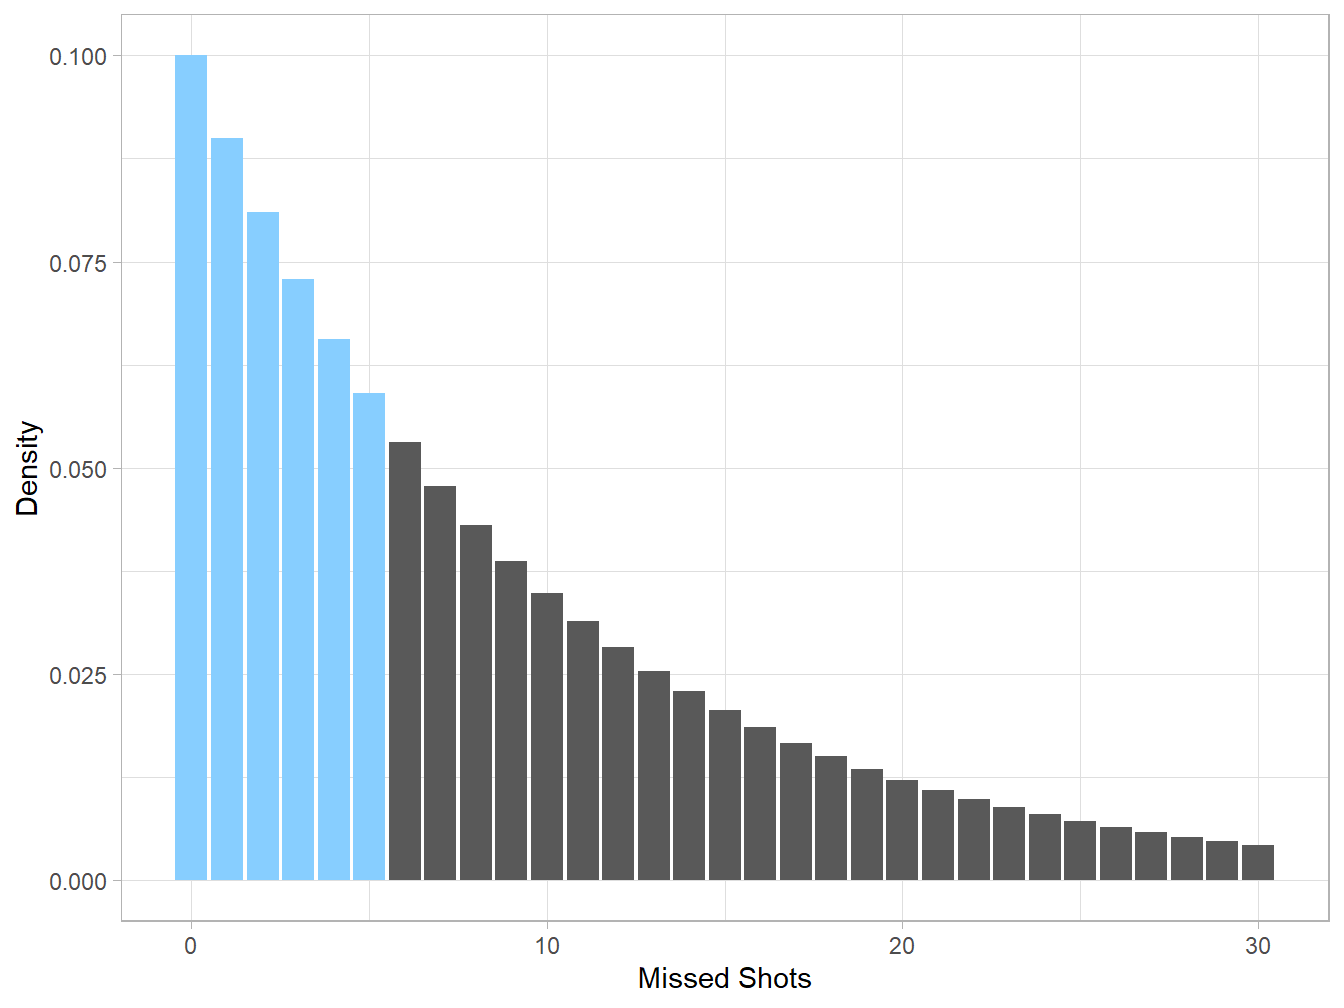
\includegraphics[width=0.8\linewidth]{famousdistrib_files/figure-latex/qgeom-plot-1}

\}

\textbackslash caption\{Basketball plot highlighting lower 50\% of distribution\}\label{fig:qgeom-plot}
\textbackslash end\{figure\}

There is quite a bit to unpack here. We use \texttt{mutate} to create a new variable for the cumulative density at each shot. This is the sum of a shot's density and all of the previous shots before it.

Next, we return to the \texttt{ifelse} function to determine which bars to fill. We can interpret our code as ``If the cumulative density of this shot is less than or equal to .5, fill it blue; otherwise, fill it gray.''

\begin{center}\rule{0.5\linewidth}{0.5pt}\end{center}

Finally, imagine that 1,000 exact copies of the basketball player shoot free throws. Below is the distribution of those outcomes. The function \texttt{rgeom} simulates each of the 1,000 players and returns the number of their first successful shot.

\begin{Shaded}
\begin{Highlighting}[]
\NormalTok{rand\_geom }\OtherTok{\textless{}{-}} \FunctionTok{tibble}\NormalTok{(}\AttributeTok{deviates =} \FunctionTok{rgeom}\NormalTok{(}\DecValTok{1000}\NormalTok{, }\FloatTok{0.1}\NormalTok{))}

\FunctionTok{ggplot}\NormalTok{(rand\_geom) }\SpecialCharTok{+}
  \FunctionTok{geom\_histogram}\NormalTok{(}\FunctionTok{aes}\NormalTok{(}\AttributeTok{x =}\NormalTok{ deviates),}
                 \AttributeTok{binwidth =} \DecValTok{2}\NormalTok{) }\SpecialCharTok{+}
  \FunctionTok{labs}\NormalTok{(}\AttributeTok{x =} \StringTok{"First Shot"}\NormalTok{, }\AttributeTok{y =} \StringTok{"Frequency"}\NormalTok{) }\SpecialCharTok{+}
  \FunctionTok{scale\_x\_continuous}\NormalTok{(}\AttributeTok{breaks =} \FunctionTok{seq}\NormalTok{(}\DecValTok{0}\NormalTok{, }\DecValTok{80}\NormalTok{, }\DecValTok{10}\NormalTok{)) }\CommentTok{\# Added more ticks on x axis}
\end{Highlighting}
\end{Shaded}

\begin{figure}

{\centering 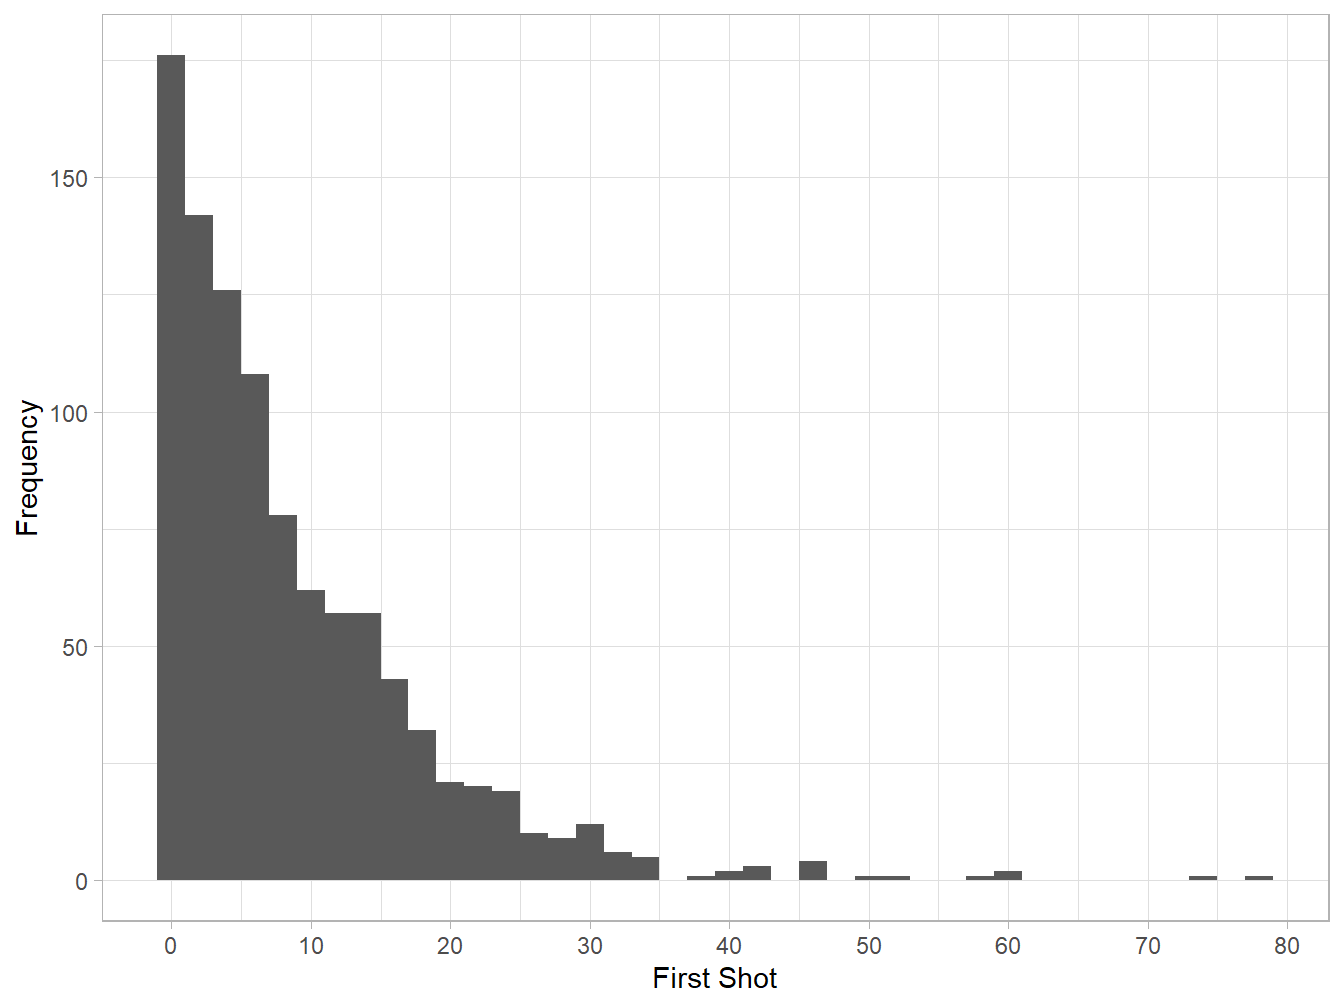
\includegraphics[width=0.8\linewidth]{famousdistrib_files/figure-latex/rgeom-plot-1} 

}

\caption{Plot of 1,000 random geometric deviates}\label{fig:rgeom-plot}
\end{figure}

As stated at the beginning of this chapter, the geometric distribution can be thought of the spread of N trials required to get probability p.~Because of this, as we increase the number of simulated basketball players, we reach a distribution more and more similar to the actual binomial distribution.

To visualize this, we'll generate four plots: three randomly-sampled geometric distributions and a ``true'' geometric distribution. To simplify our code, we'll start by writing a new function called \texttt{geom\_plot}. If function-writing is unfamiliar to you, I encourage you to read this \href{https://r4ds.had.co.nz/functions.html}{friendly introduction}.

\begin{Shaded}
\begin{Highlighting}[]
\CommentTok{\# Create a function that randomly samples from geometric distribution with sample size n}
\NormalTok{geom\_plot }\OtherTok{\textless{}{-}} \ControlFlowTok{function}\NormalTok{(prob, n)\{}
\NormalTok{  temp }\OtherTok{\textless{}{-}} \FunctionTok{tibble}\NormalTok{(}\AttributeTok{deviates =} \FunctionTok{rgeom}\NormalTok{(n, prob))}
\NormalTok{  plot }\OtherTok{\textless{}{-}} \FunctionTok{ggplot}\NormalTok{(temp, }\FunctionTok{aes}\NormalTok{(}\AttributeTok{x =}\NormalTok{ deviates)) }\SpecialCharTok{+} 
    \FunctionTok{geom\_histogram}\NormalTok{(}\AttributeTok{binwidth =} \DecValTok{2}\NormalTok{) }\SpecialCharTok{+}
    \FunctionTok{scale\_x\_continuous}\NormalTok{(}\AttributeTok{breaks =} \FunctionTok{seq}\NormalTok{(}\DecValTok{0}\NormalTok{, }\DecValTok{80}\NormalTok{, }\DecValTok{20}\NormalTok{)) }\SpecialCharTok{+}
    \FunctionTok{labs}\NormalTok{(}\AttributeTok{x =} \ConstantTok{NULL}\NormalTok{, }\AttributeTok{y =} \ConstantTok{NULL}\NormalTok{, }\AttributeTok{caption =} \FunctionTok{str\_c}\NormalTok{(n, }\StringTok{"simulations"}\NormalTok{, }\AttributeTok{sep =} \StringTok{" "}\NormalTok{))}
  \FunctionTok{return}\NormalTok{(plot)}
\NormalTok{\}}
 
\CommentTok{\# Generate random samples and plots}
\NormalTok{sample\_1000 }\OtherTok{\textless{}{-}} \FunctionTok{geom\_plot}\NormalTok{(}\FloatTok{0.1}\NormalTok{, }\DecValTok{1000}\NormalTok{) }\SpecialCharTok{+}
  \FunctionTok{labs}\NormalTok{(}\AttributeTok{y =} \StringTok{"Count"}\NormalTok{,}
       \AttributeTok{title =} \StringTok{"Random Deviates"}\NormalTok{)}
\NormalTok{sample\_10000 }\OtherTok{\textless{}{-}} \FunctionTok{geom\_plot}\NormalTok{(}\FloatTok{0.1}\NormalTok{, }\DecValTok{10000}\NormalTok{)}
\NormalTok{sample\_100000 }\OtherTok{\textless{}{-}} \FunctionTok{geom\_plot}\NormalTok{(}\FloatTok{0.1}\NormalTok{, }\DecValTok{100000}\NormalTok{)}


\CommentTok{\# Generate true geometric distribution }
\NormalTok{dgeom }\OtherTok{\textless{}{-}} \FunctionTok{tibble}\NormalTok{(}\AttributeTok{shot\_num =} \DecValTok{1}\SpecialCharTok{:}\DecValTok{80}\NormalTok{,}
                \AttributeTok{density =} \FunctionTok{dgeom}\NormalTok{(}\DecValTok{1}\SpecialCharTok{:}\DecValTok{80}\NormalTok{, }\AttributeTok{prob =} \FloatTok{0.1}\NormalTok{, }\AttributeTok{log =} \ConstantTok{FALSE}\NormalTok{))}

\NormalTok{true\_plot }\OtherTok{\textless{}{-}} \FunctionTok{ggplot}\NormalTok{(dgeom) }\SpecialCharTok{+}
  \FunctionTok{geom\_bar}\NormalTok{(}\FunctionTok{aes}\NormalTok{(}\AttributeTok{x =}\NormalTok{ shot\_num, }\AttributeTok{y =}\NormalTok{ density), }\AttributeTok{stat =} \StringTok{"identity"}\NormalTok{, }\AttributeTok{width =} \FloatTok{0.5}\NormalTok{) }\SpecialCharTok{+}
  \FunctionTok{labs}\NormalTok{(}\AttributeTok{x =} \StringTok{"First Shot"}\NormalTok{, }
       \AttributeTok{y =} \StringTok{"Density"}\NormalTok{, }
       \AttributeTok{title =} \StringTok{"Geometric Distribution"}\NormalTok{) }\SpecialCharTok{+}
  \FunctionTok{scale\_x\_continuous}\NormalTok{(}\AttributeTok{breaks =} \FunctionTok{seq}\NormalTok{(}\DecValTok{0}\NormalTok{, }\DecValTok{80}\NormalTok{, }\DecValTok{20}\NormalTok{))}

\CommentTok{\# Plot all together in a grid}
\NormalTok{cowplot}\SpecialCharTok{::}\FunctionTok{plot\_grid}\NormalTok{(}\ConstantTok{NULL}\NormalTok{, true\_plot, }\ConstantTok{NULL}\NormalTok{, sample\_1000, sample\_10000, sample\_100000, }\AttributeTok{ncol =} \DecValTok{3}\NormalTok{, }\AttributeTok{nrow =} \DecValTok{2}\NormalTok{)}
\end{Highlighting}
\end{Shaded}

\begin{center}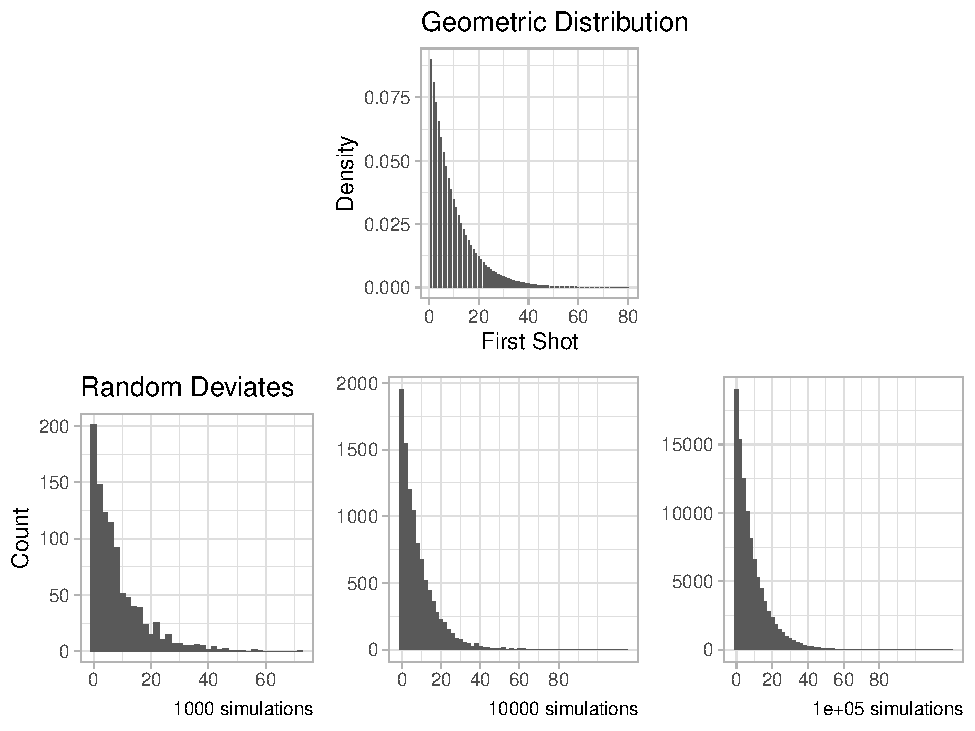
\includegraphics[width=0.8\linewidth]{famousdistrib_files/figure-latex/sample-plot-1} \end{center}

\hypertarget{Binomial}{%
\subsection{Binomial Distribution}\label{Binomial}}

While we would use the geometric distribution to model the number of failed free throws until a successful shot, the \textbf{binomial distribution} instead considers the probability of successful free throws in a fixed number of attempts. It is defined below:

\[P(K = k) = C_{n,k}p^{k}(1-p)^{n-k}\\\textrm{where} \hspace{0.2cm}C_{n,k}\hspace{0.2cm}\textrm{is the number of ways that we can pick k successes in n trials.}\]

At first glance, this formula is complicated, but it can be easily divided into two parts:

\begin{itemize}
\item
  \(C_{k,n}\) represents the number of ways we can select k successes in n trials. This combination can be calculated as \(C_{n,k}=\frac{n!}{k!(n-k)!}\).
\item
  \(p^{k}(1-p)^{n-k}\) or the probability of getting k successes and therefore n-k failures.
\end{itemize}

We multiply the scenarios term by the probability term to account for the fact that there are multiple ways that we can get to the kth success. A basketball player does not need to make k shots in a particular order.

For example, if we are interested in the probability that the basketball player shoots 30 free throws and makes 3 of them, we can plug these numbers into our equation.

\begin{itemize}
\item
  We have n = 30 independent trials, assuming that the player shoots at the same place and does not get tired.
\item
  We want to have k = 3 successful free throws and n- k = 27 unsuccessful ones.
\item
  Recall that the probability of a successful shot is p = 10\%. Thus, a missed shot has probability 1 - p = 90\%.
\end{itemize}

Thus, our density formula allows us to find the probability of a basketball player making 3 shots using simple multiplication.

\[P(K = 3) = C_{30,3}(.10)^{3}(1-.10)^{27}\approx.2361\]

With R, the function \texttt{dbinom} similarly accomplishes this.

\begin{Shaded}
\begin{Highlighting}[]
\CommentTok{\# The arguments do not all need to be named, but I will do so here.}
\FunctionTok{dbinom}\NormalTok{(}\AttributeTok{x =} \DecValTok{3}\NormalTok{, }\AttributeTok{size =} \DecValTok{30}\NormalTok{, }\AttributeTok{prob =}\NormalTok{ .}\DecValTok{1}\NormalTok{)}
\end{Highlighting}
\end{Shaded}

\begin{verbatim}
## [1] 0.2360879
\end{verbatim}

In other words, the probability that the basketball player shoots 30 free throws and makes \textbf{exactly} 3 of them is about 0.2361.

As we begin visualizing this with \texttt{ggplot}, we should return to our strategy from the geometric chapter by creating a data frame or tibble with two columns--one to signify all of the possible number of successes that we can have, and another of their corresponding probabilities or densities.

\begin{Shaded}
\begin{Highlighting}[]
\NormalTok{dbinom\_df }\OtherTok{\textless{}{-}} \FunctionTok{tibble}\NormalTok{(}\AttributeTok{shots =} \DecValTok{0}\SpecialCharTok{:}\DecValTok{30}\NormalTok{,}
                 \AttributeTok{density =} \FunctionTok{dbinom}\NormalTok{(}\DecValTok{0}\SpecialCharTok{:}\DecValTok{30}\NormalTok{, }\AttributeTok{size =} \DecValTok{30}\NormalTok{, }\AttributeTok{prob =}\NormalTok{ .}\DecValTok{1}\NormalTok{))}
\end{Highlighting}
\end{Shaded}

We can now plot this with \texttt{geom\_bar}.

\begin{Shaded}
\begin{Highlighting}[]
\FunctionTok{ggplot}\NormalTok{(dbinom\_df) }\SpecialCharTok{+}
  \FunctionTok{geom\_bar}\NormalTok{(}\FunctionTok{aes}\NormalTok{(}\AttributeTok{x =}\NormalTok{ shots, }\AttributeTok{y =}\NormalTok{ density),}
           \AttributeTok{stat =} \StringTok{"identity"}\NormalTok{) }\SpecialCharTok{+}
  \FunctionTok{labs}\NormalTok{(}\AttributeTok{x =} \StringTok{"Successful Shots"}\NormalTok{, }\AttributeTok{y =} \StringTok{"Density"}\NormalTok{) }\SpecialCharTok{+}
  \FunctionTok{scale\_x\_continuous}\NormalTok{(}\AttributeTok{breaks =} \FunctionTok{seq}\NormalTok{(}\DecValTok{0}\NormalTok{, }\DecValTok{30}\NormalTok{, }\DecValTok{2}\NormalTok{))}
\end{Highlighting}
\end{Shaded}

\begin{center}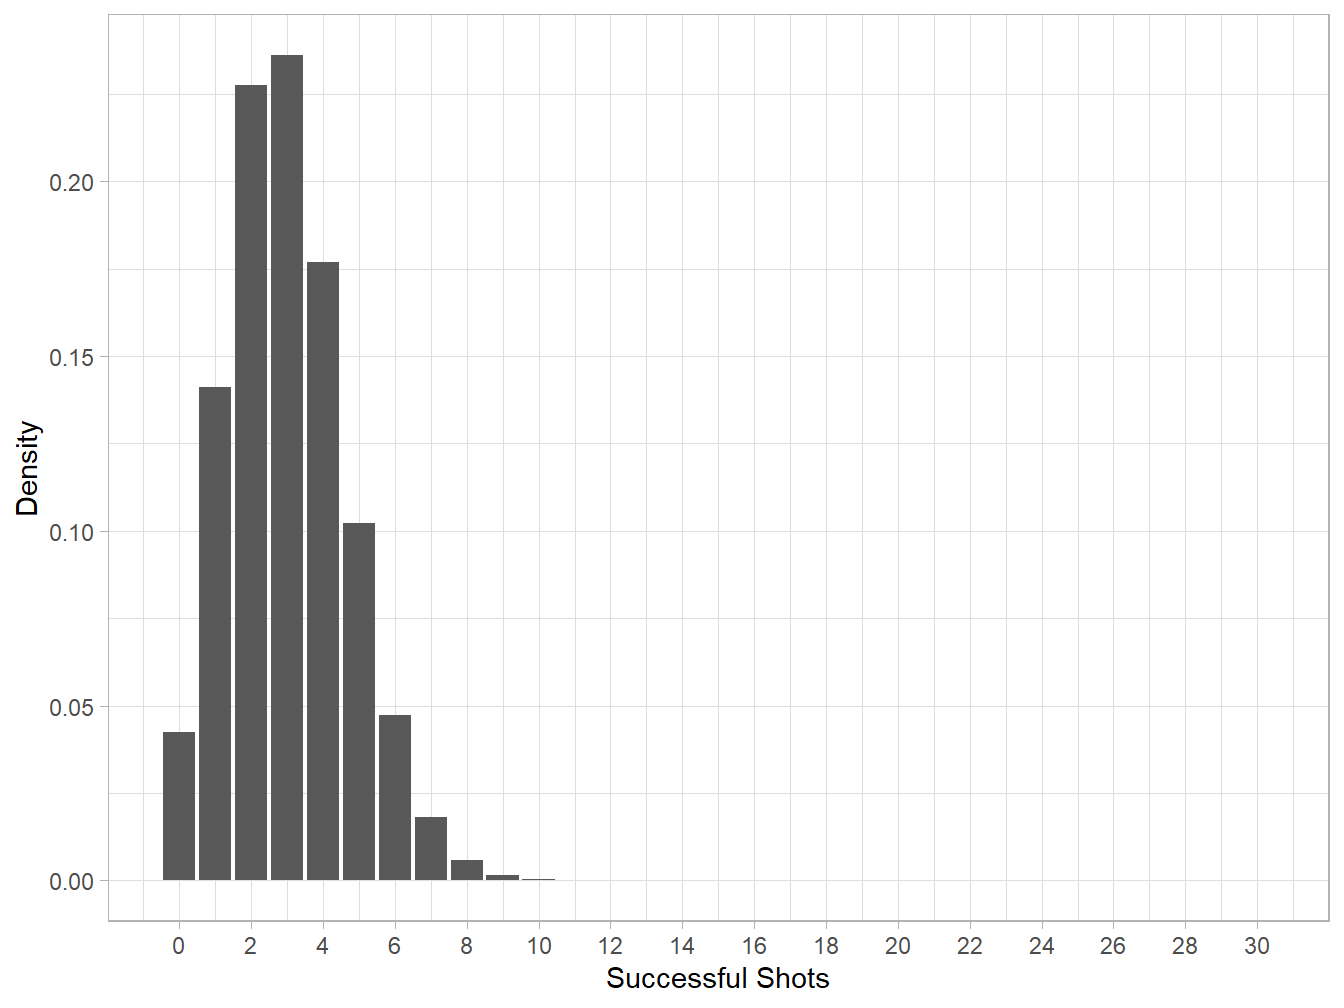
\includegraphics[width=0.8\linewidth]{famousdistrib_files/figure-latex/binom-plot-1} \end{center}

As seen above, it is quite unlikely that the basketball player will make more than 10 shots. In fact, their probabilities aren't even large enough for the bars to register on the plot.

\begin{center}\rule{0.5\linewidth}{0.5pt}\end{center}

In some scenarios in the statistics world, we aren't only interested in the probability of getting \textbf{exactly} k successes; we may want to consider a range of outcomes. For example, a personal coach who records the basketball player's progress wants to determine the probability that he makes 3 \textbf{or fewer} shots out of 30.

Using the previous chapters, we can assume that we would want to use the distribution function \texttt{pbinom} to answer this question.

\begin{Shaded}
\begin{Highlighting}[]
\CommentTok{\# Before you continue, think about what the four arguments mean. Why would we set the lower.tail to TRUE instead of FALSE?}
\FunctionTok{pbinom}\NormalTok{(}\DecValTok{3}\NormalTok{, }\DecValTok{30}\NormalTok{, }\FloatTok{0.1}\NormalTok{, }\AttributeTok{lower.tail =} \ConstantTok{TRUE}\NormalTok{)}
\end{Highlighting}
\end{Shaded}

\begin{verbatim}
## [1] 0.6474392
\end{verbatim}

The first argument in the above function is similar to the other ``p'' functions since it can be thought of as the ``right bound'' of interest. We can imagine the \texttt{pbinom} function as finding the area of the binomial distribution from 0 to 3.

\begin{Shaded}
\begin{Highlighting}[]
\FunctionTok{ggplot}\NormalTok{(dbinom\_df) }\SpecialCharTok{+}
  \FunctionTok{geom\_bar}\NormalTok{(}\FunctionTok{aes}\NormalTok{(}\AttributeTok{x =}\NormalTok{ shots, }\AttributeTok{y =}\NormalTok{ density),}
           \AttributeTok{stat =} \StringTok{"identity"}\NormalTok{,}
           \AttributeTok{fill =} \FunctionTok{ifelse}\NormalTok{(dbinom\_df}\SpecialCharTok{$}\NormalTok{shots }\SpecialCharTok{\textless{}=} \DecValTok{3}\NormalTok{, }\StringTok{"purple2"}\NormalTok{, }\StringTok{"lightgray"}\NormalTok{)) }\SpecialCharTok{+}
  \FunctionTok{labs}\NormalTok{(}\AttributeTok{x =} \StringTok{"Successful Shots"}\NormalTok{, }\AttributeTok{y =} \StringTok{"Density"}\NormalTok{)}
\end{Highlighting}
\end{Shaded}

\begin{center}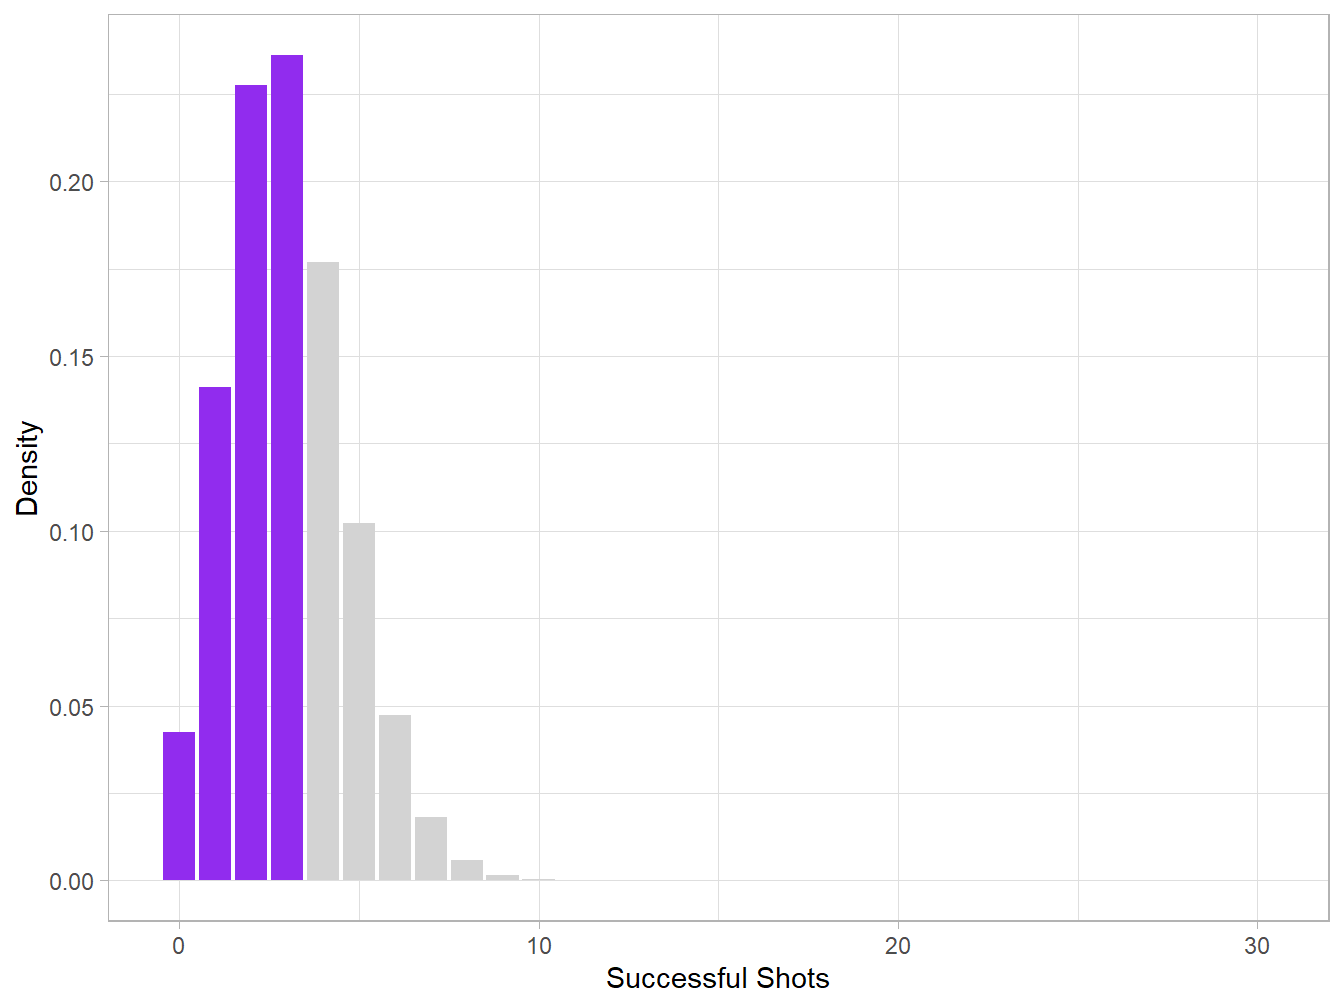
\includegraphics[width=0.8\linewidth]{famousdistrib_files/figure-latex/pbinom-plot-1} \end{center}

Just as we used it in the geometric distribution section, the \texttt{ifelse} function allows us to fill our bars with different colors depending on the ``shot'' value. The interpretation here is ``fill the bar purple if number of successful shots is three or fewer. If not, fill the bar gray.''

\begin{center}\rule{0.5\linewidth}{0.5pt}\end{center}

Like the other ``r'' functions,\texttt{rbinom} randomly simulates the outcomes of a distribution. In this case, the function returns the number of successful free throws made all of the simulations. This is useful because it helps us better understand the natural random process.

\begin{Shaded}
\begin{Highlighting}[]
\NormalTok{ranbinom }\OtherTok{\textless{}{-}} \FunctionTok{tibble}\NormalTok{(}\AttributeTok{deviates =} \FunctionTok{rbinom}\NormalTok{(}\DecValTok{1000}\NormalTok{, }\DecValTok{30}\NormalTok{, .}\DecValTok{10}\NormalTok{))}

\FunctionTok{glimpse}\NormalTok{(ranbinom)}
\end{Highlighting}
\end{Shaded}

\begin{verbatim}
## Rows: 1,000
## Columns: 1
## $ deviates <int> 2, 1, 2, 6, 0, 2, 3, 6, 4, 1, 3, 4, 8, 1, 3, 0, 5, 3, 3, 3, 4~
\end{verbatim}

\begin{Shaded}
\begin{Highlighting}[]
\FunctionTok{ggplot}\NormalTok{(ranbinom) }\SpecialCharTok{+}
  \FunctionTok{geom\_bar}\NormalTok{(}\FunctionTok{aes}\NormalTok{(}\AttributeTok{x =}\NormalTok{ deviates), }\AttributeTok{stat =} \StringTok{"count"}\NormalTok{) }\SpecialCharTok{+}
  \FunctionTok{scale\_x\_continuous}\NormalTok{(}\AttributeTok{breaks =} \FunctionTok{seq}\NormalTok{(}\DecValTok{0}\NormalTok{,}\DecValTok{10}\NormalTok{, }\DecValTok{1}\NormalTok{)) }\SpecialCharTok{+}
  \FunctionTok{labs}\NormalTok{(}\AttributeTok{x =} \StringTok{"Successful Shots"}\NormalTok{, }\AttributeTok{y =} \StringTok{"Frequency"}\NormalTok{)}
\end{Highlighting}
\end{Shaded}

\begin{center}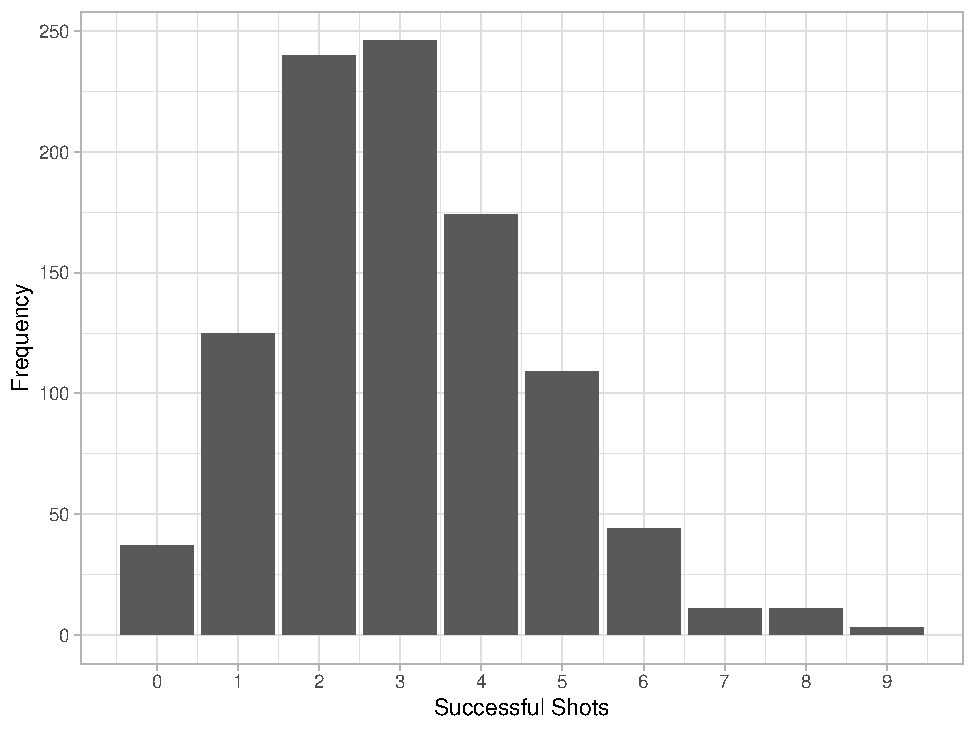
\includegraphics[width=0.8\linewidth]{famousdistrib_files/figure-latex/rbinom-1} \end{center}

\begin{center}\rule{0.5\linewidth}{0.5pt}\end{center}

\hypertarget{negative-binomial-distribution}{%
\subsection{Negative Binomial Distribution}\label{negative-binomial-distribution}}

Next, we'll introduce the \textbf{negative binomial distribution}. Similar to the from the geometric distribution, we are interested in modeling the number of failures in a binary process. However, we are not only interested in how long it takes for one success; we are interested in modeling the number of failures until a particular number (\(r\)) of successes.

\[\begin{equation}
P(Y=y) = \binom{y + r - 1}{r-1} (1-p)^{y}(p)^r \quad \textrm{for}\quad y = 0, 1, \ldots, \infty.
\end{equation}\]

An interesting case appears when we set \(r=1\), i.e.~the number of failures until one success.

\[\begin{split}
P(Y=1) &= \binom{y + 1 - 1}{1-1} (1-p)^{y} (p)^1 \\ &= \binom{y}{0} (1-p)^yp \\ &=(1-p)^yp \quad \textrm{for} \quad y = 0, 1, \ldots, \infty
\end{split}\]

Notice how the last line of this looks exactly like the \textbf{geometric distribution}? This is because the geometric distribution is a special case of the negative binomial distribution.

Now let's return to the basketball example. As we have established before, there is about a 4\% chance that our player makes 8 failures before his first successful shot. What is the probability that he makes 8 failures before his second successful shot?

\begin{Shaded}
\begin{Highlighting}[]
\FunctionTok{dnbinom}\NormalTok{(}\DecValTok{8}\NormalTok{, }\DecValTok{2}\NormalTok{, }\FloatTok{0.1}\NormalTok{)}
\end{Highlighting}
\end{Shaded}

\begin{verbatim}
## [1] 0.03874205
\end{verbatim}

\begin{Shaded}
\begin{Highlighting}[]
\NormalTok{dnbinom\_df }\OtherTok{\textless{}{-}} \FunctionTok{tibble}\NormalTok{(}\AttributeTok{failures =} \DecValTok{0}\SpecialCharTok{:}\DecValTok{30}\NormalTok{,}
                  \AttributeTok{density =} \FunctionTok{dnbinom}\NormalTok{(}\DecValTok{0}\SpecialCharTok{:}\DecValTok{30}\NormalTok{, }\DecValTok{2}\NormalTok{, }\FloatTok{0.1}\NormalTok{))}

\FunctionTok{ggplot}\NormalTok{(dnbinom\_df, }\FunctionTok{aes}\NormalTok{(}\AttributeTok{x =}\NormalTok{ failures, }\AttributeTok{y =}\NormalTok{ density)) }\SpecialCharTok{+}
  \FunctionTok{geom\_bar}\NormalTok{(}\AttributeTok{stat =} \StringTok{"identity"}\NormalTok{, }\AttributeTok{fill =} \StringTok{"turquoise1"}\NormalTok{, }\AttributeTok{color =} \StringTok{"black"}\NormalTok{) }\SpecialCharTok{+}
  \FunctionTok{labs}\NormalTok{(}\AttributeTok{x =} \StringTok{"Failed Shots"}\NormalTok{, }\AttributeTok{y =} \StringTok{"Density"}\NormalTok{, }
       \AttributeTok{title =} \StringTok{"Number of Failures until Second Free Throw"}\NormalTok{)}
\end{Highlighting}
\end{Shaded}

\begin{center}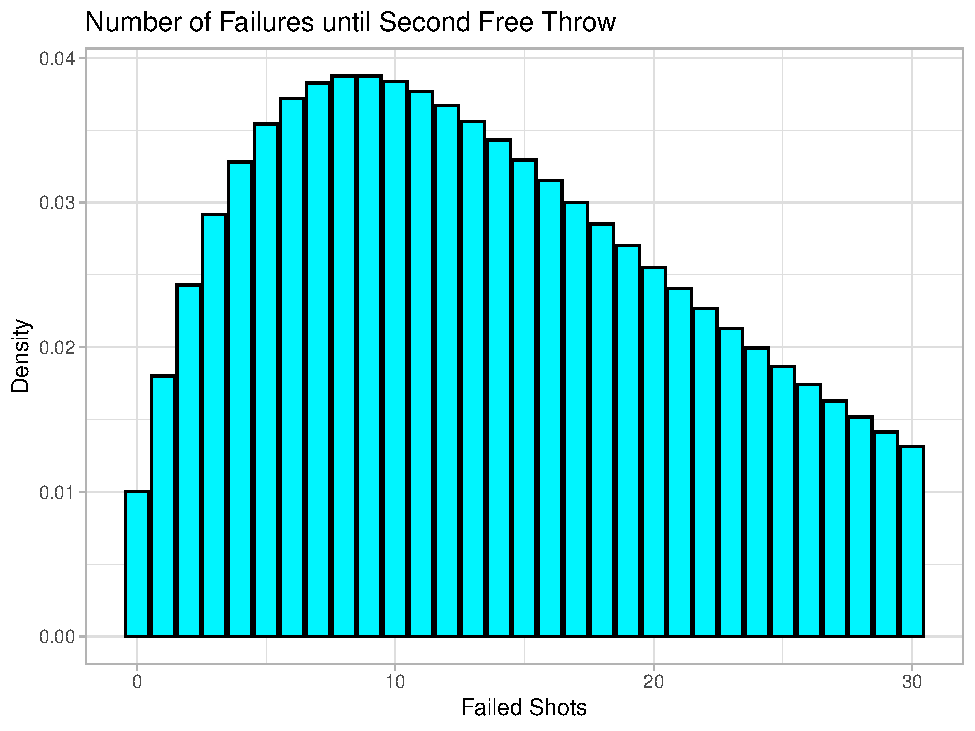
\includegraphics[width=0.8\linewidth]{famousdistrib_files/figure-latex/dnbinom-plot-1} \end{center}

Now that we have a new parameter r, how does the distribution change as it increases or decreases?

\begin{Shaded}
\begin{Highlighting}[]
\NormalTok{nbinom\_plot }\OtherTok{\textless{}{-}} \ControlFlowTok{function}\NormalTok{(x, size, prob)\{}
\NormalTok{  temp }\OtherTok{\textless{}{-}} \FunctionTok{tibble}\NormalTok{(}\AttributeTok{failures =}\NormalTok{ x,}
                 \AttributeTok{density =} \FunctionTok{dnbinom}\NormalTok{(x, size, prob),}
                 \AttributeTok{cume\_density =} \FunctionTok{cumsum}\NormalTok{(density))}
\NormalTok{  median }\OtherTok{\textless{}{-}}\NormalTok{ temp }\SpecialCharTok{\%\textgreater{}\%} \FunctionTok{filter}\NormalTok{(}\FunctionTok{between}\NormalTok{(cume\_density, .}\DecValTok{5}\NormalTok{, .}\DecValTok{55}\NormalTok{))}
\NormalTok{  plot }\OtherTok{\textless{}{-}} \FunctionTok{ggplot}\NormalTok{(temp, }\FunctionTok{aes}\NormalTok{(}\AttributeTok{x =}\NormalTok{ failures, }\AttributeTok{y =}\NormalTok{ density)) }\SpecialCharTok{+}
    \FunctionTok{geom\_density}\NormalTok{(}\AttributeTok{stat =} \StringTok{"identity"}\NormalTok{) }\SpecialCharTok{+}
    \FunctionTok{geom\_vline}\NormalTok{(}\AttributeTok{xintercept =}\NormalTok{ median}\SpecialCharTok{$}\NormalTok{failures[}\DecValTok{1}\NormalTok{]) }\SpecialCharTok{+}
    \FunctionTok{labs}\NormalTok{(}\AttributeTok{x =} \ConstantTok{NULL}\NormalTok{, }\AttributeTok{y =} \ConstantTok{NULL}\NormalTok{)}
  \FunctionTok{return}\NormalTok{(plot)}
\NormalTok{\}}

\NormalTok{p1 }\OtherTok{\textless{}{-}} \FunctionTok{nbinom\_plot}\NormalTok{(}\DecValTok{0}\SpecialCharTok{:}\DecValTok{100}\NormalTok{, }\DecValTok{3}\NormalTok{, }\FloatTok{0.1}\NormalTok{) }\SpecialCharTok{+}
  \FunctionTok{ggtitle}\NormalTok{(}\StringTok{"r = 3, prob = 0.1"}\NormalTok{)}
\NormalTok{p2 }\OtherTok{\textless{}{-}} \FunctionTok{nbinom\_plot}\NormalTok{(}\DecValTok{0}\SpecialCharTok{:}\DecValTok{100}\NormalTok{, }\DecValTok{5}\NormalTok{, }\FloatTok{0.1}\NormalTok{) }\SpecialCharTok{+}
  \FunctionTok{ggtitle}\NormalTok{(}\StringTok{"r = 5, prob = 0.1"}\NormalTok{) }\SpecialCharTok{+}
  \FunctionTok{labs}\NormalTok{(}\AttributeTok{x =} \StringTok{"Failures"}\NormalTok{, }\AttributeTok{y =} \StringTok{"Density"}\NormalTok{)}
\NormalTok{p3 }\OtherTok{\textless{}{-}} \FunctionTok{nbinom\_plot}\NormalTok{(}\DecValTok{0}\SpecialCharTok{:}\DecValTok{100}\NormalTok{, }\DecValTok{7}\NormalTok{, }\FloatTok{0.1}\NormalTok{) }\SpecialCharTok{+}
  \FunctionTok{ggtitle}\NormalTok{(}\StringTok{"r = 7, prob = 0.1"}\NormalTok{)}
\NormalTok{p4 }\OtherTok{\textless{}{-}} \FunctionTok{nbinom\_plot}\NormalTok{(}\DecValTok{0}\SpecialCharTok{:}\DecValTok{100}\NormalTok{, }\DecValTok{5}\NormalTok{, }\FloatTok{0.15}\NormalTok{) }\SpecialCharTok{+}
  \FunctionTok{ggtitle}\NormalTok{(}\StringTok{"r = 5, prob = 0.15"}\NormalTok{)}
\NormalTok{p5 }\OtherTok{\textless{}{-}} \FunctionTok{nbinom\_plot}\NormalTok{(}\DecValTok{0}\SpecialCharTok{:}\DecValTok{100}\NormalTok{, }\DecValTok{5}\NormalTok{, }\FloatTok{0.08}\NormalTok{) }\SpecialCharTok{+}
  \FunctionTok{ggtitle}\NormalTok{(}\StringTok{"r = 5, prob = 0.05"}\NormalTok{)}

\FunctionTok{plot\_grid}\NormalTok{(p1, }\ConstantTok{NULL}\NormalTok{, p4, }\ConstantTok{NULL}\NormalTok{, p2, }\ConstantTok{NULL}\NormalTok{, p3, }\ConstantTok{NULL}\NormalTok{, p5, }\AttributeTok{ncol =} \DecValTok{3}\NormalTok{, }\AttributeTok{nrow =} \DecValTok{3}\NormalTok{)}
\end{Highlighting}
\end{Shaded}

\begin{center}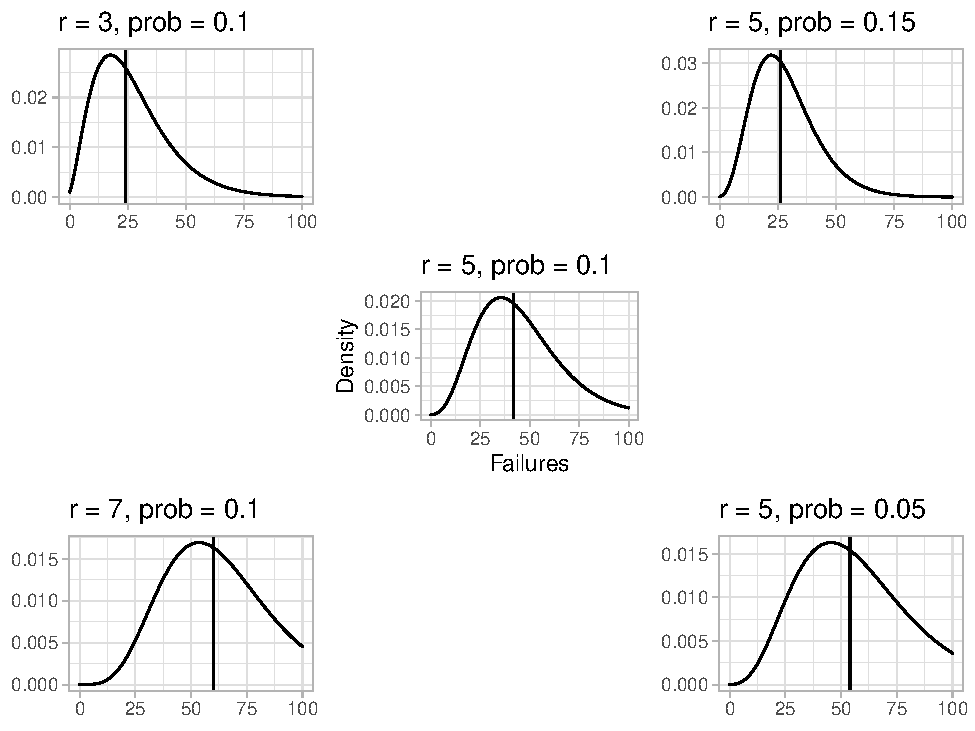
\includegraphics[width=0.8\linewidth]{famousdistrib_files/figure-latex/dnbinom-mult-1} \end{center}

As you can see above, the center of the distribution moves right as \(r\) increases or the probability of a success decreases.

\hypertarget{Poisson}{%
\subsection{Poisson Distribution}\label{Poisson}}

Unlike those based on Bernoulli processes (binary and independent outcomes), a \textbf{Poisson} process considers the number of times an event occurs in a given time or space. If \(K\), for instance, is the number of events in an interval, we'll model it with the \textbf{Poisson Distribution}.

\[
P(K=k) = \frac{e^{-\lambda}\lambda^k}{k!} \quad \textrm{for} \quad \mathrm{k} = 0, 1, \ldots, \infty \\
\textrm{Where} \enspace \lambda \enspace \textrm{is the average number of events in a unit of time}
\]

Now, we'll put this formula into practice.

Consider a pet shelter which has an average of 10 adoptions per month. Every month, they rescue 9 pets. If the shelter currently has 40 pets, what is the probability that have less than 45 pets at the end of the month in order to prevent overcrowding?

From above, we can deduce that the shelter would need to have \emph{more than} 4 adoptions in order to prevent overcrowding.

\[ \begin{split} \textrm{Current pets} \enspace + \enspace \textrm{Rescues} \enspace - \enspace \textrm{Adoptions} &= \textrm{Total pets} \\ 40 + 9 - \textrm{Adoptions} &<45 \\ \textrm{Adoptions} &> 4 \end{split} \]

Plugging in \(\lambda = 10\) and \(k=5,6,7,\ldots40\)

\[ \begin{split}
P(K=5) + P(K=6) \ldots + P(K=40) &= \frac{e^{-10}10^5}{5!} &+ \frac{e^{-10}10^6}{6!} &+ \ldots + \frac{e^{-10}10^{40}}{40!} \\ &=\frac{2500}{3e^{10}} &+ \frac{12500}{9e^{10}} &+ \ldots + \frac{10^{40}}{e^{10}40!} \\ &= 0.03783 &+ 0.06305 &+ \ldots +0 \\ &\approx 0.97075 \end{split}\]

There is about a 97\% probability that the pet rescue center has at least 5 adoptions. In other words, it's quite likely that they will not have overcrowding.

Using R, we can use the density function \texttt{dpois} and more easily calculate the densities from 5 to 40 adoptions.

\begin{Shaded}
\begin{Highlighting}[]
\FunctionTok{sum}\NormalTok{(}\FunctionTok{dpois}\NormalTok{(}\DecValTok{5}\SpecialCharTok{:}\DecValTok{40}\NormalTok{, }\AttributeTok{lambda =} \DecValTok{10}\NormalTok{))}
\end{Highlighting}
\end{Shaded}

\begin{verbatim}
## [1] 0.9707473
\end{verbatim}

The \texttt{ppois} distribution function also work here.

\begin{Shaded}
\begin{Highlighting}[]
\FunctionTok{ppois}\NormalTok{(}\DecValTok{4}\NormalTok{, }\DecValTok{10}\NormalTok{, }\AttributeTok{lower.tail =} \ConstantTok{FALSE}\NormalTok{) }\CommentTok{\# 4 is not included}
\end{Highlighting}
\end{Shaded}

\begin{verbatim}
## [1] 0.9707473
\end{verbatim}

\begin{Shaded}
\begin{Highlighting}[]
\NormalTok{adoptions\_df }\OtherTok{\textless{}{-}} \FunctionTok{tibble}\NormalTok{(}\AttributeTok{num\_adopt =} \DecValTok{0}\SpecialCharTok{:}\DecValTok{40}\NormalTok{,}
                    \AttributeTok{density =} \FunctionTok{dpois}\NormalTok{(}\DecValTok{0}\SpecialCharTok{:}\DecValTok{40}\NormalTok{, }\DecValTok{10}\NormalTok{))}

\FunctionTok{ggplot}\NormalTok{(adoptions\_df, }\FunctionTok{aes}\NormalTok{(}\AttributeTok{x =}\NormalTok{ num\_adopt, }\AttributeTok{y =}\NormalTok{ density)) }\SpecialCharTok{+}
  \FunctionTok{geom\_bar}\NormalTok{(}\AttributeTok{width =} \FloatTok{0.5}\NormalTok{, }\AttributeTok{stat =} \StringTok{"identity"}\NormalTok{, }
           \AttributeTok{fill =} \FunctionTok{ifelse}\NormalTok{(}\FunctionTok{between}\NormalTok{(adoptions\_df}\SpecialCharTok{$}\NormalTok{num\_adopt, }\DecValTok{5}\NormalTok{, }\DecValTok{40}\NormalTok{), }\StringTok{"orchid1"}\NormalTok{, }\StringTok{"black"}\NormalTok{)) }\SpecialCharTok{+}
  \FunctionTok{labs}\NormalTok{(}\AttributeTok{x =} \StringTok{"Number of Adoptions per Month"}\NormalTok{,}
       \AttributeTok{y =} \StringTok{"Density"}\NormalTok{)}
\end{Highlighting}
\end{Shaded}

\begin{center}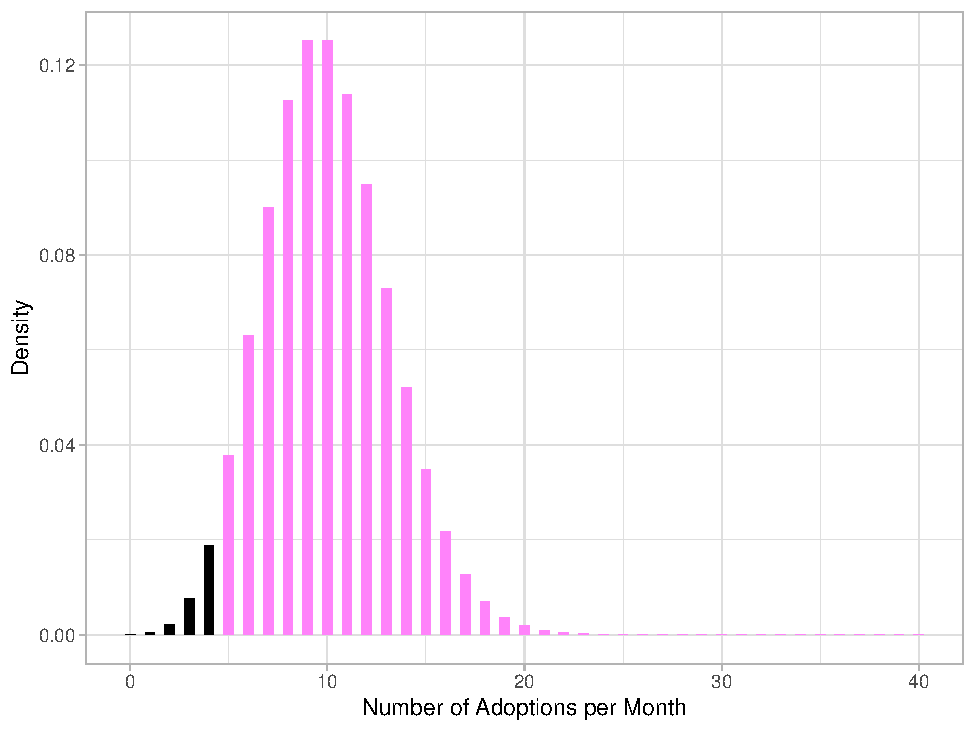
\includegraphics[width=0.8\linewidth]{famousdistrib_files/figure-latex/adoptions-plot-1} \end{center}

As we have established, the probability mass function for a poisson distribution has a mean of \(E(K) = \lambda\). The above plot seems to agree with this, since the distribution is roughly symmetric about 10.

The \textbf{standard deviation} of a poisson distribution is \(\sqrt{\lambda}\). In this case, one standard deviation would be \(\sqrt{10}\approx3.16\).

How does the distribution change as we manipulate our parameter \(\lambda\)? Applied to our example, how do the overall spread of adoptions change as the average number of adoptions change per month?

\begin{Shaded}
\begin{Highlighting}[]
\NormalTok{pois\_plot }\OtherTok{\textless{}{-}} \ControlFlowTok{function}\NormalTok{(x, lambda)\{}
\NormalTok{  temp }\OtherTok{\textless{}{-}} \FunctionTok{tibble}\NormalTok{(}\AttributeTok{num\_adopt =}\NormalTok{ x,}
                 \AttributeTok{density =} \FunctionTok{dpois}\NormalTok{(x, lambda),}
                 \AttributeTok{cume\_density =} \FunctionTok{cumsum}\NormalTok{(density))}
\NormalTok{  plot }\OtherTok{\textless{}{-}} \FunctionTok{ggplot}\NormalTok{(temp, }\FunctionTok{aes}\NormalTok{(}\AttributeTok{x =}\NormalTok{ num\_adopt, }\AttributeTok{y =}\NormalTok{ density)) }\SpecialCharTok{+}
    \FunctionTok{geom\_bar}\NormalTok{(}\AttributeTok{stat =} \StringTok{"identity"}\NormalTok{, }\AttributeTok{width =} \FloatTok{0.2}\NormalTok{) }\SpecialCharTok{+}
    \FunctionTok{labs}\NormalTok{(}\AttributeTok{x =} \ConstantTok{NULL}\NormalTok{, }\AttributeTok{y =} \ConstantTok{NULL}\NormalTok{)}
  \FunctionTok{return}\NormalTok{(plot)}
\NormalTok{\}}

\NormalTok{adoptplot\_1 }\OtherTok{\textless{}{-}} \FunctionTok{pois\_plot}\NormalTok{(}\DecValTok{0}\SpecialCharTok{:}\DecValTok{40}\NormalTok{, }\DecValTok{2}\NormalTok{) }\SpecialCharTok{+}
  \FunctionTok{ggtitle}\NormalTok{(}\StringTok{"Lambda = 2"}\NormalTok{)}
\NormalTok{adoptplot\_2 }\OtherTok{\textless{}{-}} \FunctionTok{pois\_plot}\NormalTok{(}\DecValTok{0}\SpecialCharTok{:}\DecValTok{40}\NormalTok{, }\DecValTok{3}\NormalTok{) }\SpecialCharTok{+}
  \FunctionTok{ggtitle}\NormalTok{(}\StringTok{"Lambda = 3"}\NormalTok{)}
\NormalTok{adoptplot\_3 }\OtherTok{\textless{}{-}} \FunctionTok{pois\_plot}\NormalTok{(}\DecValTok{0}\SpecialCharTok{:}\DecValTok{40}\NormalTok{, }\DecValTok{5}\NormalTok{) }\SpecialCharTok{+}
  \FunctionTok{ggtitle}\NormalTok{(}\StringTok{"Lambda = 5"}\NormalTok{)}
\NormalTok{adoptplot\_4 }\OtherTok{\textless{}{-}} \FunctionTok{pois\_plot}\NormalTok{(}\DecValTok{0}\SpecialCharTok{:}\DecValTok{40}\NormalTok{, }\DecValTok{10}\NormalTok{) }\SpecialCharTok{+}
  \FunctionTok{labs}\NormalTok{(}\AttributeTok{title =} \StringTok{"Lambda = 10"}\NormalTok{, }\AttributeTok{x =} \StringTok{"Number of Adoptions"}\NormalTok{, }\AttributeTok{y =} \StringTok{"Density"}\NormalTok{)}

\FunctionTok{plot\_grid}\NormalTok{(}\ConstantTok{NULL}\NormalTok{, adoptplot\_4, }\ConstantTok{NULL}\NormalTok{, adoptplot\_1, adoptplot\_2, adoptplot\_3, }\AttributeTok{nrow =} \DecValTok{2}\NormalTok{, }\AttributeTok{ncol =} \DecValTok{3}\NormalTok{)}
\end{Highlighting}
\end{Shaded}

\begin{center}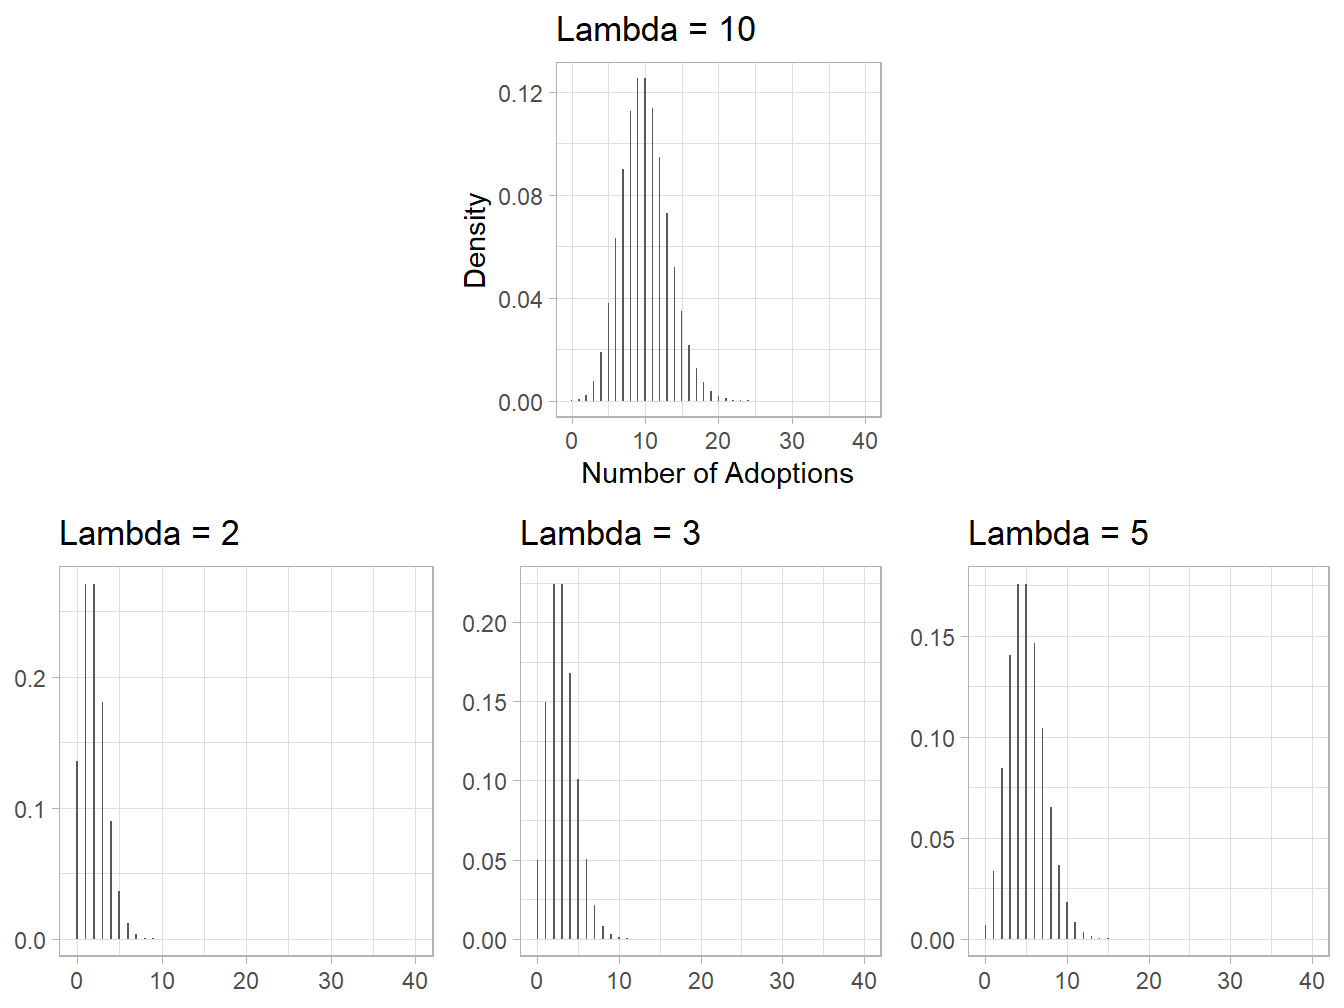
\includegraphics[width=0.8\linewidth]{famousdistrib_files/figure-latex/pois-plot-1} \end{center}

As you can see, the poisson distribution becomes more symmetric as \(\lambda\) increases. When \(\lambda\) is relatively small, the distribution is more right-skewed.

\hypertarget{DiscreteContinuous}{%
\section{From Discrete to Continuous Cases}\label{DiscreteContinuous}}

\hypertarget{normal-approximation-and-demoivres-problem}{%
\subsection{Normal Approximation and DeMoivre's Problem}\label{normal-approximation-and-demoivres-problem}}

In a way, the binomial distribution is the parent of the normal distribution. I'll explain.

Several centuries ago, mathematician Abraham DeMoivre was asked to solve a gambling problem requiring him to flip a coin many times and counts the total number of heads. After repeatedly playing the game, he found that his results resembled a unique bellcurve shape.

In this section, we will simulate his experiment:

\begin{itemize}
\tightlist
\item
  First, we will use R to create a coin. The heads side of our fair coin will be represented with a ``H'' and tails with a ``T''.
\end{itemize}

\begin{Shaded}
\begin{Highlighting}[]
\NormalTok{coin }\OtherTok{\textless{}{-}} \FunctionTok{c}\NormalTok{(}\StringTok{"H"}\NormalTok{,}\StringTok{"T"}\NormalTok{)}
\end{Highlighting}
\end{Shaded}

\begin{itemize}
\tightlist
\item
  Next, we will use \texttt{sample} to simulate random coin flips. The first argument of the function is for the elements of our random sampling process. The second \texttt{size} is the number of times that we will flip the coin. Finally, we will set \texttt{replace} to \texttt{TRUE} so that we keep both sides of our coin after flipping.
\end{itemize}

\begin{Shaded}
\begin{Highlighting}[]
\NormalTok{flips }\OtherTok{\textless{}{-}} \FunctionTok{tibble}\NormalTok{(}\AttributeTok{flip\_num =} \DecValTok{1}\SpecialCharTok{:}\DecValTok{3600}\NormalTok{, }
                \AttributeTok{outcome =} \FunctionTok{sample}\NormalTok{(coin, }\AttributeTok{size =} \DecValTok{3600}\NormalTok{, }\AttributeTok{replace =} \ConstantTok{TRUE}\NormalTok{))}

\FunctionTok{head}\NormalTok{(flips, }\DecValTok{5}\NormalTok{)}
\end{Highlighting}
\end{Shaded}

\begin{verbatim}
## # A tibble: 5 x 2
##   flip_num outcome
##      <int> <chr>  
## 1        1 T      
## 2        2 H      
## 3        3 T      
## 4        4 H      
## 5        5 H
\end{verbatim}

\begin{itemize}
\tightlist
\item
  Now, let's save the total number of heads.
\end{itemize}

\begin{Shaded}
\begin{Highlighting}[]
\NormalTok{heads }\OtherTok{\textless{}{-}}\NormalTok{ flips }\SpecialCharTok{\%\textgreater{}\%} 
  \FunctionTok{filter}\NormalTok{(outcome }\SpecialCharTok{==} \StringTok{"H"}\NormalTok{) }\SpecialCharTok{\%\textgreater{}\%} 
  \FunctionTok{count}\NormalTok{()}

\NormalTok{heads}
\end{Highlighting}
\end{Shaded}

\begin{verbatim}
## # A tibble: 1 x 1
##       n
##   <int>
## 1  1794
\end{verbatim}

\begin{itemize}
\tightlist
\item
  Our last step is to find a way to repeat this game of 3600 flips. We will do so by creating a function.
\end{itemize}

\begin{Shaded}
\begin{Highlighting}[]
\NormalTok{get\_heads }\OtherTok{\textless{}{-}} \ControlFlowTok{function}\NormalTok{() \{}
\NormalTok{  fair\_coin }\OtherTok{\textless{}{-}} \FunctionTok{c}\NormalTok{(}\StringTok{"H"}\NormalTok{, }\StringTok{"T"}\NormalTok{) }\CommentTok{\# Repeating code from the previous lines.}
\NormalTok{  flip }\OtherTok{\textless{}{-}} \FunctionTok{tibble}\NormalTok{(}\AttributeTok{flip\_num =} \DecValTok{1}\SpecialCharTok{:}\DecValTok{3600}\NormalTok{, }
                 \AttributeTok{outcome =} \FunctionTok{sample}\NormalTok{(fair\_coin, }\AttributeTok{size =} \DecValTok{3600}\NormalTok{, }\AttributeTok{replace =} \ConstantTok{TRUE}\NormalTok{))}
\NormalTok{  heads\_count }\OtherTok{\textless{}{-}}\NormalTok{ flip }\SpecialCharTok{\%\textgreater{}\%} \FunctionTok{filter}\NormalTok{(outcome }\SpecialCharTok{==} \StringTok{"H"}\NormalTok{) }\SpecialCharTok{\%\textgreater{}\%} \FunctionTok{count}\NormalTok{()}
  \FunctionTok{return}\NormalTok{(heads\_count)}
\NormalTok{\}}
\end{Highlighting}
\end{Shaded}

\begin{itemize}
\tightlist
\item
  Using this function, we will repeat the coin flip game 1000 times and count the number of heads using \texttt{replicate}. Read more about the function's documentation by typing \texttt{?replicate} into the console.
\end{itemize}

\begin{Shaded}
\begin{Highlighting}[]
\NormalTok{outcomes }\OtherTok{\textless{}{-}} \FunctionTok{tibble}\NormalTok{(}\AttributeTok{game\_num =} \DecValTok{1}\SpecialCharTok{:}\DecValTok{1000}\NormalTok{,}
                   \AttributeTok{heads =} \FunctionTok{as.numeric}\NormalTok{(}\FunctionTok{replicate}\NormalTok{(}\DecValTok{1000}\NormalTok{, }\FunctionTok{get\_heads}\NormalTok{(), }\AttributeTok{simplify =} \ConstantTok{TRUE}\NormalTok{))) }

\FunctionTok{head}\NormalTok{(outcomes, }\DecValTok{5}\NormalTok{)}
\end{Highlighting}
\end{Shaded}

\begin{verbatim}
## # A tibble: 5 x 2
##   game_num heads
##      <int> <dbl>
## 1        1  1803
## 2        2  1790
## 3        3  1831
## 4        4  1855
## 5        5  1806
\end{verbatim}

\begin{itemize}
\tightlist
\item
  What does this look like? We will first save a ggplot object called \texttt{demoivre\_plot} and then make a histogram.
\end{itemize}

\begin{Shaded}
\begin{Highlighting}[]
\CommentTok{\# Plotting our game outcomes}

\NormalTok{demoivre\_plot }\OtherTok{\textless{}{-}} \FunctionTok{ggplot}\NormalTok{(outcomes, }\FunctionTok{aes}\NormalTok{(}\AttributeTok{x =}\NormalTok{ heads))}
  
\NormalTok{demoivre\_plot }\SpecialCharTok{+}
  \FunctionTok{geom\_histogram}\NormalTok{(}\AttributeTok{bins =} \DecValTok{25}\NormalTok{) }\SpecialCharTok{+}
  \FunctionTok{labs}\NormalTok{(}\AttributeTok{x =} \StringTok{"Heads"}\NormalTok{, }\AttributeTok{y =} \StringTok{"Count"}\NormalTok{)}
\end{Highlighting}
\end{Shaded}

\textbackslash begin\{figure\}

\{\centering 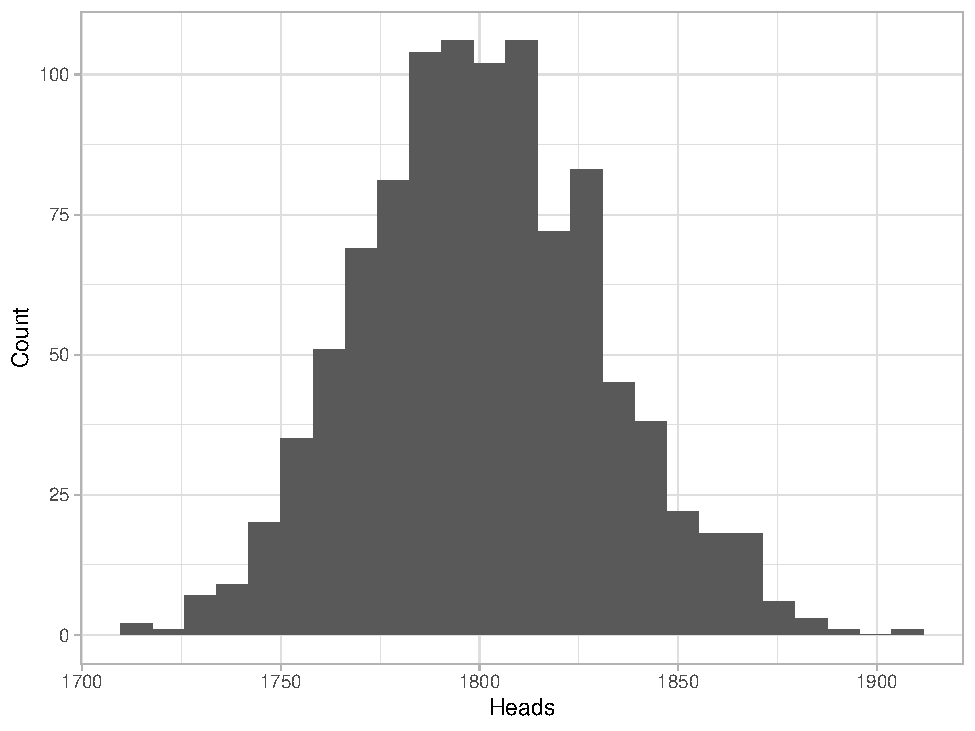
\includegraphics[width=0.6\linewidth]{famousdistrib_files/figure-latex/coinplot-hist-1}

\}

\textbackslash caption\{Coin game simulation with geom\_histogram\}\label{fig:coinplot-hist}
\textbackslash end\{figure\}

You can start to see the bell shape taking form in Figure \ref{fig:coinplot-hist}. However, this is even easier to see with \texttt{geom\_density()} which takes the same aesthetic mapping as \texttt{geom\_histogram}.

\begin{Shaded}
\begin{Highlighting}[]
\NormalTok{demoivre\_plot }\SpecialCharTok{+}
  \FunctionTok{geom\_density}\NormalTok{(}\AttributeTok{alpha =} \FloatTok{0.4}\NormalTok{, }\AttributeTok{fill =} \StringTok{"lightsteelblue"}\NormalTok{) }\SpecialCharTok{+}
  \FunctionTok{labs}\NormalTok{(}\AttributeTok{x =} \StringTok{"Heads"}\NormalTok{, }\AttributeTok{y =} \StringTok{"Density"}\NormalTok{)}
\end{Highlighting}
\end{Shaded}

\textbackslash begin\{figure\}

\{\centering 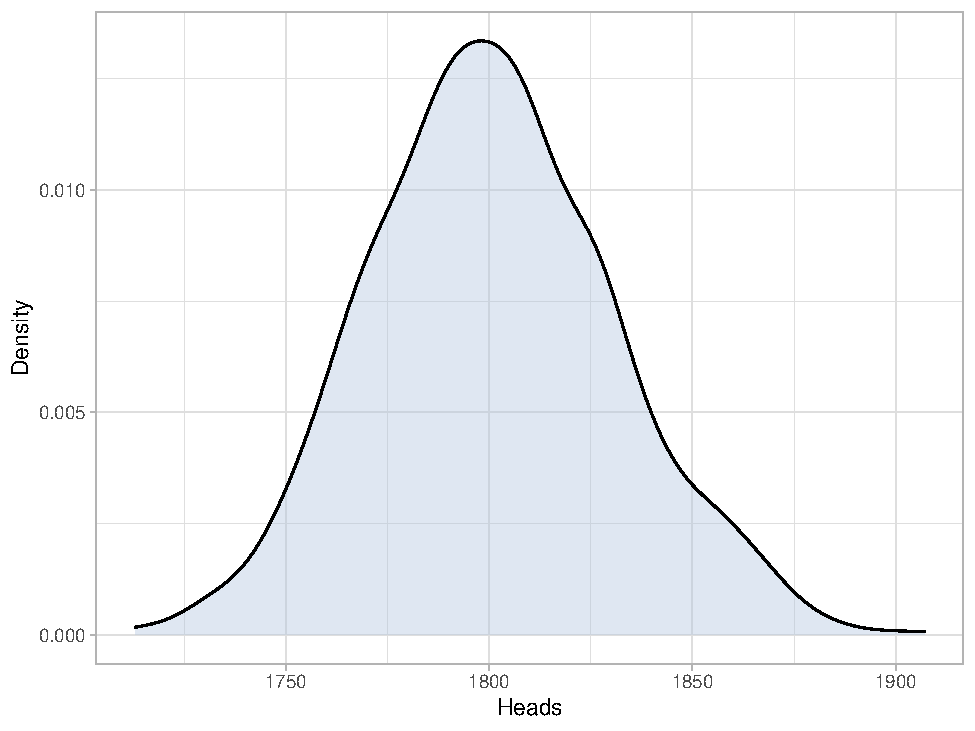
\includegraphics[width=0.6\linewidth]{famousdistrib_files/figure-latex/coinplot-density-1}

\}

\textbackslash caption\{Coin game simulation with geom\_density\}\label{fig:coinplot-density}
\textbackslash end\{figure\}

This unique bellcurve roughly follows the \textbf{normal distribution}.

This distribution is useful beyond the coin flipping game. It is also resembles many everyday phenomena such as heights, IQ scores, salaries, and blood pressure. Because of this, when we know that an outcomes, people, or observations are independent and normally distributed, we can make \emph{inferences} about the larger picture.

\begin{center}\rule{0.5\linewidth}{0.5pt}\end{center}

\hypertarget{normal-distribution}{%
\subsection{Normal Distribution}\label{normal-distribution}}

Now let's return to the normal distribution. We can define it as follows:

\[f(x)=(2\pi)^{-1/2}e^{-x^2/2} \quad \textrm{for} \enspace -\infty < x < \infty\]

The fact that \(x\) can take non-positive and non-integer values differentiates the normal distribution from \protect\hyperlink{Discrete}{discrete distributions}. These such distributions are considered \textbf{continuous}.

The density function \texttt{dnorm(x)} can be thought of as f(x). The first argument x contains a vector of numbers that will yield their density. Let's try this with \(x = 1.5\) on a standard normal distribution. This means that the mean of the distribution is 0 and the standard deviation is 1.

How likely is it that a point would be 1.5 standard deviations above the mean?

\begin{Shaded}
\begin{Highlighting}[]
\FunctionTok{dnorm}\NormalTok{(}\FloatTok{1.5}\NormalTok{, }\AttributeTok{mean =} \DecValTok{0}\NormalTok{, }\AttributeTok{sd =} \DecValTok{1}\NormalTok{) }\CommentTok{\#The mean and sd arguments are set to these values by default.}
\end{Highlighting}
\end{Shaded}

\begin{verbatim}
## [1] 0.1295176
\end{verbatim}

To interpret this density, simply think of 13\% as the probability that an observation would be 1.5 standard deviations greater than a mean.

There are many real world scenarios in which we could apply this. For instance, the probability of an American male having a height that is 1.5 standard deviations greater than average (i.e.~76 inches or 6 feet and 3 inches) is about 13\%.

\begin{center}\rule{0.5\linewidth}{0.5pt}\end{center}

Oftentimes, we don't have a standardized distribution with 0 as the mean and 1 as the standard deviation. To demonstrate this, we'll return to our height example. The average height of men in the United States is 70 inches with 2 inches as the standard deviation. Thus, we must reevaluate the \texttt{mean} and \texttt{sd} arguments.

\begin{Shaded}
\begin{Highlighting}[]
\NormalTok{normal }\OtherTok{\textless{}{-}} \FunctionTok{list}\NormalTok{(}\AttributeTok{mean =} \DecValTok{70}\NormalTok{, }\AttributeTok{sd =} \DecValTok{2}\NormalTok{)}
\end{Highlighting}
\end{Shaded}

We can visualize this differently than discrete distributions. \texttt{stat\_function} is a unique tool within ggplot that plots continuous curves. There are several required arguments:

\begin{enumerate}
\def\labelenumi{\arabic{enumi}.}
\tightlist
\item
  a geometry such as ``function'', ``point'', ``area,'' etc.,
\item
  a continuous function,
\item
  lower and upper limits on the x and/or x axis,
\item
  and a list of arguments for the function.
\end{enumerate}

We listed our arguments for a normal curve above. After plotting this curve, we will add a vertical line at the mean using \texttt{geom\_vline}. For this geometry, we are required to provide an x-intercept.

\begin{Shaded}
\begin{Highlighting}[]
\NormalTok{normal\_plot }\OtherTok{\textless{}{-}} \FunctionTok{ggplot}\NormalTok{() }\SpecialCharTok{+}
  \FunctionTok{stat\_function}\NormalTok{(}
    \AttributeTok{geom =} \StringTok{"function"}\NormalTok{,}
    \AttributeTok{fun =}\NormalTok{ dnorm,}
    \AttributeTok{xlim =} \FunctionTok{c}\NormalTok{(}\DecValTok{61}\NormalTok{, }\DecValTok{79}\NormalTok{),}
    \AttributeTok{args =}\NormalTok{ normal }\CommentTok{\# This is the list of arguments from above}
\NormalTok{  ) }\SpecialCharTok{+}
  \FunctionTok{geom\_vline}\NormalTok{(}\AttributeTok{xintercept =} \DecValTok{70}\NormalTok{, }\AttributeTok{color =} \StringTok{"lightsteelblue"}\NormalTok{, }\AttributeTok{linetype =} \StringTok{"dashed"}\NormalTok{) }\SpecialCharTok{+}
  \FunctionTok{labs}\NormalTok{(}\AttributeTok{x =} \StringTok{"Height (inches)"}\NormalTok{, }\AttributeTok{y =} \StringTok{"Density"}\NormalTok{)}

\NormalTok{normal\_plot}
\end{Highlighting}
\end{Shaded}

\begin{figure}

{\centering 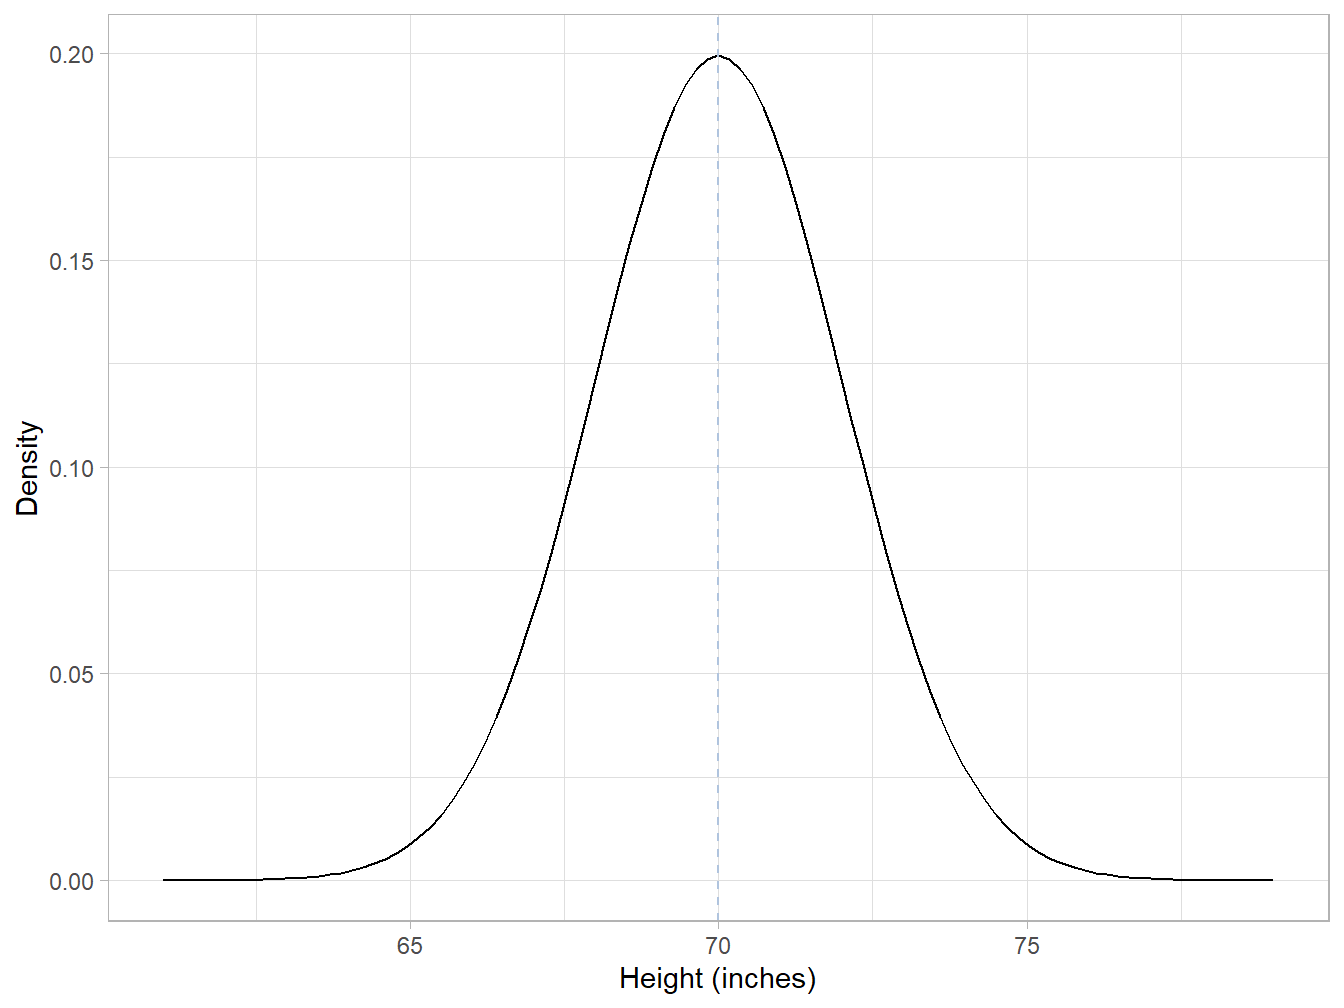
\includegraphics[width=0.6\linewidth]{famousdistrib_files/figure-latex/normal-plot-1} 

}

\caption{Normal distribution of U.S. male heights}\label{fig:normal-plot}
\end{figure}

Unlike the geometric and binomial distributions, the normal distribution is symmetric about the mean. When a height is much greater or smaller than the average, it is less likely to occur.

\begin{center}\rule{0.5\linewidth}{0.5pt}\end{center}

Now that we have made our density plot, we can again capture an interval of values in the distribution with our ``p'' distribution function \texttt{pnorm()}. If the shortest Duke basketball player (in the 2020-21 season) is 6 feet or 72 inches tall, what percentage of the American male population is shorter than the basketball team?

\begin{Shaded}
\begin{Highlighting}[]
\FunctionTok{round}\NormalTok{(}\FunctionTok{pnorm}\NormalTok{(}\DecValTok{72}\NormalTok{, }\DecValTok{70}\NormalTok{, }\DecValTok{2}\NormalTok{), }\AttributeTok{digits =} \DecValTok{3}\NormalTok{) }\SpecialCharTok{*} \DecValTok{100} \CommentTok{\# Multiply by 100 to get a percentage}
\end{Highlighting}
\end{Shaded}

\begin{verbatim}
## [1] 84.1
\end{verbatim}

To understand what the lower 84.1\% of the normal distribution looks like, we will create two geometries with \texttt{stat\_function} in Figure \ref{fig:pnorm-plot}. The first will shade the entire distribution gray. On top of that, the second \texttt{stat\_function} geometry fills the area of the distribution lower than 72 inches blue.

\begin{Shaded}
\begin{Highlighting}[]
\FunctionTok{ggplot}\NormalTok{() }\SpecialCharTok{+}
  \FunctionTok{stat\_function}\NormalTok{(}\AttributeTok{fun =}\NormalTok{ dnorm, }\CommentTok{\# Plot the entire distribution}
                \AttributeTok{geom =} \StringTok{"area"}\NormalTok{,}
                \AttributeTok{fill =} \StringTok{"lightgray"}\NormalTok{,}
                \AttributeTok{color =} \StringTok{"black"}\NormalTok{,}
                \AttributeTok{xlim =} \FunctionTok{c}\NormalTok{(}\DecValTok{61}\NormalTok{, }\DecValTok{79}\NormalTok{),}
                \AttributeTok{args =}\NormalTok{ normal) }\SpecialCharTok{+}
  \FunctionTok{stat\_function}\NormalTok{(}\AttributeTok{fun =}\NormalTok{ dnorm, }\CommentTok{\# Change the color of heights \textless{} 72 inches.}
                \AttributeTok{geom =} \StringTok{"area"}\NormalTok{,}
                \AttributeTok{fill =} \StringTok{"steelblue"}\NormalTok{,}
                \AttributeTok{xlim =} \FunctionTok{c}\NormalTok{(}\DecValTok{61}\NormalTok{, }\DecValTok{72}\NormalTok{),}
                \AttributeTok{args =}\NormalTok{ normal}
\NormalTok{                ) }\SpecialCharTok{+}
  \FunctionTok{labs}\NormalTok{(}\AttributeTok{x =} \StringTok{"Height (inches)"}\NormalTok{, }\AttributeTok{y =} \StringTok{"Density"}\NormalTok{)}
\end{Highlighting}
\end{Shaded}

\begin{figure}

{\centering 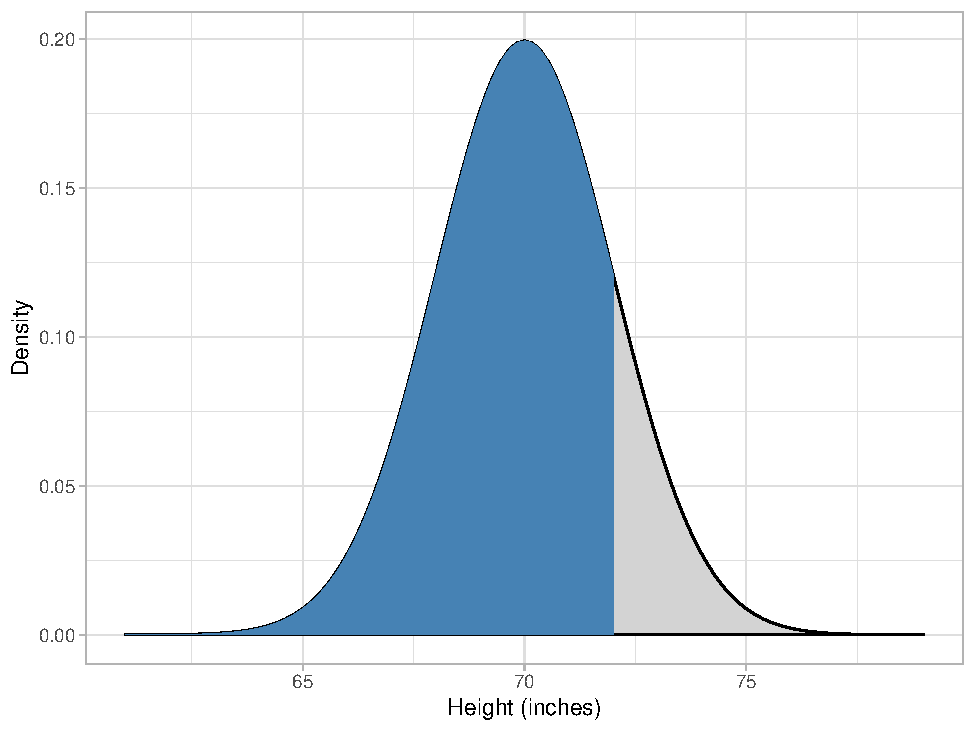
\includegraphics[width=0.6\linewidth]{famousdistrib_files/figure-latex/pnorm-plot-1} 

}

\caption{U.S. male heights below 72 inches}\label{fig:pnorm-plot}
\end{figure}

As the blue portion of the plot makes clear, a majority of American men have heights below 72 inches.

\begin{center}\rule{0.5\linewidth}{0.5pt}\end{center}

We use \texttt{rnorm} whenever we want to draw random samples from the normal distribution. On its own, the function helps us better understand the natural variation of real world processes that draw from normal distributions. If we repeat this sampling many times, we'll have a plot that more closely resembles the \emph{true} distribution.

Let's apply this concept again to height. Imagine that you took a random sample of 50 US men and took their height.

\begin{Shaded}
\begin{Highlighting}[]
\CommentTok{\# Take sample}
\NormalTok{sample\_50 }\OtherTok{\textless{}{-}} \FunctionTok{tibble}\NormalTok{(}\AttributeTok{deviates =} \FunctionTok{rnorm}\NormalTok{(}\DecValTok{50}\NormalTok{, }\DecValTok{70}\NormalTok{, }\DecValTok{2}\NormalTok{))}

\CommentTok{\# Plot as a histogram}
\FunctionTok{ggplot}\NormalTok{(sample\_50, }\FunctionTok{aes}\NormalTok{(}\AttributeTok{x =}\NormalTok{ deviates)) }\SpecialCharTok{+}
  \FunctionTok{geom\_histogram}\NormalTok{(}\AttributeTok{bins =} \DecValTok{20}\NormalTok{)}
\end{Highlighting}
\end{Shaded}

\begin{figure}

{\centering 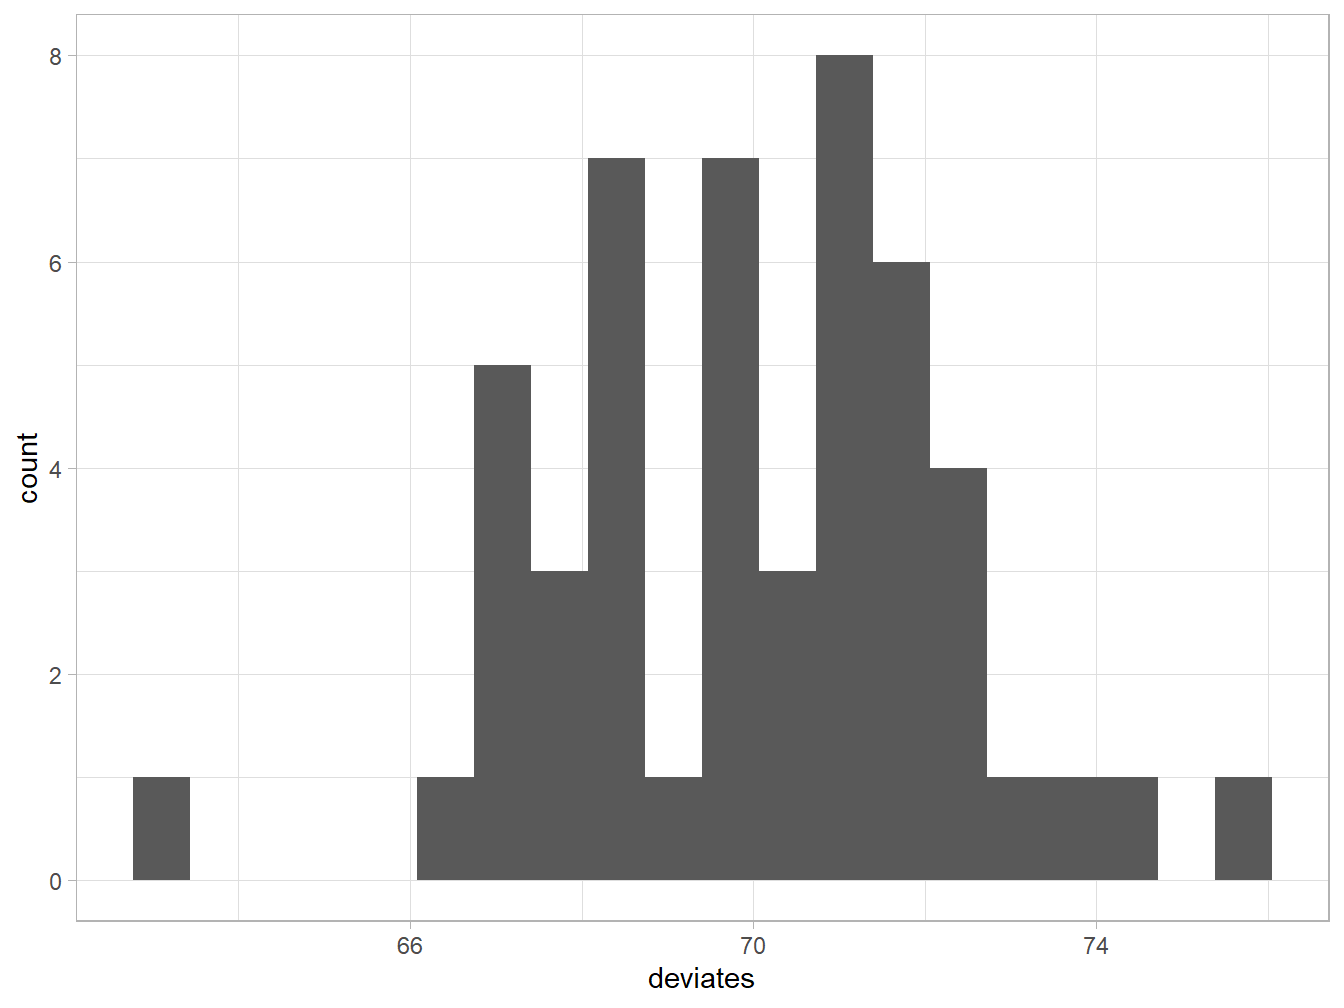
\includegraphics[width=0.6\linewidth]{famousdistrib_files/figure-latex/sample-heights-1} 

}

\caption{Heights of U.S. men, n = 50}\label{fig:sample-heights}
\end{figure}

If we took a larger sample, we would get something that looks more normally distributed.

\begin{Shaded}
\begin{Highlighting}[]
\NormalTok{sample\_5000 }\OtherTok{\textless{}{-}} \FunctionTok{tibble}\NormalTok{(}\AttributeTok{deviates =} \FunctionTok{rnorm}\NormalTok{(}\DecValTok{5000}\NormalTok{, }\DecValTok{70}\NormalTok{, }\DecValTok{2}\NormalTok{))}

\FunctionTok{ggplot}\NormalTok{(sample\_5000, }\FunctionTok{aes}\NormalTok{(}\AttributeTok{x =}\NormalTok{ deviates)) }\SpecialCharTok{+}
  \FunctionTok{geom\_histogram}\NormalTok{(}\AttributeTok{bins =} \DecValTok{20}\NormalTok{)}
\end{Highlighting}
\end{Shaded}

\begin{figure}

{\centering 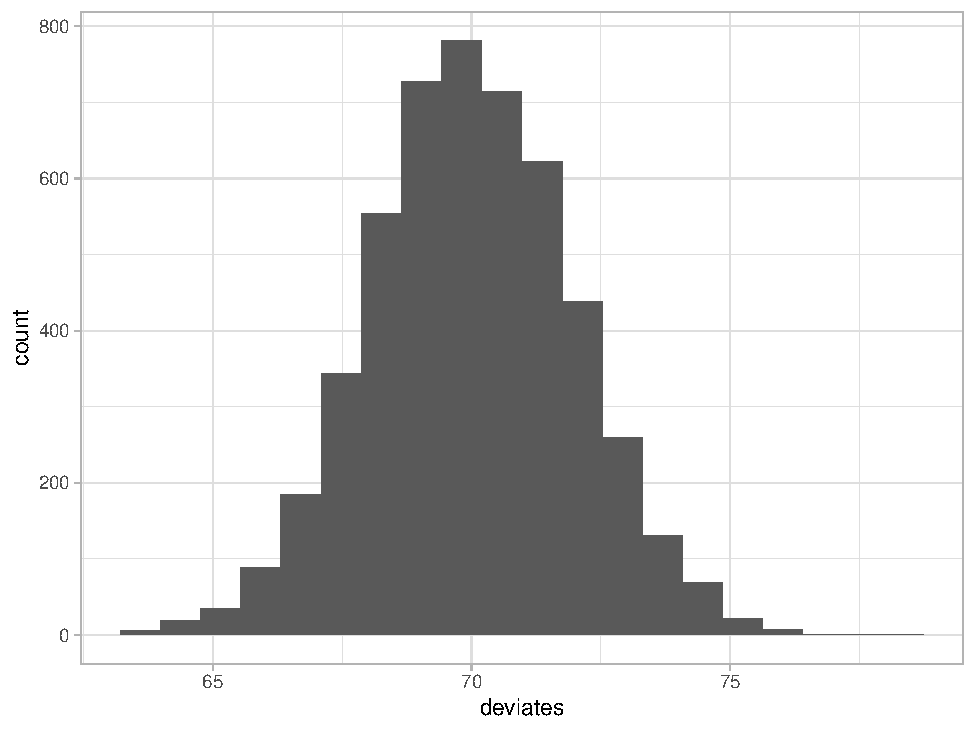
\includegraphics[width=0.6\linewidth]{famousdistrib_files/figure-latex/large-sample-1} 

}

\caption{Heights of U.S. men, n = 5000}\label{fig:large-sample}
\end{figure}

The plots below will more finely measure this progression as sample sizes increase:

\begin{Shaded}
\begin{Highlighting}[]
\CommentTok{\# Create a function that randomly samples from normal distribution}
\NormalTok{norm\_plot }\OtherTok{\textless{}{-}} \ControlFlowTok{function}\NormalTok{(mean, sd, n)\{}
\NormalTok{  temp }\OtherTok{\textless{}{-}} \FunctionTok{tibble}\NormalTok{(}\AttributeTok{deviates =} \FunctionTok{rnorm}\NormalTok{(n, mean, sd))}
\NormalTok{  plot }\OtherTok{\textless{}{-}} \FunctionTok{ggplot}\NormalTok{(temp, }\FunctionTok{aes}\NormalTok{(}\AttributeTok{x =}\NormalTok{ deviates)) }\SpecialCharTok{+}
    \FunctionTok{geom\_histogram}\NormalTok{(}\AttributeTok{bins =} \DecValTok{20}\NormalTok{)}
  \FunctionTok{return}\NormalTok{(plot)}
\NormalTok{\}}

\CommentTok{\# Produce plots}
\NormalTok{sample\_50 }\OtherTok{\textless{}{-}} \FunctionTok{norm\_plot}\NormalTok{(}\DecValTok{70}\NormalTok{, }\DecValTok{2}\NormalTok{, }\DecValTok{50}\NormalTok{)}
\NormalTok{sample\_500 }\OtherTok{\textless{}{-}} \FunctionTok{norm\_plot}\NormalTok{(}\DecValTok{70}\NormalTok{, }\DecValTok{2}\NormalTok{, }\DecValTok{500}\NormalTok{)}
\NormalTok{sample\_5000 }\OtherTok{\textless{}{-}} \FunctionTok{norm\_plot}\NormalTok{(}\DecValTok{70}\NormalTok{, }\DecValTok{2}\NormalTok{, }\DecValTok{5000}\NormalTok{)}

\CommentTok{\# Plot together}
\NormalTok{cowplot}\SpecialCharTok{::}\FunctionTok{plot\_grid}\NormalTok{(}\ConstantTok{NULL}\NormalTok{, normal\_plot, }\ConstantTok{NULL}\NormalTok{, sample\_50, sample\_500, sample\_5000, }\AttributeTok{ncol =} \DecValTok{3}\NormalTok{, }\AttributeTok{nrow =} \DecValTok{2}\NormalTok{)}
\end{Highlighting}
\end{Shaded}

\begin{figure}

{\centering 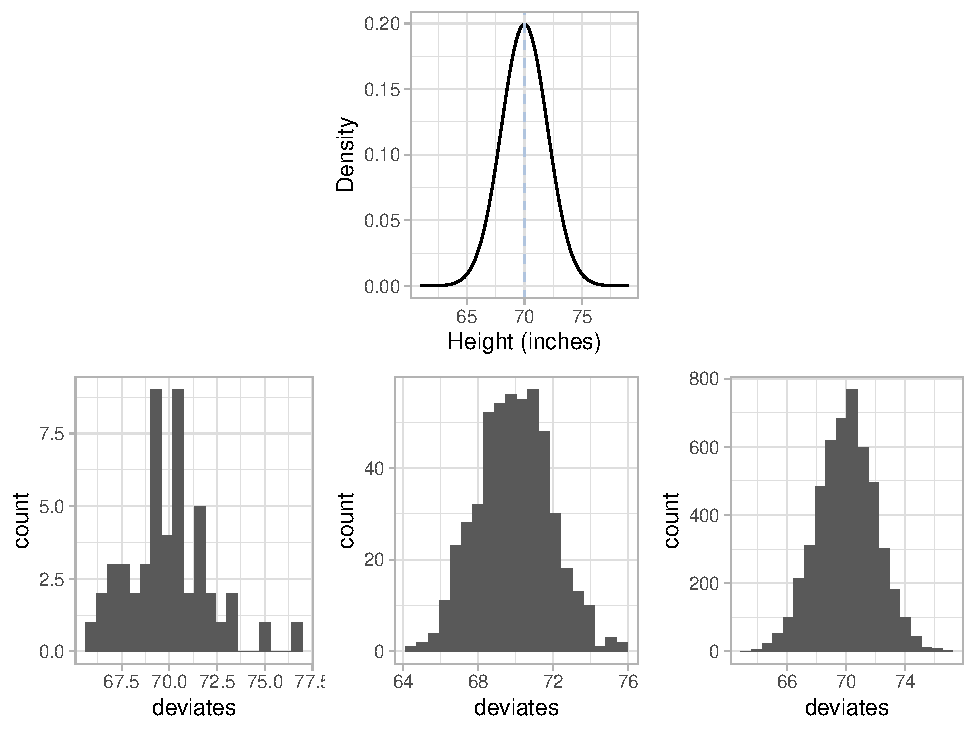
\includegraphics[width=0.6\linewidth]{famousdistrib_files/figure-latex/samples-comp-1} 

}

\caption{Comparison of samples to normal distribution}\label{fig:samples-comp}
\end{figure}

Now that we have looked at the normal distribution, let's continue to look at other continuous random variables.

\hypertarget{Continuous}{%
\section{Other Continuous Distributions}\label{Continuous}}

\hypertarget{T}{%
\subsection{t-Distribution}\label{T}}

We often don't know the true variance (and thus the standard deviation) of normally-distributed populations. However, we can still make estimations and inferences by adding a new parameter \(t\), the \textbf{degrees of freedom}. After doing this, we have created a t-distribution. This is also known as a student's t-distribution.

Simply put, degrees of freedom comes from the number of observations in our sample that are able to, or have the \emph{freedom}, to vary given our constraints. Since the only parameter that limits the freedom of our sample is the mean, we have \(t = n-1\) degrees of freedom in a t-distribution.

Let's say that you have a sample of 5 observations: 1, 3, 5, 7, and an unknown number \(x_5\). If we know that that the mean of the data is \(\bar{x}=5\), we can conclude that \(x_5=9\) given the definition of means.

\[\begin{split} \bar{x} &= \frac{\sum_{1}^p x_i}{p} = \frac{x_1+x_2+\ldots+x_p}{p} \\
5 &= \frac{1+3+5+7+x_5}{5} \\
x_5 &= 9
\end{split}\]

In other words, if we impose the mean as a constraint on our data, all but 1 observation in our sample is able to vary. Since \(n\) is the sample size, having larger samples means more degrees of freedom.

Regardless of the degrees of freedom a t-distribution has, it will look like an approximately-normal curve with greater variability than the normal distribution when plotted. This why some describe the distribution as having thick ``tails.''

\begin{Shaded}
\begin{Highlighting}[]
\FunctionTok{ggplot}\NormalTok{() }\SpecialCharTok{+}
  \FunctionTok{geom\_function}\NormalTok{(}\AttributeTok{fun =}\NormalTok{ dt, }\AttributeTok{args =} \FunctionTok{list}\NormalTok{(}\AttributeTok{df =} \DecValTok{5}\NormalTok{), }\AttributeTok{color =} \StringTok{"darkred"}\NormalTok{) }\SpecialCharTok{+}
  \FunctionTok{xlim}\NormalTok{(}\FunctionTok{c}\NormalTok{(}\SpecialCharTok{{-}}\DecValTok{3}\NormalTok{, }\DecValTok{3}\NormalTok{)) }\SpecialCharTok{+}
  \FunctionTok{labs}\NormalTok{(}\AttributeTok{y =} \StringTok{"Density"}\NormalTok{)}
\end{Highlighting}
\end{Shaded}

\begin{figure}

{\centering 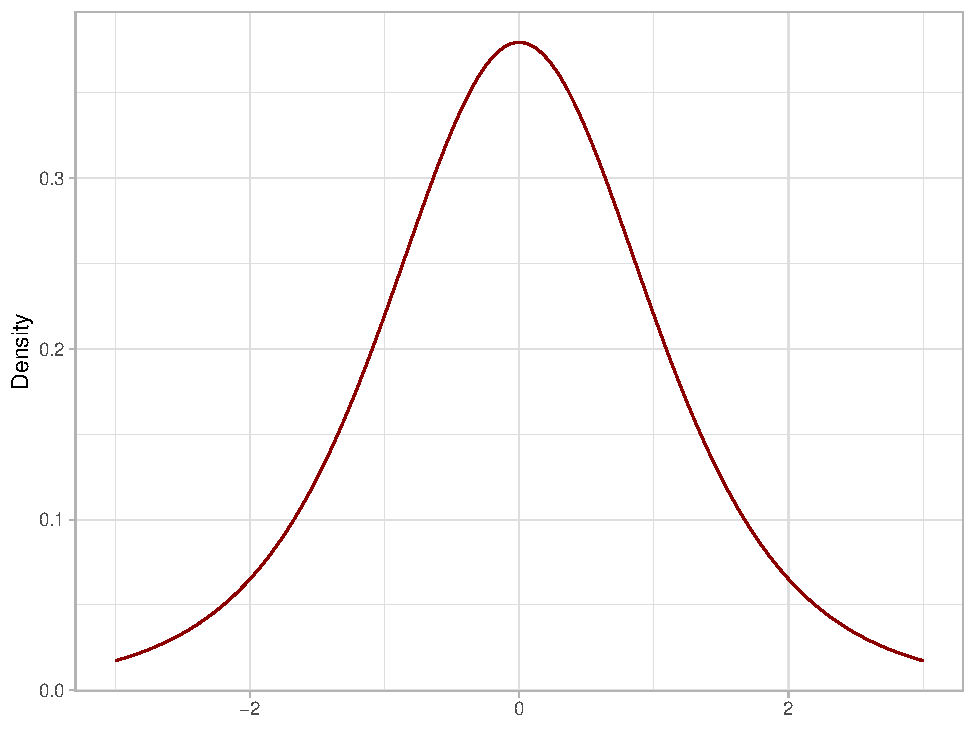
\includegraphics[width=0.8\linewidth]{famousdistrib_files/figure-latex/tplot-1} 

}

\caption{t-distribution with 5 degrees of freedom}\label{fig:tplot}
\end{figure}

I don't recommend that you use ggplot without something in the data argument since it limits your ability to alter aesthetics. However, for the purpose of simply visualizing continuous curves like the t-distribution, we can use \texttt{geom\_function}.

As you see above, we need to provide \texttt{geom\_function} a function as the first argument. \texttt{dt} is the density function for the t-distribution. By specifying the limits on the x-axis with \texttt{xlim} to -3 and 3, we isolated the visualization to the most important part of the curve.

As mentioned earlier, a t-distribution gains more degrees of freedom as the sample size increases. If we plot several curves with different degrees of freedom next to each other, we would notice that t-distributions with larger degrees of freedom have narrower tails and look closer to a normal distribution. This is because the magnitude of the last non-independent observation's effect on the mean weakens as there are more observations.

Why is this the case? Imagine that you are working for an polling firm and want to measure the public's attitudes towards a new policy. You use a \href{https://www.google.com/url?sa=t\&rct=j\&q=\&esrc=s\&source=web\&cd=\&cad=rja\&uact=8\&ved=2ahUKEwj2i9-mgujxAhUJ-Z4KHQx3DYUQFnoECAMQAA\&url=https\%3A\%2F\%2Felectionstudies.org\%2F2007anes_gallup_questioncomparisons\%2F\&usg=AOvVaw0Q8BKck04Z4eMBT0hWyUqj}{feeling thermometer} to gauge each individual's favorability on a scale from 0 to 100, where numbers higher than 50 represent favorable views.

Unless we poll every member in the public, we do not know the true mean or variance of the population's views towards the policy. Thus, we introduce the sample mean (\(\bar{x}\)) as a constraint, since we assume that random samples would accurately approximate the average person's views, given that the sample is \textbf{large enough} to be representative.

However, we must also make several other assumptions before using the t-distribution. For one, the response of poll participants must be \textbf{normally distributed} (or near normal).

As mentioned previously, the sample size must also be \textbf{large enough} to avoid randomly-produced error. Although there is no definitive cutoff, polls with larger samples are usually more accurate. The impact of each respondent's opinion on the result of the poll decreases, meaning that the variability of distribution decreases.

\begin{Shaded}
\begin{Highlighting}[]
\CommentTok{\# Remember to set seeds before random processes!}
\FunctionTok{set.seed}\NormalTok{(}\DecValTok{0}\NormalTok{)}

\CommentTok{\# Generate random samples with mean = 50, sd = 12. Larger samples produce better approximations}

\NormalTok{sample\_error }\OtherTok{\textless{}{-}} \ControlFlowTok{function}\NormalTok{(true\_mean, simulations, n) \{}
  \FunctionTok{mean}\NormalTok{(}\FunctionTok{abs}\NormalTok{(true\_mean }\SpecialCharTok{{-}} \FunctionTok{replicate}\NormalTok{(simulations, }\FunctionTok{mean}\NormalTok{(}\FunctionTok{rnorm}\NormalTok{(n, }\DecValTok{50}\NormalTok{, }\DecValTok{12}\NormalTok{)))))}
\NormalTok{\}}

\FunctionTok{tibble}\NormalTok{(}\StringTok{\textasciigrave{}}\AttributeTok{n = 2}\StringTok{\textasciigrave{}} \OtherTok{=} \FunctionTok{sample\_error}\NormalTok{(}\DecValTok{50}\NormalTok{, }\DecValTok{1000}\NormalTok{, }\DecValTok{2}\NormalTok{),}
       \StringTok{\textasciigrave{}}\AttributeTok{25}\StringTok{\textasciigrave{}} \OtherTok{=} \FunctionTok{sample\_error}\NormalTok{(}\DecValTok{50}\NormalTok{, }\DecValTok{1000}\NormalTok{, }\DecValTok{25}\NormalTok{),}
       \StringTok{\textasciigrave{}}\AttributeTok{250}\StringTok{\textasciigrave{}} \OtherTok{=} \FunctionTok{sample\_error}\NormalTok{(}\DecValTok{50}\NormalTok{, }\DecValTok{1000}\NormalTok{, }\DecValTok{250}\NormalTok{),}
\NormalTok{) }\SpecialCharTok{\%\textgreater{}\%}\NormalTok{ knitr}\SpecialCharTok{::}\FunctionTok{kable}\NormalTok{(}\AttributeTok{digits =} \DecValTok{3}\NormalTok{, }\AttributeTok{caption =} \StringTok{"Average Error of Sample Means after 1000 Simulations"}\NormalTok{)}
\end{Highlighting}
\end{Shaded}

\begin{table}

\caption{\label{tab:unnamed-chunk-4}Average Error of Sample Means after 1000 Simulations}
\centering
\begin{tabular}[t]{r|r|r}
\hline
n = 2 & 25 & 250\\
\hline
6.868 & 1.879 & 0.591\\
\hline
\end{tabular}
\end{table}

\begin{Shaded}
\begin{Highlighting}[]
\NormalTok{x }\OtherTok{\textless{}{-}} \FunctionTok{as\_vector}\NormalTok{(}\FunctionTok{c}\NormalTok{(}\DecValTok{2}\NormalTok{, }\DecValTok{25}\NormalTok{, }\DecValTok{250}\NormalTok{))}

\FunctionTok{sample\_error}\NormalTok{(}\DecValTok{50}\NormalTok{, }\DecValTok{1000}\NormalTok{, }\FunctionTok{c}\NormalTok{(}\DecValTok{2}\NormalTok{, }\DecValTok{25}\NormalTok{, }\DecValTok{250}\NormalTok{))}
\end{Highlighting}
\end{Shaded}

\begin{verbatim}
## [1] 5.570544
\end{verbatim}

The change in variability as sample sizes increase is what gives some t-distributions thinner tails. Below, we'll plot several different t-distributions with various degrees of freedom as well as a normal distribution.

\begin{Shaded}
\begin{Highlighting}[]
\CommentTok{\# Make a tibble or dataframe with five curves}

\NormalTok{df }\OtherTok{\textless{}{-}} \FunctionTok{tibble}\NormalTok{(}\AttributeTok{x =} \FunctionTok{seq}\NormalTok{(}\SpecialCharTok{{-}}\DecValTok{3}\NormalTok{, }\DecValTok{3}\NormalTok{, }\AttributeTok{by =} \FloatTok{0.001}\NormalTok{),}
             \AttributeTok{t1 =} \FunctionTok{dt}\NormalTok{(x, }\DecValTok{3}\NormalTok{),}
             \AttributeTok{t2 =} \FunctionTok{dt}\NormalTok{(x, }\DecValTok{5}\NormalTok{),}
             \AttributeTok{t3 =} \FunctionTok{dt}\NormalTok{(x, }\DecValTok{7}\NormalTok{),}
             \AttributeTok{norm =} \FunctionTok{dnorm}\NormalTok{(x)) }\SpecialCharTok{\%\textgreater{}\%} 
  \FunctionTok{pivot\_longer}\NormalTok{(}\AttributeTok{cols =} \DecValTok{2}\SpecialCharTok{:}\DecValTok{5}\NormalTok{, }\AttributeTok{names\_to =} \StringTok{"Distribution"}\NormalTok{, }\AttributeTok{values\_to =} \StringTok{"Density"}\NormalTok{) }\CommentTok{\# Transform into three columns}

\CommentTok{\# Plot}
\FunctionTok{ggplot}\NormalTok{(df, }\FunctionTok{aes}\NormalTok{(}\AttributeTok{x =}\NormalTok{ x, }\AttributeTok{y =}\NormalTok{ Density)) }\SpecialCharTok{+}
  \FunctionTok{geom\_line}\NormalTok{(}\FunctionTok{aes}\NormalTok{(}\AttributeTok{color =}\NormalTok{ Distribution)) }\SpecialCharTok{+}
  \FunctionTok{scale\_color\_viridis\_d}\NormalTok{(}\AttributeTok{labels =} \FunctionTok{c}\NormalTok{(}\StringTok{"Normal"}\NormalTok{, }\StringTok{"t, df = 3"}\NormalTok{, }\StringTok{"t, df = 5"}\NormalTok{, }\StringTok{"t, df = 7"}\NormalTok{)) }\SpecialCharTok{+}
  \FunctionTok{xlim}\NormalTok{(}\FunctionTok{c}\NormalTok{(}\SpecialCharTok{{-}}\DecValTok{3}\NormalTok{, }\DecValTok{3}\NormalTok{))}
\end{Highlighting}
\end{Shaded}

\begin{figure}

{\centering 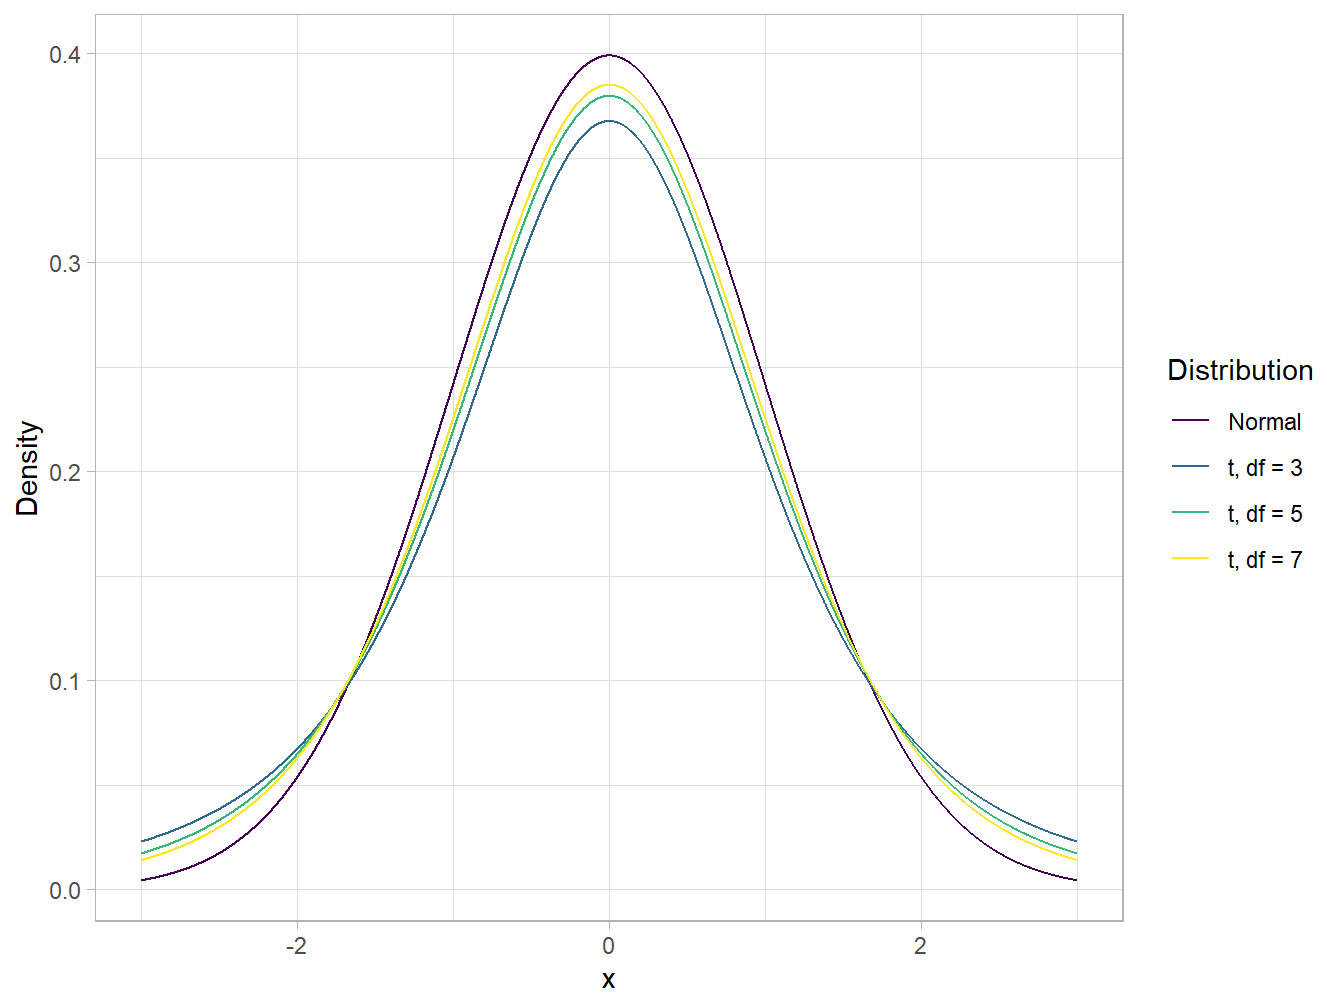
\includegraphics[width=0.8\linewidth]{famousdistrib_files/figure-latex/tplots-1} 

}

\caption{t-distributions and normal distribution}\label{fig:tplots}
\end{figure}

The concept of degrees of freedom alone can be covered more in-depth \href{https://www.google.com/url?sa=t\&rct=j\&q=\&esrc=s\&source=web\&cd=\&ved=2ahUKEwj6guTEn9zxAhWSFlkFHbpRDrcQFjAJegQIAxAD\&url=http\%3A\%2F\%2Fweb.pdx.edu\%2F~stipakb\%2Fdownload\%2FPA551\%2FDegreesOfFreedom.pdf\&usg=AOvVaw31ywhyELwYqUyDvu85-19L}{here}.

\hypertarget{Exponential}{%
\subsection{Exponential Distribution}\label{Exponential}}

Recall the earlier section in which we discussed \protect\hyperlink{Poisson}{Poisson} processes. The exponential distribution models a waiting time with \(\lambda\) as the rate. This is similar to the \protect\hyperlink{ux5cux2520geometric}{geometric} distribution, which models the number of failures until one ``success''; however, in this case, we are considering events and not successes/failures.

If \(\lambda\) is the rate of a Poisson process, the density function can be written as:

\[f(y)=\lambda e^{-\lambda y} \quad \textrm{for} \enspace y>0\]

Thus, the probability that \(Y=y\) can be interpreted as ``the likelihood that two events occurred in y units of time.''

Let's return to the adoption center example. Recall that the center has 10 adoptions per month on average. What is the probability that two pets are adopted in a week?

If each month has 30 days then people are adopting \(1/3\) of a pet each day on average (even though you can't adopt a fraction of an animal!). We can then determine the rate as \(\lambda=1/3\).

Plugging the parameter \(y<7\) and \(\lambda=1/3\):

\[\begin{split}
P(Y < 7) &= \int_{0}^{7} \frac{1}{3} e^{-1/3y}dy \\ &= \frac{1}{3} \int_{0}^{7} e^{-1/3y}dy \\ &= \frac{1}{3} [-3e^{-1/3y}]^{7}_{0} \\ &= 1-\frac{1}{e^{7/3}} \approx 0.903
\end{split}\]

Our final answer can be thought of as: ``There is a 90.3\% chance probability that two animals are adopted before the end of a week.''

If you prefer to avoid calculus, you can also use R to answer this problem using \texttt{pexp}, the corresponding distribution function.

\begin{Shaded}
\begin{Highlighting}[]
\FunctionTok{pexp}\NormalTok{(}\DecValTok{7}\NormalTok{, }\AttributeTok{rate =} \DecValTok{1}\SpecialCharTok{/}\DecValTok{3}\NormalTok{, }\AttributeTok{lower.tail =} \ConstantTok{TRUE}\NormalTok{) }\CommentTok{\# i.e. P(Y \textless{} 7) since lower.tail = TRUE}
\end{Highlighting}
\end{Shaded}

\begin{verbatim}
## [1] 0.903028
\end{verbatim}

Why can't we we simply find the the sum of the densities \texttt{1:6}? Remember that the exponential distribution is continuous, not discrete! So only calculating the individual densities at integer values would give us an underestimate.

\begin{Shaded}
\begin{Highlighting}[]
\FunctionTok{sum}\NormalTok{(}\FunctionTok{dexp}\NormalTok{(}\DecValTok{1}\SpecialCharTok{:}\DecValTok{6}\NormalTok{, }\DecValTok{1}\SpecialCharTok{/}\DecValTok{3}\NormalTok{))}
\end{Highlighting}
\end{Shaded}

\begin{verbatim}
## [1] 0.7285453
\end{verbatim}

Instead, we are required to provide an integral. To write a definite integral using R, we must provide a function and the two bounds.

\begin{Shaded}
\begin{Highlighting}[]
\NormalTok{exp\_fun }\OtherTok{\textless{}{-}} \ControlFlowTok{function}\NormalTok{(y) }\DecValTok{1}\SpecialCharTok{/}\DecValTok{3}\SpecialCharTok{*}\FunctionTok{exp}\NormalTok{(}\SpecialCharTok{{-}}\DecValTok{1}\SpecialCharTok{/}\DecValTok{3}\SpecialCharTok{*}\NormalTok{y) }\CommentTok{\# Write exponential function}
\FunctionTok{integrate}\NormalTok{(exp\_fun, }\DecValTok{0}\NormalTok{, }\DecValTok{7}\NormalTok{)}
\end{Highlighting}
\end{Shaded}

\begin{verbatim}
## 0.903028 with absolute error < 1e-14
\end{verbatim}

How can we visualize our interval between 0 and 7 days? Let's again use \texttt{stat\_function} to draw a curve.

\begin{Shaded}
\begin{Highlighting}[]
\NormalTok{exp\_correct }\OtherTok{\textless{}{-}} \FunctionTok{ggplot}\NormalTok{() }\SpecialCharTok{+}
  \FunctionTok{stat\_function}\NormalTok{(}
    \AttributeTok{fun =}\NormalTok{ dexp,}
    \AttributeTok{args =} \FunctionTok{list}\NormalTok{(}\AttributeTok{rate =} \DecValTok{1}\SpecialCharTok{/}\DecValTok{3}\NormalTok{),}
    \AttributeTok{xlim =} \FunctionTok{c}\NormalTok{(}\DecValTok{0}\NormalTok{, }\DecValTok{7}\NormalTok{),}
    \AttributeTok{geom =} \StringTok{"area"}\NormalTok{,}
    \AttributeTok{fill =} \StringTok{"skyblue1"}
\NormalTok{  ) }\SpecialCharTok{+}
  \FunctionTok{stat\_function}\NormalTok{(}
    \AttributeTok{fun =}\NormalTok{ dexp,}
    \AttributeTok{args =} \FunctionTok{list}\NormalTok{(}\AttributeTok{rate =} \DecValTok{1}\SpecialCharTok{/}\DecValTok{3}\NormalTok{), }\CommentTok{\# Remember, the arguments must be provided in a list}
    \AttributeTok{xlim =} \FunctionTok{c}\NormalTok{(}\DecValTok{0}\NormalTok{, }\DecValTok{30}\NormalTok{),}
    \AttributeTok{geom =} \StringTok{"function"}\NormalTok{, }\CommentTok{\# Choose a curve as the geometry}
    \AttributeTok{size =} \FloatTok{0.5}\NormalTok{) }\SpecialCharTok{+}
  \FunctionTok{geom\_segment}\NormalTok{(}\FunctionTok{aes}\NormalTok{(}\AttributeTok{x =} \DecValTok{0}\SpecialCharTok{:}\DecValTok{30}\NormalTok{, }\AttributeTok{y =} \DecValTok{0}\NormalTok{, }\AttributeTok{xend =} \DecValTok{0}\SpecialCharTok{:}\DecValTok{30}\NormalTok{, }\AttributeTok{yend =} \FunctionTok{dexp}\NormalTok{(}\DecValTok{0}\SpecialCharTok{:}\DecValTok{30}\NormalTok{, }\AttributeTok{rate =} \DecValTok{1}\SpecialCharTok{/}\DecValTok{3}\NormalTok{)), }\AttributeTok{size =} \FloatTok{0.5}\NormalTok{) }\SpecialCharTok{+}
  \FunctionTok{labs}\NormalTok{(}\AttributeTok{x =} \StringTok{"Days Between Adoptions"}\NormalTok{, }\AttributeTok{y =} \StringTok{"Density"}\NormalTok{)}
\end{Highlighting}
\end{Shaded}

\begin{figure}

{\centering 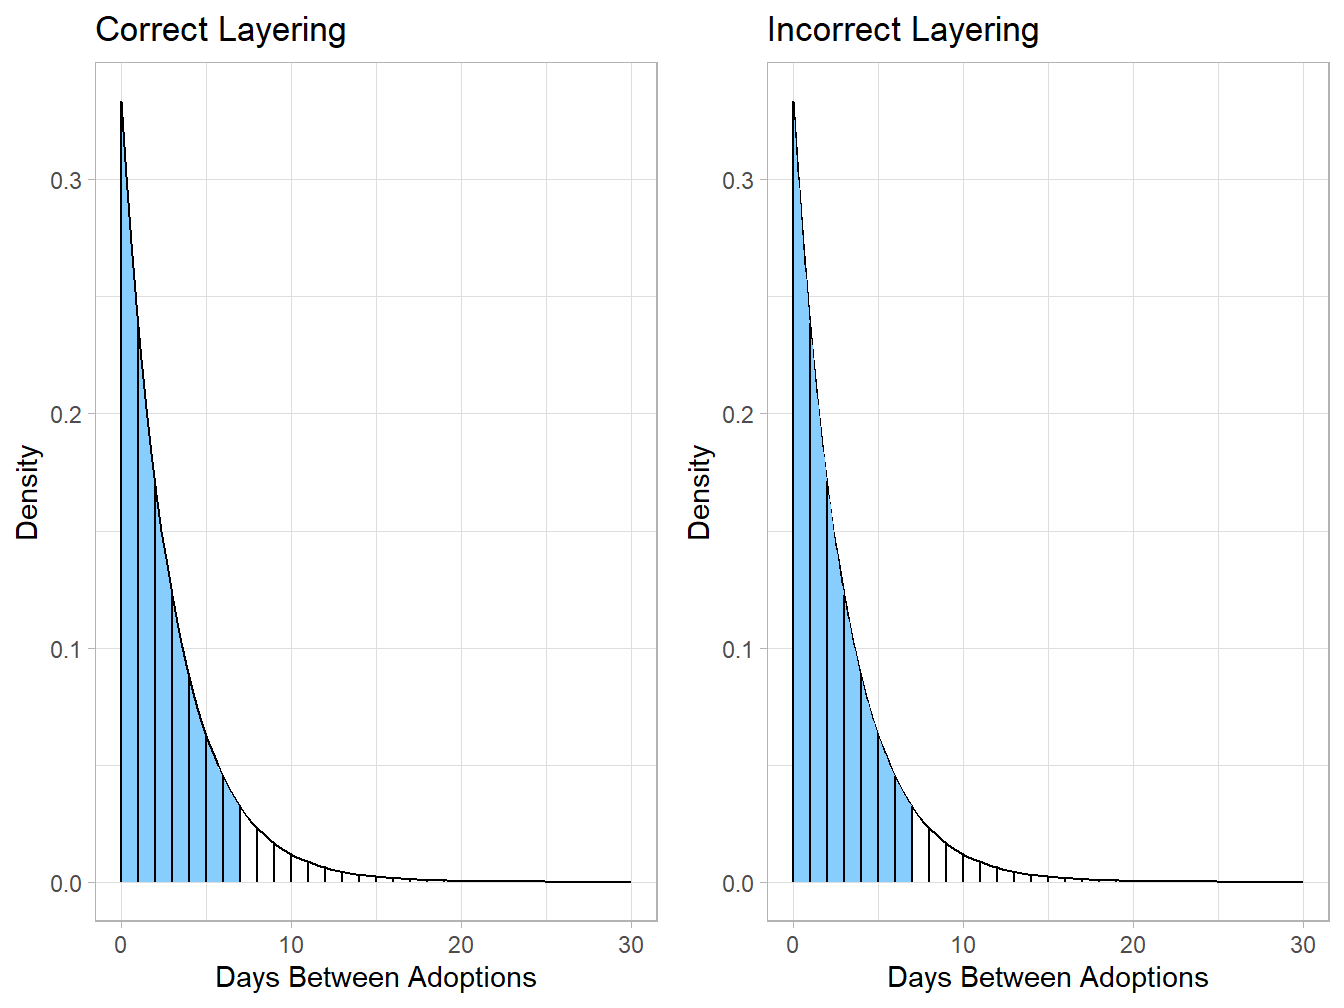
\includegraphics[width=0.6\linewidth]{famousdistrib_files/figure-latex/exp comparison-1} 

}

\caption{Correct and incorrect layering of exponential distribution layers}(\#fig:exp comparison)
\end{figure}

Notice how the plot on the left looks much better? They are also placed so that the blue fill does not cover the curve? The jagged edges on the right plot results from placing the function geometry before the area geometry.

Because a large majority of the plot below 7 is colored in, it is quite likely that 2 pets would be adopted in a week. As the number of days ``waiting'' approaches 30, the probability approaches 0.

\begin{center}\rule{0.5\linewidth}{0.5pt}\end{center}

By what point after one adoption can we begin expecting another? To answer this question, we can look for the median of the distribution.

Recall that ``q'' functions return a x-value after providing a quantile in the distribution. Here, we'll use \texttt{qexp}.

\begin{Shaded}
\begin{Highlighting}[]
\FunctionTok{qexp}\NormalTok{(}\FloatTok{0.5}\NormalTok{, }\AttributeTok{rate =} \DecValTok{1}\SpecialCharTok{/}\DecValTok{3}\NormalTok{)}
\end{Highlighting}
\end{Shaded}

\begin{verbatim}
## [1] 2.079442
\end{verbatim}

The other measure of center for an exponential distribution is the mean. This is much easier to solve; if K is a Poisson random variable, \(E(K)=\frac{1}{\lambda}\). So on average, we can expect an adoption on day \(\frac{1}{1/3}=3\).

\begin{center}\rule{0.5\linewidth}{0.5pt}\end{center}

Imagine that you are working for a rescue shelter for pets and want to present the information that you just learned--that there are about 3 days on average between any two adoptions in a month.

We'll build a deliverable visualization using the power of \texttt{ggplot}, \texttt{ggimage}, as well as your knowledge about the exponential distribution.

First, load the new \texttt{ggimage} package. This allows us to include image files and other graphic objects in our visualizations. To learn more about it, you can read ggimage's documentation \href{https://cran.r-project.org/web/packages/ggimage/index.html}{here}.

\begin{Shaded}
\begin{Highlighting}[]
\FunctionTok{library}\NormalTok{(ggimage) }\CommentTok{\# Remember to use install.packages("ggimage") first}
\end{Highlighting}
\end{Shaded}

In particular, we'll need the package to include emojis of dogs and illustrate the average time period between adoptions. Think of adding the emojis as adding any other geometry. Beyond a coordinate position, the \texttt{geom\_emoji} function requires an aesthetic called ``image.'' The special unicode required for dogs is ``1f415''. We can also set the size of the image similar to geometries like \texttt{geom\_point}.

\begin{figure}

{\centering 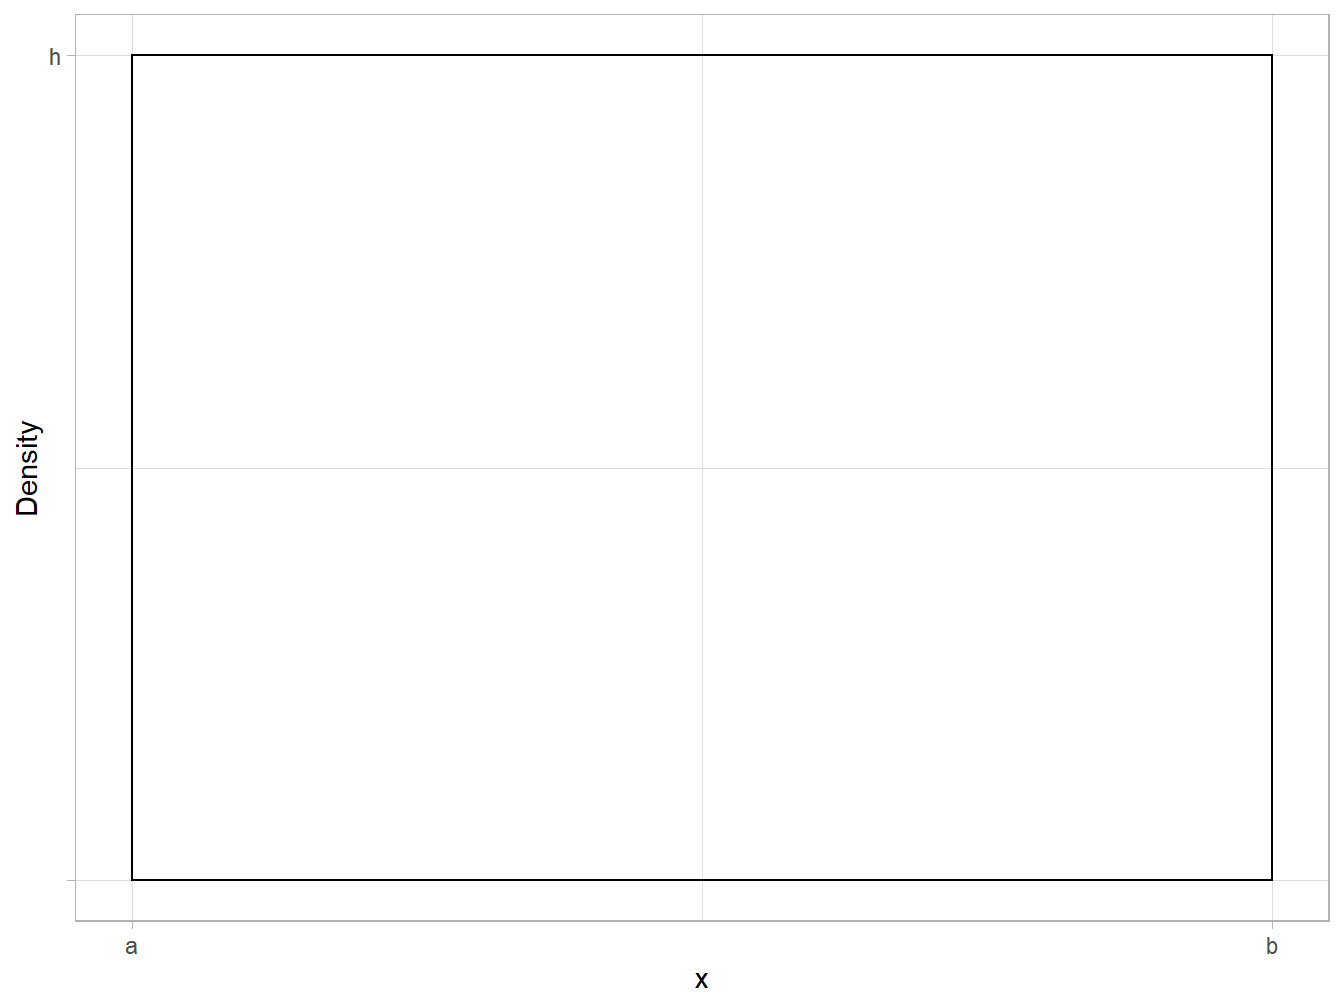
\includegraphics[width=0.2\linewidth]{famousdistrib_files/figure-latex/unnamed-chunk-5-1} 

}

\caption{Dog emoji}\label{fig:unnamed-chunk-5}
\end{figure}

\ldots{}

\begin{Shaded}
\begin{Highlighting}[]
\FunctionTok{ggplot}\NormalTok{() }\SpecialCharTok{+}
  \FunctionTok{stat\_function}\NormalTok{(}
    \AttributeTok{fun =}\NormalTok{ dexp,}
    \AttributeTok{args =} \FunctionTok{list}\NormalTok{(}\AttributeTok{rate =} \DecValTok{1}\SpecialCharTok{/}\DecValTok{3}\NormalTok{),}
    \AttributeTok{xlim =} \FunctionTok{c}\NormalTok{(}\DecValTok{0}\NormalTok{, }\DecValTok{3}\NormalTok{),}
    \AttributeTok{geom =} \StringTok{"area"}\NormalTok{,}
    \AttributeTok{fill =} \StringTok{"skyblue1"}
\NormalTok{  ) }\SpecialCharTok{+}
  \FunctionTok{stat\_function}\NormalTok{(}
    \AttributeTok{fun =}\NormalTok{ dexp,}
    \AttributeTok{args =} \FunctionTok{list}\NormalTok{(}\AttributeTok{rate =} \DecValTok{1}\SpecialCharTok{/}\DecValTok{3}\NormalTok{), }
    \AttributeTok{xlim =} \FunctionTok{c}\NormalTok{(}\DecValTok{0}\NormalTok{, }\DecValTok{5}\NormalTok{),}
    \AttributeTok{geom =} \StringTok{"function"}\NormalTok{,}
    \AttributeTok{size =} \FloatTok{0.5}\NormalTok{) }\SpecialCharTok{+}
  \FunctionTok{geom\_segment}\NormalTok{(}\FunctionTok{aes}\NormalTok{(}\AttributeTok{x =} \DecValTok{0}\SpecialCharTok{:}\DecValTok{5}\NormalTok{, }\AttributeTok{y =} \DecValTok{0}\NormalTok{, }\AttributeTok{xend =} \DecValTok{0}\SpecialCharTok{:}\DecValTok{5}\NormalTok{, }\AttributeTok{yend =} \FunctionTok{dexp}\NormalTok{(}\DecValTok{0}\SpecialCharTok{:}\DecValTok{5}\NormalTok{, }\AttributeTok{rate =} \DecValTok{1}\SpecialCharTok{/}\DecValTok{3}\NormalTok{)), }\AttributeTok{size =} \FloatTok{0.5}\NormalTok{) }\SpecialCharTok{+}
  \FunctionTok{labs}\NormalTok{(}\AttributeTok{x =} \StringTok{"Days Between Adoptions"}\NormalTok{, }\AttributeTok{y =} \StringTok{"Probability"}\NormalTok{) }\SpecialCharTok{+}
  \FunctionTok{geom\_emoji}\NormalTok{(}\FunctionTok{aes}\NormalTok{(}\AttributeTok{x =} \FunctionTok{c}\NormalTok{(}\FloatTok{0.05}\NormalTok{,}\DecValTok{3}\NormalTok{), }\AttributeTok{y =} \FunctionTok{c}\NormalTok{(}\FunctionTok{dexp}\NormalTok{(}\FunctionTok{c}\NormalTok{(}\DecValTok{0}\NormalTok{,}\DecValTok{3}\NormalTok{), }\AttributeTok{rate =} \DecValTok{1}\SpecialCharTok{/}\DecValTok{3}\NormalTok{)) }\SpecialCharTok{+} \FloatTok{0.025}\NormalTok{, }\AttributeTok{image =} \StringTok{"1f415"}\NormalTok{), }\AttributeTok{size =} \FloatTok{0.1}\NormalTok{) }\SpecialCharTok{+}
  \FunctionTok{annotate}\NormalTok{(}\AttributeTok{geom =} \StringTok{"text"}\NormalTok{, }\AttributeTok{x =} \FloatTok{2.75}\NormalTok{, }\AttributeTok{y =} \FunctionTok{dexp}\NormalTok{(}\DecValTok{1}\NormalTok{, }\DecValTok{1}\SpecialCharTok{/}\DecValTok{3}\NormalTok{) }\SpecialCharTok{+} \FloatTok{0.01}\NormalTok{, }
           \AttributeTok{label =} \StringTok{"On average, two pets are adopted every three days"}\NormalTok{) }\SpecialCharTok{+}
  \FunctionTok{theme\_classic}\NormalTok{()}
\end{Highlighting}
\end{Shaded}

\begin{figure}

{\centering 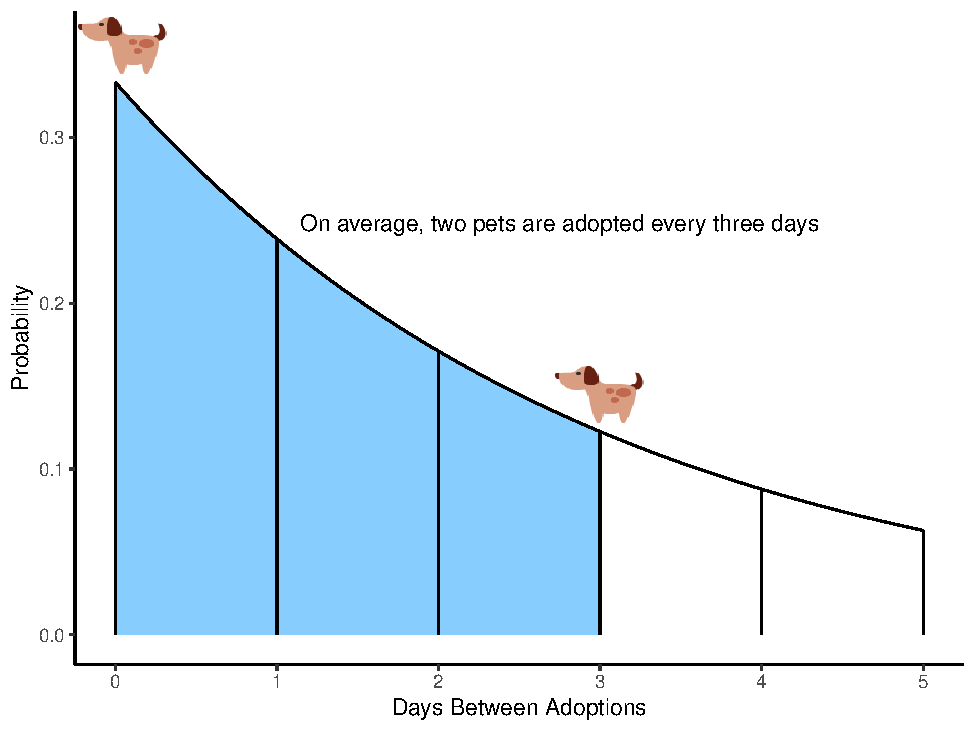
\includegraphics[width=0.6\linewidth]{famousdistrib_files/figure-latex/dogplot-1} 

}

\caption{Exponential plot with dogs}\label{fig:dogplot}
\end{figure}

\begin{center}\rule{0.5\linewidth}{0.5pt}\end{center}

\hypertarget{Gamma}{%
\subsection{Gamma Distribution}\label{Gamma}}

The exponential distribution is quite similar to the \protect\hyperlink{geometric}{geometric} distribution since they both consider the amount of time it takes for one event to occur. The main difference between the two is that geometric random variables model Bernoulli or binary processes and exponential random variables model poisson ones. Bernoulli processes consider independent trials, so if each trial is a day then we would ignore the possibility of having more than one adoption or ``success'' per day. Some might consider changing the trial unit to each animal in the shelter, but we cannot determine the probability of each animal being adopted, and we also can't assume that they each animal's probability is the same.

If \(N\) is based on poisson processes and has parameter \(\lambda\), the rate, \(N\) represents the amount of time we must wait until \(r\) events, thus following the \textbf{gamma distribution}.

\[ P(N=n)=\frac{\lambda^r}{\Gamma(r)}n^{r-1}e^{-\lambda n} \quad \textrm{for} \enspace k>0\]
If the \(\Gamma\) (Gamma) function in the equation looks new to you, you can read more about it \href{https://www.cantorsparadise.com/the-beautiful-gamma-function-and-the-genius-who-discovered-it-8778437565dc}{here}.

When \(r=1\) the equation simplifies to the exponential distribution, making it a special case similar to the geometric distribution.

\[ \begin{split}f(k)&=\frac{\lambda^1}{\Gamma(1)}k^{1-1}e^{-\lambda k} \\
&= \frac{\lambda}{1}k^0e^{-\lambda k} \\
&= \lambda e^{-\lambda k}
\end{split}\]

Returning to the adoption example, the gamma distribution lets us figure out the number of days that it takes for \textbf{more than} one adoption to occur in an interval of time.

For example, what is the probability that it takes less than 2 weeks for 3 pets to be adopted if 10 pets are adopted every month?

Recall that \(\lambda = 1/3\), assuming that an adoption is equally likely to occur every day of the month. Therefore, if \(K\) is a gamma random variable for the number of days it takes for 3 adoptions to occur, we can write the probability of \(K<14 \enspace \textrm{days}\)

\[ P(K<14) = \int_0^{14} \frac{{1/3}^3}{\Gamma(3)}k^{3-1}e^{-k/3}dk \approx 0.844\]

Or, two ways using R:

\begin{Shaded}
\begin{Highlighting}[]
\CommentTok{\# Using the gamma distribution function}
\FunctionTok{pgamma}\NormalTok{(}\DecValTok{14}\NormalTok{, }\AttributeTok{shape =} \DecValTok{3}\NormalTok{, }\AttributeTok{rate =} \DecValTok{1}\SpecialCharTok{/}\DecValTok{3}\NormalTok{)}
\end{Highlighting}
\end{Shaded}

\begin{verbatim}
## [1] 0.8443188
\end{verbatim}

\begin{Shaded}
\begin{Highlighting}[]
\CommentTok{\# Is the same as writing this definite integral}
\NormalTok{gamma\_fun }\OtherTok{\textless{}{-}} \ControlFlowTok{function}\NormalTok{(k, }\AttributeTok{lambda =} \DecValTok{1}\SpecialCharTok{/}\DecValTok{3}\NormalTok{, }\AttributeTok{r =} \DecValTok{3}\NormalTok{) (lambda}\SpecialCharTok{\^{}}\NormalTok{r)}\SpecialCharTok{/}\NormalTok{(}\FunctionTok{gamma}\NormalTok{(r)) }\SpecialCharTok{*}\NormalTok{ k}\SpecialCharTok{\^{}}\NormalTok{(r}\DecValTok{{-}1}\NormalTok{) }\SpecialCharTok{*} \FunctionTok{exp}\NormalTok{(}\SpecialCharTok{{-}}\NormalTok{lambda }\SpecialCharTok{*}\NormalTok{ k)}
\FunctionTok{integrate}\NormalTok{(gamma\_fun, }\DecValTok{0}\NormalTok{, }\DecValTok{14}\NormalTok{)}
\end{Highlighting}
\end{Shaded}

\begin{verbatim}
## 0.8443188 with absolute error < 9.4e-15
\end{verbatim}

So there is an approximate 84.4\% probability that the center has 3 adoptions in two weeks. How do you think that this probability changes as we alter \(r\) or \(\lambda\)?

\begin{Shaded}
\begin{Highlighting}[]
\CommentTok{\# Create a vector of "day" values}
\NormalTok{x }\OtherTok{\textless{}{-}} \FunctionTok{seq}\NormalTok{(}\DecValTok{0}\NormalTok{, }\DecValTok{30}\NormalTok{, }\AttributeTok{by =} \FloatTok{0.01}\NormalTok{)}

\CommentTok{\# Create a tibble with four gamma distributions, each with different r and lambda values}
\NormalTok{df }\OtherTok{\textless{}{-}} \FunctionTok{tibble}\NormalTok{(x, }
             \AttributeTok{gamma\_1 =} \FunctionTok{dgamma}\NormalTok{(x, }\DecValTok{3}\NormalTok{, }\DecValTok{1}\SpecialCharTok{/}\DecValTok{3}\NormalTok{), }
             \AttributeTok{gamma\_2 =} \FunctionTok{dgamma}\NormalTok{(x, }\DecValTok{5}\NormalTok{, }\DecValTok{1}\SpecialCharTok{/}\DecValTok{3}\NormalTok{),}
             \AttributeTok{gamma\_3 =} \FunctionTok{dgamma}\NormalTok{(x, }\DecValTok{5}\NormalTok{, }\DecValTok{2}\SpecialCharTok{/}\DecValTok{3}\NormalTok{),}
             \AttributeTok{gamma\_4 =} \FunctionTok{dgamma}\NormalTok{(x, }\DecValTok{5}\NormalTok{, }\DecValTok{1}\SpecialCharTok{/}\DecValTok{6}\NormalTok{)) }\SpecialCharTok{\%\textgreater{}\%} 
  \CommentTok{\# Transform the data frame into longer format}
  \FunctionTok{pivot\_longer}\NormalTok{(}\AttributeTok{cols =} \DecValTok{2}\SpecialCharTok{:}\DecValTok{5}\NormalTok{, }\AttributeTok{names\_to =} \StringTok{"Distribution"}\NormalTok{, }\AttributeTok{values\_to =} \StringTok{"Density"}\NormalTok{)}

\CommentTok{\# Now plot!}
\FunctionTok{ggplot}\NormalTok{(df, }\FunctionTok{aes}\NormalTok{(}\AttributeTok{x =}\NormalTok{ x, }\AttributeTok{y =}\NormalTok{ Density, }\AttributeTok{color =}\NormalTok{ Distribution)) }\SpecialCharTok{+}
  \FunctionTok{geom\_line}\NormalTok{(}\FunctionTok{aes}\NormalTok{(}\AttributeTok{group =}\NormalTok{ Distribution)) }\SpecialCharTok{+}
  \FunctionTok{labs}\NormalTok{(}\AttributeTok{x =} \StringTok{"Days"}\NormalTok{, }\AttributeTok{y =} \StringTok{"Density"}\NormalTok{) }\SpecialCharTok{+}
  \FunctionTok{scale\_color\_viridis\_d}\NormalTok{(}\AttributeTok{labels =} \FunctionTok{c}\NormalTok{(}\StringTok{"r = 3, lambda = 1/3"}\NormalTok{,}
                                \StringTok{"r = 5, lambda = 1/3"}\NormalTok{,}
                                \StringTok{"r = 5, lambda = 2/3"}\NormalTok{,}
                                \StringTok{"r = 5, lambda = 1/6"}\NormalTok{))}
\end{Highlighting}
\end{Shaded}

\begin{center}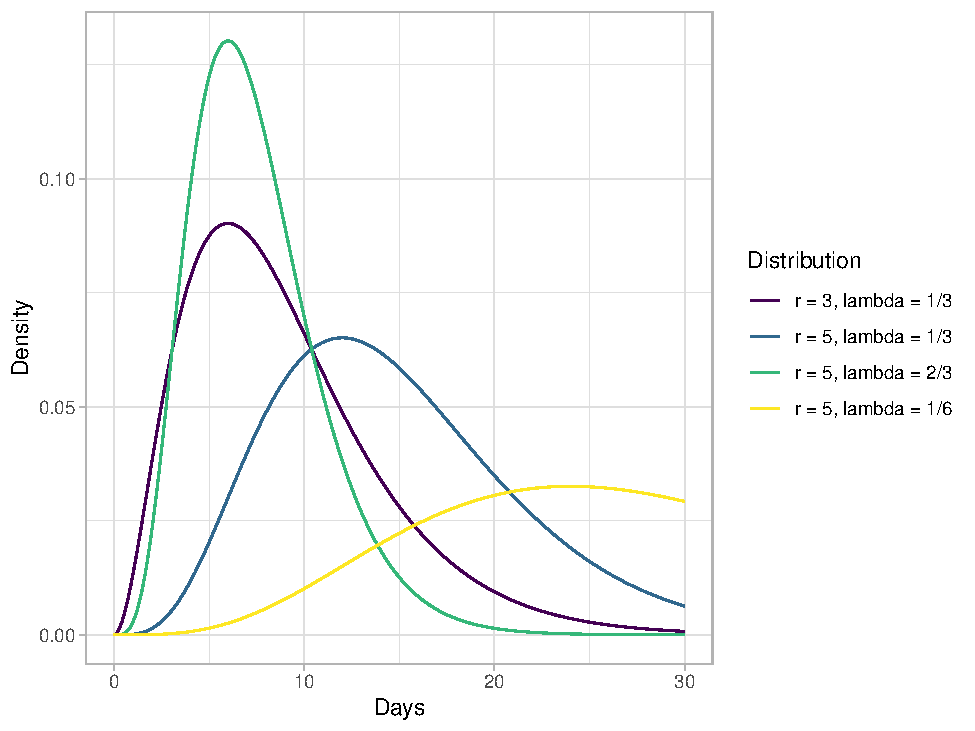
\includegraphics[width=0.6\linewidth]{famousdistrib_files/figure-latex/gamma plot-1} \end{center}

\begin{center}\rule{0.5\linewidth}{0.5pt}\end{center}

\hypertarget{ux3c72-distribution}{%
\subsection{χ2 Distribution}\label{ux3c72-distribution}}

The \(\chi^2\) distribution is extremely helpful in the statistics world, whether used for hypothesis testing as well as modeling. For instance, \textbf{\(\chi^2\) tests of independence} are used to determine whether associations between variables/categories are \emph{significant}. The test statistic that results from \textbf{\(\chi^2\) goodness of fit tests} also follow a \(\chi^2\) distribution and is equipped when researchers want to investigate whether observed data follow certain ratios. Although modeling is beyond the lens of this guide, the test statistic from \href{https://www.itl.nist.gov/div898/handbook/apr/section2/apr233.htm}{likelihood ratio tests} follow a \(\chi^2\) distribution and assess whether newer and larger models significantly improve upon older and simpler ones.

We now know the uses of the \(\chi^2\) distribution. But what actually is it? In a previous section, we learned that the \protect\hyperlink{gamma}{gamma} distribution models the probability of \(r\) events occurring in a certain period of time, given that it is based on Poisson processes. The \(\chi^2\) distribution is a specific case of the gamma distribution in which the parameters \(\lambda = 1/2\) and \(r=k/2\) where k is the degrees of freedom. After plugging in these parameters, this form of the gamma distribution can be written as:

\[f(x)=\frac{x^{k/2-1}e^{-x/2}}{2^{k/2}\Gamma(k/2)} \enspace \textrm{for} \enspace x \geq 0\]

Below is a plot of several \(\chi^2\) distributions with different degrees of freedom.

\begin{Shaded}
\begin{Highlighting}[]
\NormalTok{x }\OtherTok{\textless{}{-}} \FunctionTok{seq}\NormalTok{(}\DecValTok{0}\NormalTok{, }\DecValTok{10}\NormalTok{, }\AttributeTok{by =} \FloatTok{0.2}\NormalTok{) }\CommentTok{\# Vector of possible values}

\NormalTok{chisq\_1 }\OtherTok{\textless{}{-}} \FunctionTok{dchisq}\NormalTok{(x, }\DecValTok{1}\NormalTok{)}
\NormalTok{chisq\_2 }\OtherTok{\textless{}{-}} \FunctionTok{dchisq}\NormalTok{(x, }\DecValTok{4}\NormalTok{)}
\NormalTok{chisq\_3 }\OtherTok{\textless{}{-}} \FunctionTok{dchisq}\NormalTok{(x, }\DecValTok{8}\NormalTok{)}

\NormalTok{df }\OtherTok{\textless{}{-}} \FunctionTok{tibble}\NormalTok{(x, chisq\_1, chisq\_2, chisq\_3) }\SpecialCharTok{\%\textgreater{}\%}
  \FunctionTok{rename}\NormalTok{(}\StringTok{\textasciigrave{}}\AttributeTok{1}\StringTok{\textasciigrave{}} \OtherTok{=}\NormalTok{ chisq\_1, }\StringTok{\textasciigrave{}}\AttributeTok{4}\StringTok{\textasciigrave{}} \OtherTok{=}\NormalTok{ chisq\_2, }\StringTok{\textasciigrave{}}\AttributeTok{8}\StringTok{\textasciigrave{}} \OtherTok{=}\NormalTok{ chisq\_3) }\SpecialCharTok{\%\textgreater{}\%} 
  \FunctionTok{pivot\_longer}\NormalTok{(}\AttributeTok{cols =} \DecValTok{2}\SpecialCharTok{:}\DecValTok{4}\NormalTok{, }\AttributeTok{names\_to =} \StringTok{"Degrees of Freedom"}\NormalTok{, }\AttributeTok{values\_to =} \StringTok{"Density"}\NormalTok{)}

\FunctionTok{ggplot}\NormalTok{(df, }\FunctionTok{aes}\NormalTok{(}\AttributeTok{x =}\NormalTok{ x, }\AttributeTok{y =}\NormalTok{ Density, }\AttributeTok{color =} \StringTok{\textasciigrave{}}\AttributeTok{Degrees of Freedom}\StringTok{\textasciigrave{}}\NormalTok{)) }\SpecialCharTok{+}
  \FunctionTok{geom\_line}\NormalTok{() }\SpecialCharTok{+}
  \FunctionTok{scale\_x\_continuous}\NormalTok{(}\AttributeTok{name =} \StringTok{"Value"}\NormalTok{, }\AttributeTok{breaks =} \FunctionTok{seq}\NormalTok{(}\DecValTok{0}\NormalTok{, }\DecValTok{10}\NormalTok{, }\AttributeTok{by =} \DecValTok{2}\NormalTok{))}
\end{Highlighting}
\end{Shaded}

\begin{figure}

{\centering 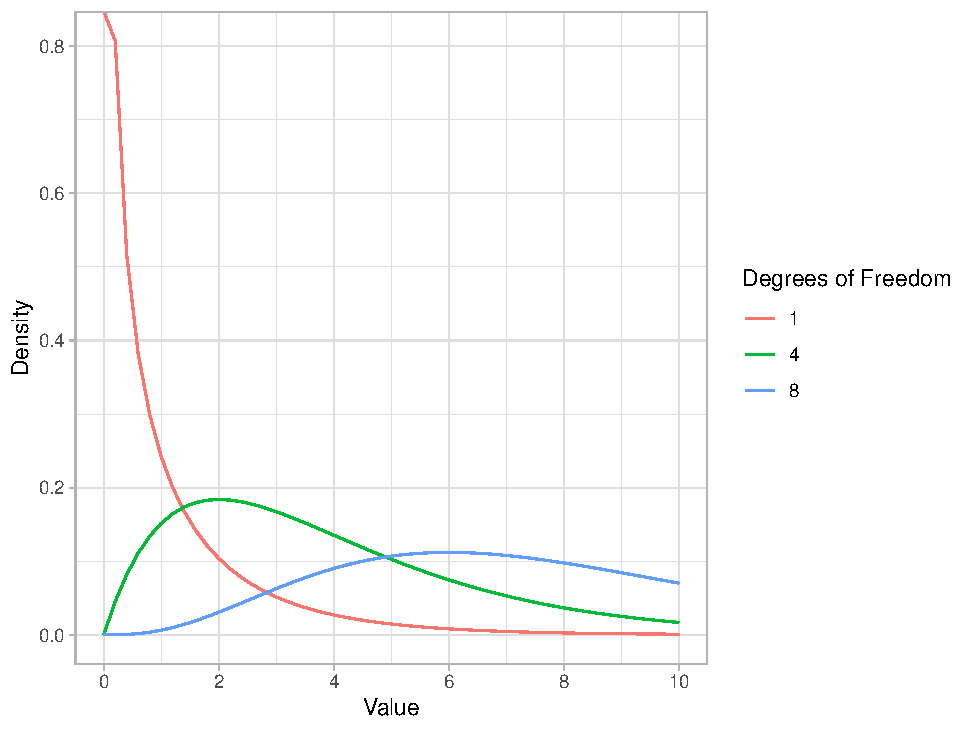
\includegraphics[width=0.6\linewidth]{famousdistrib_files/figure-latex/multChisq-1} 

}

\caption{Chi-square Distributions with 1, 4, and 8 degrees of freedom}\label{fig:multChisq}
\end{figure}

\begin{center}\rule{0.5\linewidth}{0.5pt}\end{center}

\hypertarget{chi-square-and-normal-relationship}{%
\subsubsection{Chi-square and Normal Relationship}\label{chi-square-and-normal-relationship}}

We previously learned that random deviates from the normal distribution can be taken using \texttt{rnorm}. All Chi-square distributions can be thought of as the sum of these squared and independent deviates. We can therefore also write the Chi-square distribution with k degrees of freedom as:

\[\sum_{i=1}^{k}Z_i^2 = Z_1^2 + Z^2_2 + \ldots + Z^2_k \sim \chi^2_{(k)}\]

Where each of the \(Z^2_1,Z^2_2\ldots Z^2_k\) are independent and squared random variables following the standard normal distribution.

The simplest chi-square distribution is derived from one squared and standard normal random variable (i.e.~mean = 0, standard deviation = 1). If the new random variable \(Y=Z_1^2\), then we can define Y as a chi-square random variable with \(k=1\) degrees of freedom, \(\chi^2_{(1)}\).

The plot below shows the relationship between the two random variables. It is difficult to decipher visually, but the densities for each value of the chi-square distribution are the same as normal distribution at the square root of those values. This perhaps most obvious at the intercept at \texttt{x=1} since the square root of 1 is 1. We can also draw a segment between 3 and \(\sqrt{3}\).

\begin{Shaded}
\begin{Highlighting}[]
\FunctionTok{ggplot}\NormalTok{() }\SpecialCharTok{+}
  \FunctionTok{stat\_function}\NormalTok{(}\AttributeTok{fun =}\NormalTok{ dnorm,}
                \AttributeTok{color =} \StringTok{"darkblue"}\NormalTok{) }\SpecialCharTok{+}
  \FunctionTok{stat\_function}\NormalTok{(}\AttributeTok{fun =}\NormalTok{ dchisq,}
                \AttributeTok{args =} \FunctionTok{list}\NormalTok{(}\AttributeTok{df =} \DecValTok{1}\NormalTok{),}
                \AttributeTok{color =} \StringTok{"forestgreen"}\NormalTok{) }\SpecialCharTok{+}
  \FunctionTok{annotate}\NormalTok{(}\AttributeTok{label =} \StringTok{"Normal Distribution"}\NormalTok{, }\AttributeTok{geom =} \StringTok{"label"}\NormalTok{, }\AttributeTok{x =} \FloatTok{0.5}\NormalTok{, }\AttributeTok{y =} \FloatTok{0.15}\NormalTok{, }\AttributeTok{color =} \StringTok{"darkblue"}\NormalTok{) }\SpecialCharTok{+}
  \FunctionTok{annotate}\NormalTok{(}\AttributeTok{label =} \StringTok{"Chi{-}square Distribution"}\NormalTok{, }\AttributeTok{geom =} \StringTok{"label"}\NormalTok{, }\AttributeTok{x =} \DecValTok{2}\NormalTok{, }\AttributeTok{y =} \FloatTok{0.3}\NormalTok{, }\AttributeTok{color =} \StringTok{"forestgreen"}\NormalTok{) }\SpecialCharTok{+}
  \FunctionTok{labs}\NormalTok{(}\AttributeTok{x =} \StringTok{"Value"}\NormalTok{, }\AttributeTok{y =} \StringTok{"Density"}\NormalTok{) }\SpecialCharTok{+}
  \FunctionTok{xlim}\NormalTok{(}\DecValTok{0}\NormalTok{, }\DecValTok{4}\NormalTok{) }\SpecialCharTok{+}
  \FunctionTok{ylim}\NormalTok{(}\DecValTok{0}\NormalTok{, }\FloatTok{0.5}\NormalTok{)}
\end{Highlighting}
\end{Shaded}

\begin{figure}

{\centering 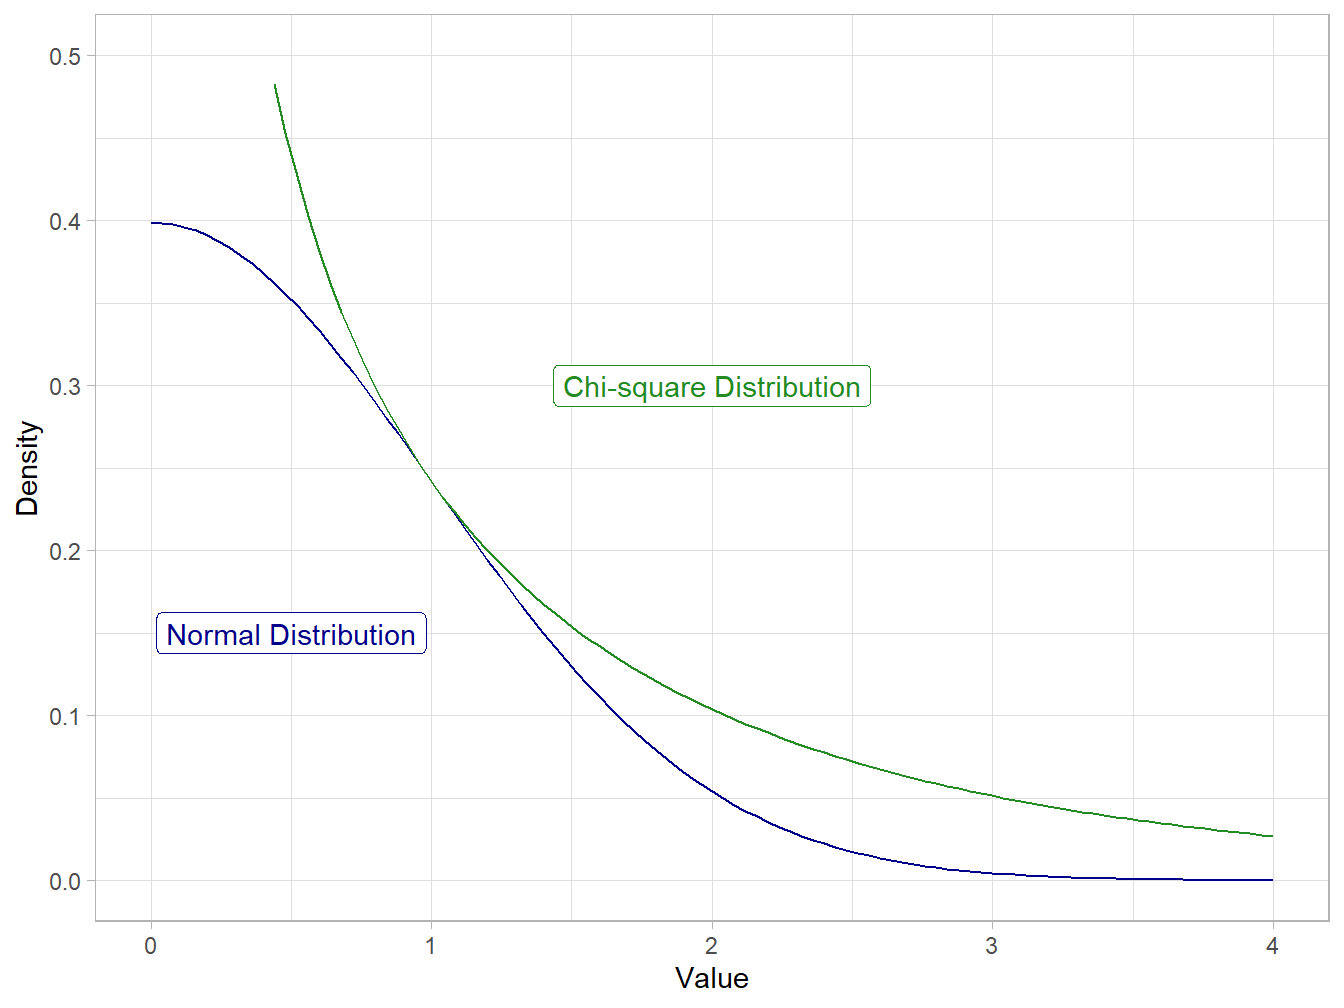
\includegraphics[width=0.6\linewidth]{famousdistrib_files/figure-latex/chisqnormal-1} 

}

\caption{Plot of the Chi-square distribution with 1 df and standard normal distribution}\label{fig:chisqnormal}
\end{figure}

We can use this specific chi-square distribution with one degree of freedom to find the cumulative densities in a normal distribution. All that we have to do is acknowledge that our chi-square random variable is a standard normal random variable squared. In other words, if \(P(Z=x)=P(Z^2=x^2)\), i.e.~the cumulative densities do not change after rewriting this chi-square distribution as the standard normal distribution squared.

For instance, the probability that a normal random variable \(Z\) is between -1.28 and 1.28 can be calculated with two methods: first by using the standard normal distribution and the second using the chi-square distribution with \(k=1\) degrees of freedom.

\[ P(-1.28 < Z <1.28) \approx 0.8 \\ P(Z^2<1.28^2) = P(|Z| < 1.28) =(\chi^2_{(1)}<1.6384) \approx 0.8\]

Similarly with R,

\begin{Shaded}
\begin{Highlighting}[]
\FunctionTok{pnorm}\NormalTok{(}\FloatTok{1.28}\NormalTok{) }\SpecialCharTok{{-}} \FunctionTok{pnorm}\NormalTok{(}\FloatTok{1.28}\NormalTok{, }\AttributeTok{lower.tail =} \ConstantTok{FALSE}\NormalTok{)}
\end{Highlighting}
\end{Shaded}

\begin{verbatim}
## [1] 0.7994549
\end{verbatim}

\begin{Shaded}
\begin{Highlighting}[]
\FunctionTok{pchisq}\NormalTok{(}\FloatTok{1.6384}\NormalTok{, }\AttributeTok{df =} \DecValTok{1}\NormalTok{)}
\end{Highlighting}
\end{Shaded}

\begin{verbatim}
## [1] 0.7994549
\end{verbatim}

Both of which can be rounded to 0.8.

We eventually use the chi-square distribution to observe more complicated situations with multiple independent and normal processes. For more the derivation of chi-square distributions with greater than 1 degrees of freedom, or if you want to learn more about this topic, see a full proof \href{https://en.wikipedia.org/wiki/Proofs_related_to_chi-squared_distribution}{here}.

\begin{center}\rule{0.5\linewidth}{0.5pt}\end{center}

\hypertarget{using-chi-square-distributions-for-testing}{%
\subsubsection{Using Chi-square Distributions for Testing}\label{using-chi-square-distributions-for-testing}}

Similar to previous distributions used for testing, we must reasonably assume that each observation in the data is independent of each other. The size condition can be confirmed by looking at whether each category in the analysis has at least \(x\) observations. In general, statisticians look to make sure that the observed counts are greater than 5, but the threshold can change depending on the circumstance.

The degrees of freedom can be calculated as \(k=(n-1)(i-1)\) where the sample as \(n\) observations and there are \(i\) categories. Similar to the t-distribution, the degrees of freedom increases as we use larger data sets with more categories or observations.

After we have determined the degrees of freedom, we calculate the \(\chi^2\) test statistic using the following:

\[ \begin{split} 
&\chi^2 =  \sum_{i=1}^{n}\frac{(O_i-E_i)^2}{E_i} \\
\textrm{Where} \enspace &O_i \enspace \textrm{is the observed count of the ith category} \\ 
&E_i \enspace \textrm{is the expected count of the ith category}
\end{split}\]

The function \texttt{chisq.test} also accomplishes this. What you provide in the function depends on whether you are doing a test for goodness of fit or independence.

For \textbf{goodness of fit} tests (whether observed data follows expected ratios), you need to create two vectors:

\begin{Shaded}
\begin{Highlighting}[]
\CommentTok{\# Create vector of probabilities}
\NormalTok{predicted }\OtherTok{\textless{}{-}} \FunctionTok{c}\NormalTok{(}\FloatTok{0.6}\NormalTok{, }\FloatTok{0.3}\NormalTok{, }\FloatTok{0.1}\NormalTok{)}

\CommentTok{\# Create vector of observed values}
\NormalTok{observed }\OtherTok{\textless{}{-}} \FunctionTok{c}\NormalTok{(}\DecValTok{66}\NormalTok{, }\DecValTok{27}\NormalTok{, }\DecValTok{15}\NormalTok{)}

\FunctionTok{chisq.test}\NormalTok{(observed, }\AttributeTok{p =}\NormalTok{ predicted)}
\end{Highlighting}
\end{Shaded}

\begin{verbatim}
## 
##  Chi-squared test for given probabilities
## 
## data:  observed
## X-squared = 2.5556, df = 2, p-value = 0.2787
\end{verbatim}

For tests of \textbf{independence} (whether associations exist between rows and columns), you need to provide a matrix:

\begin{Shaded}
\begin{Highlighting}[]
\NormalTok{ matrix }\OtherTok{\textless{}{-}} \FunctionTok{matrix}\NormalTok{(}\FunctionTok{c}\NormalTok{(}\DecValTok{103}\NormalTok{, }\DecValTok{150}\NormalTok{, }\DecValTok{103}\NormalTok{, }\DecValTok{102}\NormalTok{, }\DecValTok{140}\NormalTok{, }\DecValTok{97}\NormalTok{),}
                 \AttributeTok{nrow =} \DecValTok{2}\NormalTok{, }\AttributeTok{ncol =} \DecValTok{3}\NormalTok{, }\AttributeTok{byrow =} \ConstantTok{TRUE}\NormalTok{, }
                 \AttributeTok{dimnames =} \FunctionTok{list}\NormalTok{(}\FunctionTok{c}\NormalTok{(}\StringTok{"Group A"}\NormalTok{, }\StringTok{"Group B"}\NormalTok{), }
                                 \FunctionTok{c}\NormalTok{(}\StringTok{"Variable 1"}\NormalTok{, }\StringTok{"Variable 2"}\NormalTok{, }\StringTok{"Variable 3"}\NormalTok{)))}

\NormalTok{knitr}\SpecialCharTok{::}\FunctionTok{kable}\NormalTok{(matrix)}
\end{Highlighting}
\end{Shaded}

\begin{tabular}{l|r|r|r}
\hline
  & Variable 1 & Variable 2 & Variable 3\\
\hline
Group A & 103 & 150 & 103\\
\hline
Group B & 102 & 140 & 97\\
\hline
\end{tabular}

\begin{Shaded}
\begin{Highlighting}[]
\FunctionTok{chisq.test}\NormalTok{(matrix)}
\end{Highlighting}
\end{Shaded}

\begin{verbatim}
## 
##  Pearson's Chi-squared test
## 
## data:  matrix
## X-squared = 0.11395, df = 2, p-value = 0.9446
\end{verbatim}

Great! This concludes the last distribution in this guide. Thank you so much for reading this guide, and I wish you luck as you continue your statistics journey! :)

  \bibliography{book.bib,packages.bib}

\end{document}
